% Meta-monografia de exemplo genérico de uso da classe delaetex.cls
% Copyright (C) 2004..2016 Walter Fetter Lages <fetter@ece.ufrgs.br>
%
% This file was adapted from:
% Meta-monografia de exemplo genérico de uso da classe deletex.cls
% Copyright (C) 2004 Walter Fetter Lages <w.fetter@ieee.org>
%
% This is free software, distributed under the GNU GPL; please take
% a look in `deletex.cls' to see complete information on using, copying
% and redistributing these files
%


\documentclass[repeatfields,oneside,overleaf]{tcc}
\addbibresource{Referencias.bib}

%%%%%%%%%%%%%%%%%%%%%%
%%%%%%%%%%%%%%%%%%%%%%
%%
%% TCC Class options
%%
%% overleaf   => COMPATIBILITY workarounds for (non up to date/broke) overleaf system
%%     \documentclass[overleaf]{tcc}
%%
%% english   => paper/report in english
%%     \documentclass[english]{tcc}
%%
%% repeatfields => (abnt) references with same authors have their names repeated.
%%												otherwise only the first reference of them will be printed.
%%     \documentclass[repeatfields]{tcc}
%%
%% openright => force the start of a chapter at odd pages.
%%     \documentclass[openright]{tcc}
%%
%% oneside => single side document
%%     \documentclass[oneside]{tcc}
%%
%% NOTE : openright, oneside :: IF you are going to print the doc, single sided, the best is to just use
%%                              the [oneside] option.
%%                              IF you are going to print the doc, double sided, the best is to just use the
%%                              the [openright] option.
%%
%% relnum => figures/tables counters are reset with each chapter.
%%     \documentclass[relnum]{tcc}
%%
%% showframe => (for drafts only) auxiliary visual guide to page frame. Loads package showframe
%%     \documentclass[showframe]{tcc}
%%
%% showlabels =>  (for drafts only) prints labes/citeref strings on the side bar. Loads package showlabels
%%     \documentclass[showlabels]{tcc}
%%
%% report => for simple report generation (only first cover page, no description or approval pages).
%%     \documentclass[report]{tcc}
%%
%% internship => fields adjustment for ´internship report´
%%     \documentclass[report,internship]{tcc}
%%
%% NOTE: with the report option,
%%                       the \course{} name is optional (one can remove it with \courseundef )
%%											 the \authorinfo{}{} is mandatory
%%       without the report option,
%%                       the \course{} name is mandatory
%%											 the \authorinfo{}{} is optional for the main work,
%%																	but mandatory for the many forms
%%
%%
%%
%%%%%%%%%%%%%%%%%%%%%%
%%
%% pre-loaded packages
%%
%%
%% fontenc with T1
%%           % needed for inputenc and babel to work correctly together
%%           % https://www.ctan.org/pkg/fontenc
%% inputenc with utf8
%%           % to allow source files with utf8 encoding.
%%           % https://www.ctan.org/pkg/inputenc
%% babel
%%           % better word typography (line breaking and all...), language dependent
%%           % https://www.ctan.org/pkg/babel
%%           % https://www.ctan.org/pkg/babel-portuges
%% csquotes
%%           % better quotation system
%%           % https://www.ctan.org/pkg/csquotes
%% biblatex with biber backend and abnt style
%%           % for bibliography
%%           % https://www.ctan.org/pkg/biblatex
%%           % https://www.ctan.org/pkg/biber
%%           % https://www.ctan.org/pkg/biblatex-abnt
%% silence
%%           % to remove (silence) some silly biblatex (abnt) warnings.
%%           % https://www.ctan.org/pkg/silence
%% lastpage
%%           % enables, e.g. footprint, a reference to the last page.
%%           % https://www.ctan.org/pkg/lastpage
%% url
%%           % correct display of URLs
%%           % https://www.ctan.org/pkg/url
%% enumerate
%%           % to use characters instead of numbers in enumerate/list environments
%%           % https://www.ctan.org/pkg/enumerate
%% keyval
%%           % process ´key=val´ as a macro parameter. needed by graphicx
%%           % https://www.ctan.org/pkg/keyval
%% graphicx
%%           % pic insertion
%%           % https://www.ctan.org/pkg/graphicx
%% mathptmx
%%           % use of Times New Roman including math environment
%%           % https://www.ctan.org/pkg/mathptmx
%% amsmath, amsthm, amssymb, mathrsfs, amsfonts
%%           % diversas fontes para modo math
%%           % http://www.ams.org/publications/authors/tex/amslatex
%%           % http://mirror.ctan.org/info/short-math-guide
%%           % https://www.ctan.org/pkg/amsmath
%%           % https://www.ctan.org/pkg/amsthm
%%           % https://www.ctan.org/pkg/amssymb
%%           % https://www.ctan.org/pkg/mathrsfs
%%           % https://www.ctan.org/pkg/amsfonts
%% mathtools
%%           % extension and bug fixes to amsmath
%%           % https://www.ctan.org/pkg/mathtools
%% empheq, cases, extarrows
%%           % extension  to amsmath
%%           % https://www.ctan.org/pkg/empheq
%%           % https://www.ctan.org/pkg/cases
%%           % https://www.ctan.org/pkg/extarrows
%% mathfixs
%%           % some adjustments (spacing)
%%           % https://www.ctan.org/pkg/mathfixs
%% fp
%%           % support for simple fixed point math
%%           % https://www.ctan.org/pkg/fp
%% multirow
%%           % allow the definition of a multirow cell in a tab environment
%%           % https://www.ctan.org/pkg/multirow
%% bigdelim
%%           % allow the use of big delimiters in tabular/array
%%           % https://www.ctan.org/pkg/bigdelim
%% longtable
%%           % allow the creation of a multi page table.
%%           % https://www.ctan.org/pkg/longtable
%% listings
%%           % add an environment for ´source code´ (verbatin) with sintax highlight.
%%           % https://www.ctan.org/pkg/listings
%% xcolor
%%           % custom color definions. used by listings.
%%           % https://www.ctan.org/pkg/xcolor
%% newfloat
%%           % (re)definition of custom float environments, and associated ´table of...´
%%           % https://www.ctan.org/pkg/newfloat
%% caption
%%           % fine adjustments and better caption handling.
%%           % https://www.ctan.org/pkg/caption
%% circuitikz
%%           % graphics and circuits drawing environment (includes pgf/tikz).
%%           % https://www.ctan.org/pkg/circuitikz
%%           % https://www.ctan.org/pkg/pgf
%% steinmetz
%%           % writing complex numbers in polar form (\phase).
%%           % https://www.ctan.org/pkg/steinmetz
%%
%%%%%%%%%%%%%%%%%%%%%%
%%%%%%%%%%%%%%%%%%%%%%

\usepackage{subcaption}
\usepackage{placeins}
\usepackage{indentfirst}
%\usepackage[hidelinks]{hyperref}
\usepackage[
    pdfauthor={Guilherme de Paoli Beal},
    pdftitle={Projeto de Controlador PMR Sintonizado por VRFT para Rejeicao de Harmonicas em Fonte de Alimentacao Ininterrupta},
    hidelinks
]
    {hyperref}
\usepackage{siunitx}
\usepackage{textgreek}
\usepackage{icomma}


% \usepackage[pdftex,
%             pdfauthor={Your Name},
%             pdftitle={The Title},
%             pdfsubject={The Subject},
%             pdfkeywords={Some Keywords},
%             pdfproducer={Latex with hyperref, or other system},
%             pdfcreator={pdflatex, or other tool}]{hyperref}

\newcommand{\matr}[1]{\mathbf{#1}}

%%%%%%%%%%%%%%%%%%%%%%
%%%%%%%%%%%%%%%%%%%%%%
%
% Meus comandos personalizados para minhas variáveis
%

\newcommand{\mycdot}{ \, }

\newcommand{\myvo}{ {v_o} }
\newcommand{\myilf}{ {i{_{L_f}}} }

\newcommand{\myC}[2][]{ C_{#1} \left( #2 \right) }
\newcommand{\myG}[2][]{ G_{#1} \left( #2 \right) }
\newcommand{\myT}[2][]{ T_{#1} \left( #2 \right) }

\newcommand{\myoC}[2][]{ \overline{C_{#1}} \left( #2 \right) }
\newcommand{\myCzrho}[1]{ \myC[#1]{z, \rho_{#1}} }

\newcommand{\myCG}[3][]{ \myC[#1]{#2} \mycdot \myG[#1]{#3} }

%%%%%%%%%%%%%%%%%%%%%%
%%%%%%%%%%%%%%%%%%%%%%
%
% Minhas configurações personalizadas do tikz
%

\usetikzlibrary{positioning,calc}

\tikzstyle{block} = [draw, fill=white, rectangle, minimum height=2em, minimum width=5em]
\tikzstyle{input} = [coordinate]
\tikzstyle{output} = [coordinate]
\tikzstyle{pinstyle} = [pin edge={to-,thin,black}]

\tikzset{add/.style n args={4}{
    minimum width=2em,
    path picture={
        \draw[black]
            (path picture bounding box.south east) -- (path picture bounding box.north west)
            (path picture bounding box.south west) -- (path picture bounding box.north east);
        \node at ($(path picture bounding box.south)+(0,0.175)$)     {\footnotesize #1};
        \node at ($(path picture bounding box.west)+(0.175,0)$)      {\footnotesize #2};
        \node at ($(path picture bounding box.north)+(0,-0.175)$)    {\footnotesize #3};
        \node at ($(path picture bounding box.east)+(-0.175,0)$)     {\footnotesize #4};
        }
    }
}

%%% Separação silábica

\hyphenation{MATLAB, Simulink, PSIM, Simulink/MATLAB, ISO/IEC, 62040-3:2011}

%%%%%%%%%%%%%%%%%%%%%%
%%%%%%%%%%%%%%%%%%%%%%
%
% inicio do documento
%
\begin{document}

% O comando \maketile gera a capa, a folha de rosto e a folha de aprovacao
% (se for o caso)
\maketitle


% dedicatoria é opcional
\chapter*{Dedicatória}

À minha vó Delmina --- a Delma --- e seu ânimo inspirador.

% agradecimentos são opcionais
\chapter*{Agradecimentos}

Eu tenho muito a agradecer...
\\\\

Ao pai Ademir e à mãe Silvana, pela confiança e pela provisão de todos os recursos. Obrigado!

%À tia Rita e ao tio Deca, que fazem desta Porto Alegre também um porto seguro. Obrigado!
À tia Rita e ao tio Deca, por oferecem um porto seguro dentro de Porto Alegre. Obrigado!

%À irmã Giovana, pela compreensão diária. Obrigado!

Aos amigos Fábio, Milena e William, pela prazerosa e reconfortante companhia para estudos e descontrações. Obrigado!

Aos gêmeos, Vinícius e Leonardo, por estarem há tantos anos me acompanhando. Obrigado!

À querida Camila, pelas tantas emoções compartilhadas. Obrigado!

A tantos outros amigos, de perto e de longe, pela presença em bons e maus momentos. Obrigado!

Aos altruístas companheiros do Centro dos Estudantes de Engenharia de Controle e Automação (CEECA), por embarcarem em algumas das minhas ideias. Obrigado!

À amada e odiada Universidade Federal do Rio Grande do Sul (UFRGS), pelas tantas oportunidades. Obrigado!

A todos os professores, da pré-escola à graduação, por expandirem meus horizontes. Obrigado!

À orientadora Lucíola, por idealizar e supervisionar este trabalho. Obrigado!

Ao coorientador Charles, pelas sugestões no desenvolvimento e minuciosa revisão. Obrigado!

Aos profissionais de saúde e outros serviços essenciais, por protegerem nossas vidas em meio a uma pandemia. Obrigado!
\\\\

Sem vocês eu não haveria realizado o que realizei. Muito obrigado!

% resumo no idioma do documento
\begin{abstract}

\noindent
Este trabalho aplica uma topologia de controle em cascata para acionar o estágio de saída de uma fonte de alimentação ininterrupta.
No laço externo, um controlador proporcional-múltiplo-ressonante atua sobre o erro de seguimento de referência.
Internamente, a corrente no indutor do filtro de saída é realimentada por um controlador proporcional.
Essa configuração possibilita o seguimento de uma referência senoidal de frequência pré-estabelecida, bem como a rejeição de perturbações em suas componentes harmônicas.
A sintonia de ambos os controladores é realizada pelo método \textit{virtual reference feedback tuning}, a partir de dados coletados de um único ensaio em malha aberta, sem que seja determinado um modelo para o processo.
A dinâmica da fonte de alimentação ininterrupta é simulada pelo \textit{software} PSIM, enquanto o sistema de controle é implementado através do Simulink\slash{}MATLAB.
O desempenho do sistema em malha fechada é avaliado com base na norma ISO\slash{}IEC 62040-3:2011.
Os resultados mostram que, até a 7{\textordfeminine} harmônica, os controladores efetivamente atuam na atenuação das distorções harmônicas nas frequências para as quais são projetados, além de fornecer seguimento à referência senoidal especificada.
Para harmônicas de maior ordem, o sistema em malha fechada mostra-se instável nas condições examinadas.

\end{abstract}

% resumo no outro idioma
% como parametro devem ser passadas as palavras-chave
% no outro idioma, separadas por vírgulas
\begin{englishabstract}{Cascade Control, Data-Driven Control, Harmonic Compensation, Proportional Multi-Resonant Controller, Uninterruptible Power Supply, Virtual Reference Feedback Tuning}

\noindent
This project applies cascade control to drive the output stage of an uninterruptible power supply.
On the external loop, a proportional multi-resonant controller feedbacks the reference error.
Internally, a proportional controller takes the current through the output filter inductor.
This topology is capable of following a sinusoidal reference of pre-established frequency, as well as attenuating harmonic disturbances.
Both controllers are tuned by virtual reference feedback tuning, using data from a single open-loop experiment.
No process model is required.
The dynamics of the uninterruptible power supply are simulated using PSIM, whilst the control system is implemented through Simulink\slash{}MATLAB.
The closed-loop performance is evaluated in conformance to the ISO\slash{}IEC 62040-3:2011 standard.
Results show that, up to the 7th harmonic, the controllers effectively attenuate harmonic distortions in the frequencies for which they were designed, besides providing tracking of the specified sinusoidal reference.
For higher order harmonics, the closed-loop system becomes unstable under the tested conditions.

\end{englishabstract}

% Conforme a NBR 6027, secao 4, o sumário deve ser o último elemento pré-textual. O
% modelo do PPGEE nao atende a esta exigencia. Obviamente, a norma deveria ter a
% precedência. No entanto, neste arquivo optou-se por reproduzir o que está
% no modelo para word.



% lista de ilustrações
\listoffigures

% lista de tabelas
\listoftables

% lista de listagens (código fonte)
%\listoflistings %% doesn't work on overleaf

% lista de abreviaturas e siglas
% o parametro deve ser a abreviatura mais longa
\begin{listofabbrv}{LASCAR}
    \item[AC] \textit{Alternating Current} (Corrente Alternada)
    \item[ANEEL] Agência Nacional de Energia Elétrica
    \item[ARX] \textit{Autoregressive with Extra Input} (Autorregressiva com Entrada Externa)
    \item[BIBO] \textit{Bounded-Input, Bounded-Output} (Entrada Limitada, Saída Limitada)
    \item[DC] \textit{Direct Current} (Corrente Contínua)
    \item[IEC] \textit{International Electrotechnical Commission} (Comissão Eletrotécnica Internacional)
    \item[IGBT] \textit{Insulated Gate Bipolar Transistor} (Transistor Bipolar de Porta Isolada) % Só 1x
    \item[IHD] \textit{Individual Harmonic Distortion} (Distorção Harmônica Individual)
    \item[ISO] \textit{International Organization for Standardization} (Organização Internacional para Padronização)
    \item[LASCAR] Laboratório de Sistemas de Controle, Automação e Robótica
    \item[LC] Indutivo-Capacitivo
    %\item[LTI] \textit{Linear Time-Invariant} (Linear e Invariante no Tempo) % Só 1x
    \item[P] Proporcional
    \item[PID] Proporcional-Integral-Derivativo % Só 1x
    \item[PMI] Princípio do Modelo Interno
    \item[PMR] Proporcional-Múltiplo-Ressonante
    \item[PR] Proporcional-Ressonante
    \item[PRBS] \textit{Pseudorandom Binary Sequence} (Sequência Binária Pseudoaleatória)
    \item[PWM] \textit{Pulse Width Modulation} (Modulação por Largura de Pulso)
    \item[RC] Resistivo-Capacitivo
    \item[RMS] \textit{Root Mean Square} (Raiz do Valor Quadrático Médio)
    \item[SISO] \textit{Single-Input, Single-Output} (Única Entrada e Única Saída)
    \item[THD] \textit{Total Harmonic Distortion} (Distorção Harmônica Total)
	\item[UFRGS] Universidade Federal do Rio Grande do Sul
    \item[UPS] \textit{Uninterruptible Power Supply} (Fonte de Alimentação Ininterrupta)
    \item[VRFT] \textit{Virtual Reference Feedback Tuning} (Sintonia pela Referência Virtual Realimentada)
\end{listofabbrv}

% lista de símbolos é opcional
\begin{listofsymbols}{$ \cos(\cdot) $}

%%%% Agrupados por categoria

%% Matemática

    \item[$ \mathbb{N} $] Conjunto dos números naturais
    \item[$ \mathbb{R} $] Conjunto dos números reais
    \item[$ \mathbb{C} $] Conjunto dos números complexos

    \item[$ \in $] Pertence

    \item[$ \infty $] Infinito
    \item[$ j $] Unidade imaginária

    \item[$ \sum $] Somatório
    \item[$ \prod $] Produtório

    \item[$ \sin(\cdot) $] Função seno
    \item[$ \cos(\cdot) $] Função cosseno

    \item[$ \left| \cdot \right| $] Módulo de um número
    \item[$ \phase{\cdot} $] Argumento de um número complexo

    \item[$ \left\lVert \cdot \right\rVert_2 $] Norma euclidiana

    \item[$ \begin{bmatrix} \cdot \end{bmatrix}^T $] Matriz transposta

%% Sistemas e Sinais

    \item[$ t $] Variável de tempo contínuo
    \item[$ x(t) $] Sinal $x$ de tempo contínuo

    \item[$ k $] Variável de tempo discreto
    \item[$ x {[k]} $] Sinal $x$ de tempo discreto
    \item[$ T_s $] Período de amostragem

    \item[$ f $] Frequência no tempo contínuo
    \item[$ \omega $] Frequência angular no tempo contínuo
    \item[$ \Omega $] Frequência no tempo discreto


    \item[$ z $] Variável complexa
    \item[$ H(z) $] Função de transferência discreta de um sistema $H$
    \item[$ h {[k]} $] Resposta ao impulso de um sistema $H$

    \item[$ N_H(z) $] Numerador da função de transferência $H(z)$
    \item[$ D_H(z) $] Denominador da função de transferência $H(z)$

    \item[$ n_z $] Número de zeros de uma função de transferência
    \item[$ n_p $] Número de polos de uma função de transferência

    \item[$ z_i $] Zero de índice $i$ de uma função de transferência
    \item[$ p_i $] Polo de índice $i$ de uma função de transferência

    \item[$ \phi_u(z) $] Polinômio contendo apenas modos instáveis e marginalmente estáveis
    \item[$ \phi_s(z) $] Polinômio contendo apenas modos estáveis

%% Sistemas de Controle

    \item[$ r $] Sinal de referência
    \item[$ u $] Sinal de controle\slash{}atuação
    \item[$ y $] Sinal de saída
    \item[$ e $] Sinal de erro
    \item[$ q $] Sinal de perturbação na saída

    \item[$ C(z) $] Função de transferência do controlador
    \item[$ G(z) $] Função de transferência do processo
    \item[$ T(z) $] Função de transferência do sistema em malha fechada
    \item[$ S(z) $] Função de transferência da sensibilidade em malha fechada

    \item[$ T_d(z) $] Função de transferência desejada para o sistema em malha fechada

    \item[$ \overline{x} $] Sinal $x$ virtual

    \item[$ \rho $] Vetor linha de parâmetros do controlador parametrizado
    \item[$ \myoC{z} $] Vetor coluna de funções de transferência do controlador parametrizado

    \item[$ J_{mr} $] Custo do modelo de deferência
    \item[$ W(z) $] Filtro ponderador do custo do modelo de deferência

    \item[$ J_{vr} $] Custo de referência virtual
    \item[$ L(z) $] Filtro ponderador do custo de referência virtual

    \item[$ S_i(z) $] Função de transferência da sensibilidade interna

    \item[$ \varphi(z) $] Vetor de regressão

%% Elétricos

    \item[$ V_{DC} $] Tensão elétrica no barramento DC

    \item[$ C_i $] Capacitância genérica $i$
    \item[$ S_i $] Transistor genérico $i$

    \item[$ C_f $] Capacitância do filtro de saída
    \item[$ L_f $] Indutância do filtro de saída
    \item[$ R_{L_f} $] Resistência interna do indutor do filtro de saída

    \item[$ i_{L_f} $] Corrente elétrica no indutor do filtro de saída
    \item[$ v_o $] Tensão elétrica na saída

    \item[$ Y_o $] Admitância da carga

    \item[$ v_{tri} $] Tensão elétrica triangular para modulação

    \item[$ R_{li} $] Resistência da carga linear $i$

    \item[$ R_{si} $] Resistência de entrada da carga não linear $i$
    \item[$ R_{nli} $] Resistência do filtro RC da carga não linear $i$
    \item[$ C_{nli} $] Capacitância do filtro RC da carga não linear $i$

%% Outros

    \item[IHD\textsubscript{$i$}] IHD sobre a harmônica de ordem $i$

\end{listofsymbols}

% sumario
\setcounter{tocdepth}{3}
\tableofcontents

% AQUI COMEÇA O TEXTO PROPRIAMENTE DITO

\chapter{Introdução}\label{sec:introducao}

Os sistemas de transmissão e distribuição de energia elétrica consolidaram-se, desde o final do século XIX, a operar em corrente alternada --- em inglês, \textit{Alternating Current} (AC) --- \cite{Sadiku2013}.
Nesse modo, os sinais de tensão são caracterizados por ondas senoidais, descritas pelo valor eficaz e frequência nominais.
Além desses valores, a qualidade da energia pode ser avaliada em termos da presença de distorções harmônicas, quedas e picos de tensão, comportamento transiente, entre outros aspectos \cite{Rashid2011}.
% Perturbações na alimentação podem ocorrer, por exemplo, pela baixa capacidade do sistema de distribuição ou conexão de novos equipamentos na rede.

No Brasil, a Agência Nacional de Energia Elétrica (ANEEL) é responsável pela regulação do setor elétrico.
Em todo o país, a frequência nominal da rede é de $60 \text{ Hz}$.
Na distribuição, a tensão eficaz nominal varia de acordo com o tipo de instalação e local.
%Para instalações domésticas, predominam as instalações monofásicas de $127 \text{ V}$ ou $220 \text{ V}$, ou bifásicas de $220 \text{ V} / 127 \text{ V}$.
Nos Procedimentos de Distribuição de Energia Elétrica no Sistema Elétrico Nacional \cite{PRODIST} são estabelecidos os critérios para avaliação da qualidade da energia elétrica.
%Por exemplo, em instalações domésticas de baixa tensão, sob operação normal, são aceitáveis variações de tensão eficaz em até $5\%$ do seu valor nominal, enquanto a frequência pode flutuar em $0,1 \text{ Hz}$.
Por exemplo, em instalações domésticas de baixa tensão são aceitáveis variações de tensão eficaz em até $5\%$ do seu valor nominal, enquanto a frequência pode flutuar em $0,1 \text{ Hz}$.

Ocorre que certos equipamentos podem ser sensíveis a essas e outras variações na alimentação.
Neste contexto, a fonte de alimentação ininterrupta --- \textit{Uninterruptible Power Supply} (UPS) --- é um sistema de potência capaz de fornecer alimentação elétrica ininterrupta, confiável e de alta qualidade, conectado entre a rede e os equipamentos.
Além de eliminar perturbações provindas da rede, a UPS é também capaz de substituí-la temporariamente em caso de interrupção do fornecimento.
%Outra vantagem proporcionada por UPSs é o isolamento elétrico entre a carga e a rede.
Aplicações típicas incluem instalações hospitalares, armazenamento de dados, equipamentos de emergência e sistemas de telecomunicação \cite{Rashid2011}.

Em uma UPS monofásica \textit{online}, o estágio de saída é composto por um inversor em meia ponte e um filtro indutivo-capacitivo (LC).
O objetivo deste sistema é alimentar uma carga com uma tensão senoidal de amplitude e frequências constantes.
Para tanto, o inversor deve realizar a conversão de energia armazenada em corrente contínua --- \textit{Direct Current} (DC) --- para AC.

O inversor é acionado por modulação por largura de pulso --- \textit{Pulse Width Modulation} (PWM).
Um sistema de controle é aplicado para proporcionar o acionamento adequado a cada instante.
Este sistema deve, através do monitoramento da tensão fornecida à carga e comparação com um sinal de referência, atuar sobre o inversor a fim de minimizar o erro entre esses sinais.
Deve, ainda, responder adequadamente a perturbações impostas por não linearidades da carga ou por sua variação ao longo do tempo.
O desempenho do sistema de controle está diretamente relacionado ao desempenho da UPS como um todo, cujos critérios de avaliação são especificados pela norma \textcite{IEC62040-3:2011}.

Diversos trabalhos já trataram o problema do controle de UPSs, utilizando diferentes topologias e classes de controlador.
Citam-se a seguir algumas dessas contribuições.
%
\textcite{Finn1993} discute os benefícios da aplicação de um laço de controle interno, utilizando um sinal de corrente, juntamente ao laço externo para seguimento de referências senoidais em inversores.
\textcite{Abdel1996} propõem a utilização da corrente no capacitor do filtro LC para o laço interno no controle de UPSs.
\textcite{Ryan1997} apresentam topologias que aplicam a corrente no capacitor ou no indutor do filtro.
Através desses trabalhos, verifica-se que o laço interno contribui para um melhor desempenho transitório.

\textcite{Willmann2007} utilizam o controlador Proporcional-Integral-Derivativo (PID) clássico no laço externo, atuando sobre o valor eficaz da tensão de saída.
O sinal fornecido por este controlador é multiplicado pela própria referência senoidal, e somam-se a ele dois controladores Proporcionais (P), um empregando a tensão de saída e o outro a corrente no indutor.

\textcite{Loh2003} estudam os efeitos da realimentação de corrente e sugerem utilizar um controlador Proporcional-Ressonante (PR), ajustado para a frequência de referência, no controle da tensão.
\textcite{Teodorescu2006} reforçam a proposta por controladores PRs.
A fim de rejeitar perturbações harmônicas geradas por cargas não lineares, \textcite{Pereira2014, Keiel2017, Keiel2019, Bertoldi2019, Lorenzini2019} implementam um controlador Proporcional-Múltiplo-Ressonante (PMR), focando nos múltiplos ímpares da frequência fundamental.
Com esse mesmo objetivo, \textcite{Escobar2007} aplicam um controlador repetitivo.
Outros trabalhos avaliam a utilização de ambas as classes de controlador em separado \cite{Flores2012} ou em conjunto \cite{Lorenzini2013, Lorenzini2015}.
Destaca-se que, entre todos esses, \textcite{Keiel2017, Keiel2019} são os únicos a considerar o projeto discreto direto.

Técnicas não lineares de controle foram também implementadas, incluindo modos deslizantes \cite{Utkin1993, Jung1996} e \textit{deadbeat} \cite{Park2003}.
Há ainda trabalhos que realizam comparações entre diferentes estratégias \cite{Timbus2009}.

Na maioria dos trabalhos supracitados a sintonia dos controladores é realizada a partir de modelos analíticos para a UPS, como funções de transferência ou representações no espaço de estados.
Existem, porém, técnicas de controle baseadas em dados que dispensam essa etapa do projeto.
A sintonia pela referência virtual realimentada --- \textit{Virtual Reference Feedback Tuning} (VRFT) --- é um método em que o controlador é obtido a partir de dados coletados em um único ensaio sobre o sistema a ser controlado \cite{Campi2000}.

Neste contexto, \textcite{Schildt2014} emprega uma estrutura com um controlador P na malha interna, utilizando a corrente do indutor e sintonizado empiricamente, e PR na malha de tensão, sintonizado por VRFT.
\textcite{Corleta2015, Corleta2016} utilizam a mesma estrutura de controle, desta vez sintonizando ambos os controladores por VRFT, sendo um primeiro ensaio para sintonia do controlador de corrente e um segundo experimento para o controlador de tensão.
%
\textcite{Chrystian2020} apresentam um método para sintonizar os dois controladores em uma estrutura em cascata genérica a partir de dados obtidos em um único ensaio.
Tal metodologia é aplicada para desenvolver controladores para UPS, sendo PR na malha de tensão e P na de corrente, por \textcite{Bruna2020}.

O presente trabalho estuda o controle do estágio de saída de uma UPS \textit{online}.
Aplica-se um controlador PMR na malha de tensão e um controlador P na malha de corrente.
O controlador PMR é projetado para atuar nas frequências harmônicas ímpares da fundamental.
Através dessa configuração, procura-se reduzir as perturbações impostas ao sistema por cargas não lineares, avaliadas pelas distorções harmônicas total e individuais na tensão de saída.
O projeto é realizado considerando o tempo discreto.

\newpage
%Essa mesma estrutura é utilizada por \textcite{Pereira2014. Bertoldi2019}, porém ali a sintonia é realizada a partir de um modelo dinâmico da UPS.
%Neste trabalho, ambos os controladores são sintonizados pelo método VRFT a partir de um único ensaio realizado sobre o sistema.
Ambos os controladores são simultaneamente sintonizados através do método VRFT, utilizando dados de um único ensaio realizado sobre a UPS.
A modelagem deste sistema é, portanto, dispensada.
A formulação de um modelo de referência adequado mostra-se essencial nesta proposta, sendo a principal contribuição deste trabalho.

O comportamento dinâmico da UPS é simulado pelo \textit{software} PSIM.
O controlador é projetado através do \textit{software} MATLAB, e implementado por sua extensão Simulink.
%Uma simulação conjunta permite a implementação do sistema em malha fechada.
A cossimulação de ambas as partes permite a implementação do sistema em malha fechada.


% [...]

% \cite{Teodorescu2006} faz uma analogia entre o controladores PI e PR:
% o controlador PI introduz um ganho infinito para frequência nula e, portanto, proporciona seguimento ou rejeição de sinais constantes;
% já o controlador PR ideal introduz um ganho infinito em uma determinada frequência selecionada e, portanto,  proporciona seguimento ou rejeição de sinais senoidais nessa frequência.
% \cite{Teodorescu2006} também demonstra a implementação de um controlador PR para uma UPS monofásica.

% A utilização de controlador PMR é indicada por \cite{Flores2012, Pereira2014}.

% %Outras estratégias incluem o controlador repetitivo \cite{Inoue1981}.

% [...]

\chapter{Revisão da Literatura}\label{sec:revisao}

Este capítulo reúne conceitos importantes para o desenvolvimento deste trabalho.
Inicialmente é introduzida a teoria de sistemas de controle, seguido da exposição dos princípios utilizados no projeto.
Após, apresenta-se uma fonte de alimentação ininterrupta, seus componentes de interesse, e os principais critérios de desempenho.

\section{Sistemas de Controle}\label{sec:controle}

Um sistema de controle objetiva regular o comportamento de variáveis de saída de um processo através da atuação em variáveis de entrada.
O controle em malha fechada é uma estratégia clássica, em que os sinais de saída são medidos e comparados a sinais de referência, procedimento este denominado realimentação.
A partir do erro resultante, o controlador determina sinais de controle que, através de atuadores, influenciam o processo visando a aproximar o sinal de saída da referência.
Esse procedimento, considerando um processo com uma única entrada e uma única saída --- \textit{Single Input, Single Output} (SISO) ---, é ilustrado pela Figura \ref{fig:control}.

\begin{figure}[h]
    \centering
    \caption{Diagrama de um sistema de controle SISO em malha fechada.}
    \resizebox{\textwidth}{!}{%
    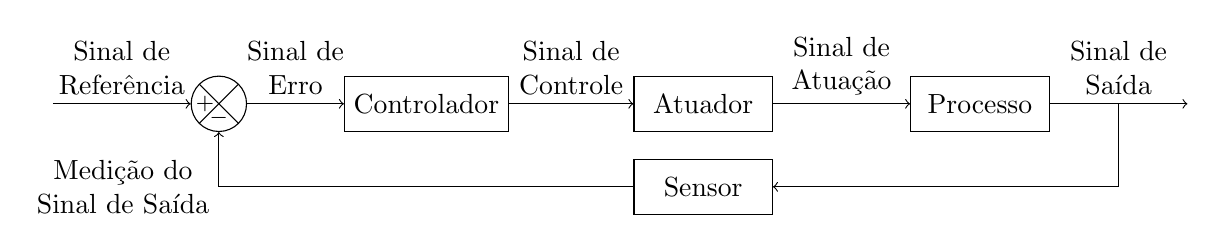
\begin{tikzpicture}[auto, node distance=7.5em]
        \node [input, name=input] {};
        \node [draw, circle, add={$-$}{$+$}{}{}, right of=input, node distance=6em] (sum) {};
        \node [block, right of=sum] (c) {Controlador};
        \node [block, right of=c, node distance=10em] (a) {Atuador};
        \node [block, right of=a, node distance=10em] (p) {Processo};
        \node [output, right of=p] (output) {};
        \node [block, below of=a, node distance=3em] (s) {Sensor};

        \draw [->, align=center] (input) -- node {Sinal de\\Referência} (sum);
        \draw [->, align=center] (sum) -- node {Sinal de\\Erro} (c);
        \draw [->, align=center] (c) -- node {Sinal de\\Controle} (a);
        \draw [->, align=center] (a) -- node {Sinal de\\Atuação} (p);
        \draw [->, align=center] (p) -- node [name=y] {Sinal de\\Saída} (output);

        \draw [->, align=center] (y) |- (s);
        \draw [->, align=center] (s) -| node {Medição do\\Sinal de Saída} (sum);
    \end{tikzpicture}
    }%
    \\\sourcecitation{adaptado de \cite{Bazanella2005}}
    \label{fig:control}
\end{figure}

Cada um dos elementos do sistema de controle pode ser considerado um sistema individual.
A dinâmica de cada um desses sistemas pode ser modelada por uma função de transferência.

Neste trabalho, serão considerados sistemas e sinais de tempo discreto.
Detalhes sobre essas representações, bem como considerações sobre a amostragem e a transformada $z$, podem ser vistos em \cite{Haykin2001, Astrom2011, Dorf2011}.
%
A discretização de um sinal de tempo contínuo $x(t)$ com um período de amostragem constante $T_s$ resulta no sinal
\begin{equation}\label{eq:sampling}
    x[k] = x(k \mycdot T_s)
    \,,\;
    \left\{ k \in \mathbb{N} \right\}
    \,.
\end{equation}
A função de transferência $H(z)$ de um sistema é definida como a transformada $z$ de sua resposta ao impulso $h[k]$, ou ainda como a razão entre as transformadas $z$ de sinais de saída e entrada correspondentes, $x_{out}(z)$ e $x_{in}(z)$:
\begin{equation}\label{eq:transfer_function}
    H(z) = \sum_{k = 0}^{\infty} h[k] \mycdot z^{-k}
         = \dfrac{ x_{out}(z) }{ x_{in}(z) }
    \,.
\end{equation}

O sistema de controle SISO em malha fechada é modelado conforme a Figura \ref{fig:feedbackloop}.
A função de transferência $\myC{z}$ representa o controlador, enquanto a função de transferência $\myG{z}$ corresponde ao conjunto do atuador com o processo.
%Sendo a dinâmica do sensor desprezível, não há perda de generalidade ao considerar a realimentação unitária \cite{Bazanella2005}.
Por simplicidade, a dinâmica do sensor é desprezada e a realimentação é considerada unitária.
O sinal $r[k]$ define a referência, isto é, o comportamento desejado na saída do processo, $y[k]$.
A diferença entre esse sinais resulta no erro, $e[k]$.
O sinal $u[k]$ corresponde ao sinal de controle.
O sinal $q[k]$ representa uma perturbação exógena sobre o sinal de saída.

% \begin{figure}[h]
%     \centering
%     \caption{Diagrama de blocos de um sistema de controle SISO em malha fechada com realimentação unitária.}
%     \resizebox{\textwidth}{!}{%
%     \begin{tikzpicture}[auto, node distance=7.5em]
%         \node [input, name=input] {};
%         \node [draw, circle, add={$-$}{$+$}{}{}, right of=input, node distance=5em] (sum) {};
%         \node [block, right of=sum] (c) {$\myC{z}$};
%         \node [draw, circle, add={}{$+$}{$+$}{}, right of=c] (sum1) {};
%         \node [block, right of=sum1, node distance=6.25em] (g) {$\myG{z}$};
%         \node [draw, circle, add={}{$+$}{$+$}{}, right of=g, node distance=6.25em] (sum2) {};
%         \node [output, right of=sum2, node distance=5em] (output) {};

%         \draw [->] (input) -- node {$r[k]$} (sum);
%         \draw [->] (sum) -- node {$e[k]$} (c);
%         \draw [->] (c) -- node {$u[k]$} (sum1);
%         \draw [->] (sum1) -- (g);
%         \draw [->] (g) -- (sum2);
%         \draw [->] (sum2) -- node [name=y] {$y[k]$} (output);

%         \node [coordinate, above of=sum1, node distance=3.5em] (q1) {};
%         \draw [->] (q1) -- node [pos=0.25] {$q_u[k]$} (sum1);

%         \node [coordinate, above of=sum2, node distance=3.5em] (q2) {};
%         \draw [->] (q2) -- node [pos=0.25] {$q_y[k]$} (sum2);

%         \node [coordinate, below of=c, node distance=2em] (fe) {};
%         \draw [-] (y) |- (fe);
%         \draw [->] (fe) -| (sum);
%     \end{tikzpicture}
%     }%
%     \\\sourcecitation{adaptado de \cite{Bazanella2005}}
%     \label{fig:feedbackloop}
% \end{figure}

\begin{figure}[h]
    \centering
    \caption{Diagrama de blocos de um sistema de controle SISO em malha fechada com realimentação unitária.}
    %\resizebox{\textwidth}{!}{%
    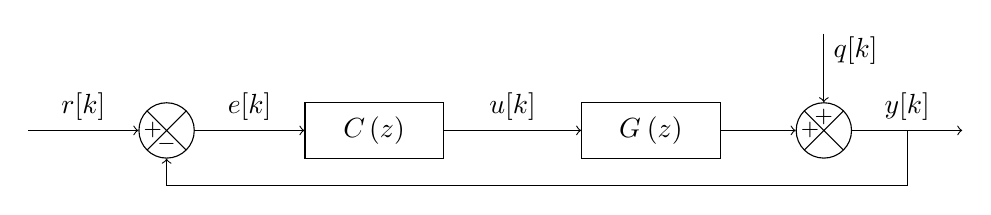
\begin{tikzpicture}[auto, node distance=7.5em]
        \node [input, name=input] {};
        \node [draw, circle, add={$-$}{$+$}{}{}, right of=input, node distance=5em] (sum) {};
        \node [block, right of=sum] (c) {$\myC{z}$};
        \node [block, right of=c, node distance=10em] (g) {$\myG{z}$};
        \node [draw, circle, add={}{$+$}{$+$}{}, right of=g, node distance=6.25em] (sum2) {};
        \node [output, right of=sum2, node distance=5em] (output) {};

        \draw [->] (input) -- node {$r[k]$} (sum);
        \draw [->] (sum) -- node {$e[k]$} (c);
        \draw [->] (c) -- node {$u[k]$} (g);
        \draw [->] (g) -- (sum2);
        \draw [->] (sum2) -- node [name=y] {$y[k]$} (output);

        \node [coordinate, above of=sum2, node distance=3.5em] (q2) {};
        \draw [->] (q2) -- node [pos=0.25] {$q[k]$} (sum2);

        \node [coordinate, below of=c, node distance=2em] (fe) {};
        \draw [-] (y) |- (fe);
        \draw [->] (fe) -| (sum);
    \end{tikzpicture}
    %}%
    \\\sourcecitation{adaptado de \cite{Bazanella2005}}
    \label{fig:feedbackloop}
\end{figure}

A função de transferência do sistema em malha fechada estabelece a relação entre os sinais de referência e de saída como
\begin{equation}\label{eq:T_loop}
    T(z) = \dfrac{ y(z) }{ r(z) } = \dfrac{ \myCG{z}{z} }{ 1 + \myCG{z}{z} }
    \,.
\end{equation}
O efeito da perturbação sobre a saída é expresso pela função de transferência da sensibilidade
\begin{equation}\label{eq:T_loop_qy}
    S(z) = \dfrac{ y(z) }{ q(z) } = \dfrac{ 1 }{ 1 + \myCG{z}{z} }
    \,.
\end{equation}
A saída efetiva é dada então pela soma das contribuições individuais, isto é,
\begin{equation}
    y(z) = T(z) \mycdot r(z) + S(z) \mycdot q(z)
    \,.
\end{equation}

O projeto de um sistema de controle consiste em determinar o controlador que faz com que o sistema em malha fechada apresente determinado comportamento, o que normalmente envolve o desempenho adequado para certos tipos de sinais: seguimento de referências e rejeição de perturbações.
Além disso, é comum também especificar outros critérios, como tempo de resposta e máximo sobrepasso.
Mais informações sobre sistemas de controle podem ser encontradas em \cite{Bazanella2005, Ogata2010}.

\subsection{Estabilidade e Causalidade}

Além dos propósitos já citados, o controle objetiva também garantir a estabilidade do sistema.
Existem diferentes critérios de estabilidade para sistemas dinâmicos.
Este trabalho utiliza o critério de que entradas limitadas produzem sempre saídas limitadas --- \textit{Bounded-Input, Bounded-Output} (BIBO) ---, chamado BIBO-estabilidade.
Doravante, o termo estabilidade refere-se à BIBO-estabilidade.

Considere um sistema genérico representado pela função de transferência
\begin{equation}\label{eq:stability_H}
\begin{gathered}
    H(z) = \dfrac{ N_H(z) }{ D_H(z) }
         = \dfrac{ \sum_{i = 0}^{n_z} \left( b_i \mycdot z^i \right) }{ \sum_{i = 0}^{n_p} \left( a_i \mycdot z^i \right) }
         %= K \mycdot \dfrac{ \prod_{i = 1}^{n_z} (z - z_i) }{ \prod_{i = 1}^{n_p} (z - p_i) }
         = \dfrac{ K \mycdot \prod_{i = 1}^{n_z} (z - z_i) }{ \prod_{i = 1}^{n_p} (z - p_i) }
        \,,
        \\
        \left\{ n_z,\, n_p \in \mathbb{N} \mid n_z \leq n_p \right\}
        \,,\;
        \left\{ a_i,\, b_i,\, K \in \mathbb{R} \mid a_{n_p} = 1 \right\}
        \,,\;
        \left\{ z_i,\, p_i \in \mathbb{C} \right\}
        \,,
\end{gathered}
%\,,
\end{equation}
caracterizada pelos polinômios do numerador $N_H(z)$ e do denominador $D_H(z)$.
Con\-ven\-ci\-o\-na\--se que o polinômico $D_H(z)$ seja mônico.
As raízes de $N_H(z)$ são denominadas zeros da função de transferência, $z_i$, enquanto as raízes de $D_H(z)$ são denominadas polos, $p_i$.
%Os valores dos polos e zeros podem ser repetidos ou até mesmo pares de valores complexos conjugados.

%Para que um sistema seja estável, é necessário e suficiente que todos os seus polos tenham módulo menor que a unidade, ou seja, $\left| p_i \right| < 1,\; \left\{ i \in \mathbb{N} \mid 1 \leq i \leq n_p \right\}$ \cite{Haykin2001}.
Para que um sistema seja estável, é necessário e suficiente que todos os seus polos tenham módulo estritamente menor que a unidade.
Polos de módulo igual a unidade são chamados marginalmente estáveis, enquanto os de módulo maior que a unidade são denominados instáveis.
É comum representar graficamente os polos e zeros de um sistema como localizações em um plano complexo denominado plano $z$, resultando no mapa de polos e zeros.
Nesse caso, diz-se que o sistema é estável se todos os seus polos estiverem no interior de uma circunferência de raio unitário centrada na origem.

O tratamento de sistemas reais implica causalidade, isto é, as saídas dependem dos valores atuais e passados das entradas, e não de valores futuros.
Essa propriedade está associada ao grau relativo do sistema, que pode ser definido como a diferença entre o grau de $D_H(z)$ e o grau de $N_H(z)$, ou ainda como a diferença entre o número de polos $n_p$ e o número de zeros $n_z$.
Sistemas causais devem ter grau relativo não negativo.

\subsection{Princípio do Modelo Interno}\label{sec:controle_PMI}

O Princípio do Modelo Interno (PMI) permite projetar controladores que proporcionam robustez no seguimento de referência e rejeição de perturbações para sinais de classe conhecida.
Este princípio é apresentado detalhadamente em \cite{Chen1999}.

Considere um sinal de referência qualquer, cuja transformada $z$ é
\begin{equation}\label{eq:pmi_r_frac}
    r(z) = \dfrac{ N_r(z) } {D_r(z) } = \dfrac{ N_r(z) }{ \phi_u(z) \mycdot \phi_s(z) }
    \,,
\end{equation}
sendo $D_r(z)$ um polinômio mônico.
Este polinômio pode ser fatorado em outros dois, sendo $\phi_u(z)$ o polinômio cujas raízes representam os modos instáveis --- localizados no exterior do círculo unitário --- e marginalmente estáveis --- sobre o círculo unitário ---, e $\phi_s(z)$ o polinômio que contém os modos estáveis --- no interior do círculo unitário.

Seja
\begin{equation}\label{eq:pmi_G_frac}
    G(z) = \dfrac{ N_G(z) }{ D_G(z) }
\end{equation}
a função de transferência do processo a ser controlado.
Se $\phi_u(z)$ não for um fator de $N_G(z)$, então, pelo PMI, um controlador
\begin{equation}\label{eq:pmi_C_frac}
    C(z) = \dfrac{ N_C(z) }{ D_C(z) } = \dfrac{ N_C(z) }{ \phi_u(z) \mycdot \overline{D_C}(z) }
\end{equation}
é suficiente para proporcionar seguimento da referência, desde que o sistema em malha fechada seja estável.
Diz-se que o controlador implementa o modelo interno da referência.

%Para verificar esse princípio, considere o erro de seguimento do sistema, dado pela Equação \eqref{eq:pmi_e}.
%O valor do erro em regime permanente pode então ser obtido pelo Teorema do Valor Final (TVF).

% \begin{equation}\label{eq:pmi_e}
% \begin{aligned}
    % e(z) &= r(z) - y(z) = r(z) - T(z) \mycdot r(z) \\
         %%&= \dfrac{ D_r(z) \mycdot \overline{D_C}(z) \mycdot D_G(z) }{ D_r(z) \mycdot \overline{D_C}(z) \mycdot D_G(z) + N_C(z) \mycdot N_G(z) } \mycdot \dfrac{ N_r(z) }{ D_r(z) } \\
        %  &= \dfrac{ \overline{D_C}(z) \mycdot D_G(z) }{ D_r(z) \mycdot \overline{D_C}(z) \mycdot D_G(z) + N_C(z) \mycdot N_G(z) } \mycdot N_r(z)
% \end{aligned}
% \end{equation}

% \begin{equation}
    % \lim_{k \to \infty} e[k]
    %% = \lim_{z \to 1} \left(1 - z^{-1} \right) \mycdot e(z)
    % = \lim_{z \to 1} \dfrac{ z - 1 }{ z } \mycdot e(z)
% \end{equation}

Substituindo as equações \eqref{eq:pmi_G_frac} e \eqref{eq:pmi_C_frac} em \eqref{eq:T_loop} obtém-se a função de transferência do sistema em malha fechada:
\begin{equation}\label{eq:pmi_T}
    T(z) = \dfrac{ N_C(z) \mycdot N_G(z) }{ \phi_u(z) \mycdot \overline{D_C}(z) \mycdot D_G(z) + N_C(z) \mycdot N_G(z) }
    \,.
\end{equation}
Observe que a estabilidade pode ser atingida pela escolha adequada de $\overline{D_C}(z)$ e $N_C(z)$.

Para obter a rejeição assintótica de perturbações, basta que o controlador implemente também o modelo interno desses sinais.
Teoricamente, um controlador pode implementar o modelo interno de tantos sinais quanto forem de interesse.
Na prática, porém, a implementação pode ter um limite de complexidade;
além disso, um grande número de parâmetros a sintonizar pode representar uma dificuldade.

%Além do seguimento da referência, o PMI proporciona ainda a rejeição assintótica de perturbações, desde que o controlador implemente também o modelo interno de tais perturbações.
%Mais detalhes, incluindo a prova do princípio, podem ser vistos em \cite{Chen1999}.

\subsubsection{Controlador Proporcional-Ressonante}\label{sec:controle_PR}

Neste trabalho há interesse na resposta à referência e perturbações senoidais.
No tempo discreto, um sinal senoidal com fase nula é expresso por
\begin{equation}\label{eq:ress_ref_k}
    r[k] = A \mycdot \sin \left( \Omega \mycdot k \right)
    \,,
\end{equation}
em que $A$ é a amplitude e $\Omega$ é a frequência discretizada, definida em termos da frequência angular $\omega$ ou frequência $f$ e do período de amostragem $T_s$:
\begin{equation}\label{eq:ress_Omega}
    \Omega = \omega \mycdot T_s = 2 \mycdot \pi \mycdot f \mycdot T_s
    \,.
\end{equation}

A transformada $z$ do sinal \eqref{eq:ress_ref_k} é
\begin{equation}\label{eq:ress_ref_z}
    r(z) = \dfrac{ A \mycdot \sin \left( \Omega \right) \mycdot z }
                 { z^2 - 2 \mycdot \cos \left( \Omega \right) \mycdot z + 1 }
    \,,
\end{equation}
cujas raízes do denominador são um par de valores complexos conjugados de módulo unitário e ângulo $\pm\Omega$, sendo, portanto, marginalmente estáveis.
Assim, pelo PMI, o controlador que proporciona seguimento a esse tipo de referência deve ser da forma
\begin{equation}\label{eq:ress_C_PR}
    \myC[PR]{z}
    %= \dfrac{ k_2 \mycdot z^2 + k_1 \mycdot z + k_0 }
    %        { z^2 - 2 \mycdot \cos \left( \Omega \right) \mycdot z + 1 }
    = \dfrac{ K \mycdot (z - z_1) (z - z_2) }
            { z^2 - 2 \mycdot \cos \left( \Omega \right) \mycdot z + 1 }
    = k_{PR} + \dfrac{ k_{R_1} \mycdot z + k_{R_0} }
                  { z^2 - 2 \mycdot \cos \left( \Omega \right) \mycdot z + 1 }
    \,.
\end{equation}
Essa classe de controlador, denominada Proporcional-Ressonante (PR), permite o ajuste de dois zeros, $z_1$ e $z_2$, e um ganho, $K$, através dos coeficientes $k_{R_0}$, $k_{R_1}$ e $k_{PR}$.
%O par de polos complexos conjugados é posicionado sobre o círculo unitário, fazendo com que a estrutura seja marginalmente estável.
O nome vem do fato de que este controlador apresenta ressonância na frequência $\Omega$, isto é, o ganho do controlador para $z = e^{\pm j \mycdot \Omega}$ tende ao infinito.

\subsubsection{Controlador Proporcional-Múltiplo-Ressonante}\label{sec:controle_PMR}

O controlador PR permite seguir ou rejeitar sinais senoidais de uma única frequência.
Sinais periódicos genéricos podem, através da expansão por séries de Fourier, ser representandos pela sobreposição de senoides de frequências harmônicas \cite{Haykin2001, Kreyszig2014}.
Para atuar sobre esse tipo de sinal, o controlador deve implementar o modelo interno das múltiplas frequências que o compõem.
A aplicação detalhada do PMI para processos periódicos genéricos pode ser vista em \cite{Flores2012}.

A combinação paralela de múltiplos controladores PR resulta no controlador Pro\-por\-ci\-o\-nal-Múl\-ti\-plo-Res\-so\-nan\-te (PMR):
\begin{equation}
\begin{gathered}
    \myC[PMR]{z}
    %= \sum_{i=1}^{n} \myC[PR,i]{z}
    %= \sum_{i=1}^{n} \dfrac{ k_{i,2} \mycdot z^2 + k_{i,1} \mycdot z + k_{i,0} }
    %                       { z^2 - 2 \mycdot \cos \left( \Omega_i \right) \mycdot z + 1 }
    %= K \mycdot \sum_{i=1}^{n} \dfrac{ (z - z_{i_1}) (z - z_{i_2}) }
    %                               { z^2 - 2 \mycdot \cos \left( \Omega_i \right) \mycdot z + 1 }
    = \sum_{i=1}^{n} \dfrac{ K_i \mycdot (z - z_{i_1}) (z - z_{i_2}) }
                           { z^2 - 2 \mycdot \cos \left( \Omega_i \right) \mycdot z + 1 }
    = k_{PR} + \sum_{i=1}^{n} \dfrac{ k_{R_{i_1}} \mycdot z + k_{R_{i_0}} }
                                 { z^2 - 2 \mycdot \cos \left( \Omega_i \right) \mycdot z + 1 }
    \,,
    \\
    \left\{ n \in \mathbb{N} \mid n > 1 \right\}
    \,.
\end{gathered}
\end{equation}
Observe que cada frequência de interesse $\Omega_i$ introduz dois zeros em posições arbitradas e dois polos marginalmente estáveis.
O número de parâmetros a sintonizar equivale a $2 \mycdot n + 1$, em que $n$ é o número de frequências ressonantes.
O controlador PMR apresenta ressonância em cada uma dessas frequências.

Além do seguimento de sinais periódicos genéricos, o controlador PMR pode também ser aplicado em sistemas excitados por sinais senoidais que sofrem de perturbações nas harmônicas desse sinal.
Pela implementação do modelo interno das harmônicas, é possível rejeitar assintoticamente tais perturbações.
Por questões práticas, o controlador pode não conter todas as harmônicas, somente aquelas de maior relevância.

\subsection{\textit{Virtual Reference Feedback Tuning}}\label{sec:VRFT}

A sintonia pela referência virtual realimentada --- \textit{Virtual Reference Feedback Tuning} (VRFT) --- é um método não iterativo baseado em dados utilizado para determinar os parâmetros de um controlador através de um único ensaio.
Este método é inicialmente introduzido para um sistema de controle SISO como aquele da Figura \ref{fig:feedbackloop}, conforme apresentam \textcite{Campi2000}.

%Considere um sistema linear e invariante no tempo --- \textit{Linear Time Invariant} (LTI) --- representado pela função de transferência desconhecida $G(z)$.
Considere um sistema linear e invariante no tempo representado pela função de transferência desconhecida $G(z)$.
Defina um modelo de referência $T_d(z)$ --- isto é, uma função de transferência desejada para o sistema em malha fechada --- e um controlador parametrizado
\begin{equation}\label{eq:VRFT_Czrho}
    \myCzrho{} = \rho \mycdot \myoC[]{z}
    \,,
\end{equation}
em que $\rho$ é um vetor linha de parâmetros e $\myoC[]{z}$ é um vetor coluna de funções de transferência, ambos de mesmo comprimento.
Defina o custo do modelo modelo de referência
\begin{equation}\label{eq:VRFT_Jmr}
\begin{aligned}
    J_{mr} \left( \rho \right)
    &= {\left\lVert W(z) \mycdot \left( T(z, \rho) - T_d(z) \right) \right\rVert_2}^2
    %\\&= {\left\lVert W(z) \mycdot \left( \dfrac{ \myCzrho{} \mycdot G(z) }{ 1 + \myCzrho{} \mycdot G(z) } - T_d(z) \right) \right\rVert_2}^2
    \,,
\end{aligned}
%    \,,
\end{equation}
o qual compara a função de transferência $T(z, \rho)$, obtida com o controlador $\myCzrho{}$ em malha fechada, com a função de transferência desejada, sendo $W(z)$ uma função ponderadora qualquer.
O problema consiste então em encontrar o valor de $\rho$ que minimiza esse custo.

Realize um experimento, em malha aberta ou fechada, para obtenção de sinais de entrada, $u[k]$, e saída, $y[k]$, do processo.
Defina o sinal de referência virtual, $\overline{r}[k]$, como o sinal que, aplicado na função de transferência desejada, resultaria na saída obtida no ensaio, de acordo com
\begin{equation}\label{eq:VRFT_rv}
    y(z) = T_d(z) \mycdot \overline{r}(z)
    \,.
\end{equation}
Defina também o erro virtual
\begin{equation}\label{eq:VRFT_ev}
    \overline{e}[k] = \overline{r}[k] - y[k]
    \,,
\end{equation}
isto é,  a diferença entre a referência virtual e a saída obtida do ensaio.
Esse procedimento é exemplificado pela Figura \ref{fig:VRFT}, em que os sinais e sistemas virtuais são representados por linhas tracejadas.

\begin{figure}[h]
    \centering
    \caption{Diagrama de blocos de um sistema de controle virtual.}
    %\resizebox{\textwidth}{!}{%
    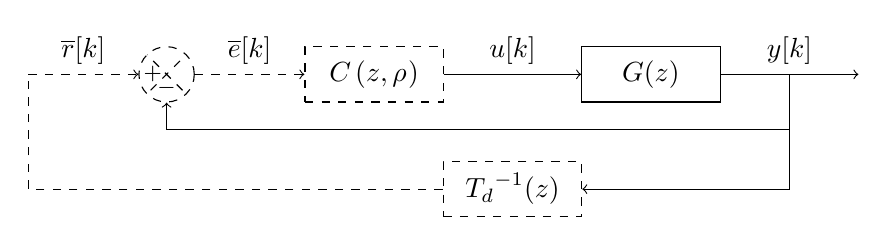
\begin{tikzpicture}[auto, node distance=7.5em]
        \node [block] (G) {$G(z)$};
        \node [output, right of=G, node distance=7.5em] (output) {};

        \node [block, left of=G, node distance=10em, dashed] (C) {$\myCzrho{}$};
        \node [draw, circle, add={$-$}{$+$}{}{}, left of=C, dashed] (sum) {};
        \node [input, left of=sum, node distance=5em] (input) {};

        \draw [->] (G) -- node [name=y] {$y[k]$} (output);
        \draw [->] (C) -- node [name=u] {$u[k]$} (G);
        \draw [->, dashed] (sum) -- node {$\overline{e}[k]$} (C);

        \node [coordinate, below of=C, node distance=2em] (fe) {};
        \draw [-] (y) |- (fe);
        \draw [->] (fe) -| (sum);

        \node [block, below of=u, node distance=5em, dashed] (Td) {${T_d}^{-1}(z)$};
        \draw [->] (y) |- (Td);
        \draw [-, dashed] (Td) -| (input);
        \draw [->, dashed] (input) -- node {$\overline{r}[k]$} (sum);
    \end{tikzpicture}
    %}%
    \\\sourcecitation{adaptado de \cite{Chrystian2020}}
    \label{fig:VRFT}
\end{figure}

Defina agora o custo de referência virtual
\begin{equation}\label{eq:VRFT_Jvr}
\begin{aligned}
    J_{vr} \left( \rho \right)
    &= {\left\lVert L(z) \mycdot \left( u(z) - \overline{u}(z) \right) \right\rVert_2}^2\\
    %&= {\left\lVert L(z) \mycdot \left( u(z) - \myCzrho{} \mycdot \overline{e}(z) \right) \right\rVert_2}^2\\
    &= {\left\lVert L(z) \mycdot \left( u(z) - \rho \mycdot \myoC[]{z} \mycdot \overline{e}(z) \right) \right\rVert_2}^2
    \,,
\end{aligned}
    %\,,
\end{equation}
que compara o sinal efetivamente aplicado no processo durante o ensaio com o sinal que seria produzido pelo controlador a partir do erro virtual, sendo $L(z)$ um filtro ponderador.
Em condições ideais, a obtenção do valor de $\rho$ que minimiza esse custo é análoga a minimização do custo do modelo de referência.

Defina o vetor de regressão
\begin{equation}\label{eq:VRFT_phi}
    \varphi(z) = \myoC{z} \mycdot \overline{e}(z) = \myoC{z} \mycdot \left( {T_d}^{-1}(z) - 1 \right) \mycdot y(z)
    \,.
\end{equation}
Então, substituindo a Equação \eqref{eq:VRFT_phi} em \eqref{eq:VRFT_Jvr}, o custo de referência virtual pode ser reescrito como
\begin{equation}\label{eq:VRFT_Jvr_2}
    J_{vr} \left( \rho \right)
    = {\left\lVert L(z) \mycdot \left( u(z) - \rho \mycdot \varphi(z) \right) \right\rVert_2}^2
    \,.
\end{equation}
Essa equação é quadrática em $\rho$, o que garante a existência de um mínimo global.
%Ademais, a minimização pode ser realizada por uma fórmula fechada.
%O valor de $\rho$ que leva a esse mínimo pode ser, inclusive, obtido através de uma fórmula fechada.

%Se os dados coletados no ensaio forem livres de ruído e o controlador ideal --- isto é, aquele que efetivamente resulta na função de transferência desejada --- pertencer a classe de controladores definida pelo vetor $\myoC[]{z}$, então os custos $J_{mr}(\rho)$ e $J_{vr}(\rho)$ são idênticos e o mínimo de ambos é zero, portanto o controlador ideal pode ser obtido.
Se os dados coletados no ensaio forem livres de ruído e o controlador ideal --- isto é, aquele que efetivamente resulta na função de transferência desejada --- pertencer a classe de controladores definida pelo vetor $\myoC[]{z}$, então os custos $J_{mr}(\rho)$ e $J_{vr}(\rho)$ são idênticos e, portanto, o controlador ideal pode ser obtido.
Na prática, porém, há presença de ruído e o controlador ideal pode não ser atingível através de $\myoC[]{z}$.

A fim de obter o controlador sub-parametrizado que melhor aproxima a função de transferência desejada em malha fechada, o filtro $L(z)$ aproxima o mínimo de $J_{vr}(\rho)$ ao mínimo de $J_{mr}(\rho)$.
O filtro ideal é obtido ao aplicar o Teorema de Parseval nas equações \eqref{eq:VRFT_Jmr} e \eqref{eq:VRFT_Jvr} e igualá-las.
Após algumas aproximações, obtém-se
\begin{equation}\label{eq:VRFT_L}
    L(z) = T_d(z) \mycdot \left( 1 - T_d(z) \right)
    \,.
\end{equation}
O procedimento completo é demonstrado por \textcite{Campi2000, Bazanella2011}.

Alguns fatores devem ser considerados pelo projetista na aplicação do método VRFT.
As escolhas da função de transferência desejada, da classe do controlador e do sinal aplicado no ensaio afetam diretamente os resultados obtidos.
A estabilidade do sistema com o controlador obtido deve ser avaliada, visto que o VRFT não a garante.
%Além disso, sob determinadas condições, a presença de ruído no sistema pode ser minimizada pela realização de dois ensaios sob um mesmo sinal, os quais são combinados para determinação do controlador.
%Esses e outros detalhes podem ser explorados em \cite{Campi2000} e \cite{Bazanella2011}.
Esses e outros detalhes são explorados por \textcite{Bazanella2011}.

\subsubsection{Sistemas em Cascata com Controlador Interno no Laço de Realimentação}\label{sec:VRFT_cascata}

\textcite{Chrystian2020} estendem o método VRFT para sistemas de controle SISO com topologia em cascata.
Considere a estrutura de controle apresentada na Figura \ref{fig:cascadeloop1}, em que os sinais $u[k]$, $y_i[k]$ e $y_e[k]$ são mensuráveis.
Deseja-se sintonizar, simultaneamente, os controladores externo $\myCzrho{e}$ e interno $\myCzrho{i}$, os quais estão parametrizados em função de $\rho_e$ e $\rho_i$, respectivamente.
A função de transferência desse sistema em malha fechada é
\begin{equation}\label{eq:VRFT_cascade1_T}
    \myT{z, \rho_e, \rho_i} =
        \frac{ \myC[e]{z, \rho_e} \mycdot \myG[i]{z} \mycdot \myG[e]{z} }
             {1 + \myCG[i]{z, \rho_i}{z} + \myC[e]{z, \rho_e} \mycdot \myG[i]{z} \mycdot \myG[e]{z} }
    \,.
\end{equation}

\begin{figure}[h]
    \centering
    \caption{Diagrama de blocos de um sistema de controle SISO em cascata com controlador interno no laço de realimentação.}
    \resizebox{\textwidth}{!}{%
    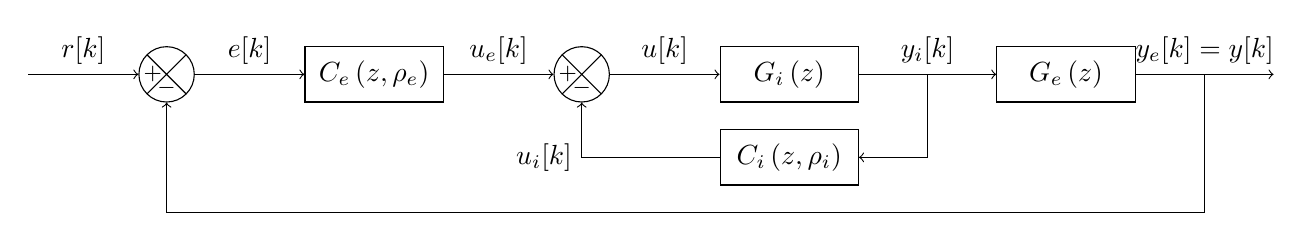
\begin{tikzpicture}[auto, node distance=7.5em]
        \node [input, name=input] {};
        \node [draw, circle, add={$-$}{$+$}{}{}, right of=input, node distance=5em] (sum1) {};
        \node [block, right of=sum1] (ce) {$\myCzrho{e}$};
        \node [draw, circle, add={$-$}{$+$}{}{}, right of=ce] (sum2) {};
        \node [block, right of=sum2] (gi) {$\myG[i]{z}$};
        \node [block, right of=gi, node distance=10em] (ge) {$\myG[e]{z}$};
        \node [output, right of=ge, node distance=7.5em] (output) {};

        \node [block, below of=gi, node distance=3em] (ci) {$\myCzrho{i}$};

        \draw [->] (input) -- node {$r[k]$} (sum1);
        \draw [->] (sum1) -- node {$e[k]$} (ce);
        \draw [->] (ce) -- node {$u_e[k]$} (sum2);
        \draw [->] (sum2) -- node {$u[k]$} (gi);
        \draw [->] (gi) -- node [name=yi] {$y_i[k]$} (ge);
        \draw [->] (ge) -- node [name=y] {$y_e[k] = y[k]$} (output);

        \draw [->] (yi) |- (ci);
        \draw [->] (ci) -| node {$u_i[k]$} (sum2);

        \node [coordinate, below of=ci, node distance=2em] (fe) {};
        \draw [-] (y) |- (fe);
        \draw [->] (fe) -| (sum1);
    \end{tikzpicture}
    }%
    \\\sourcecitation{adaptado de \cite{Chrystian2020}}
    \label{fig:cascadeloop1}
\end{figure}

\newpage
O custo de referência virtual é redefinido para considerar a contribuição de ambos os controladores:
\begin{equation}\label{eq:VRFT_cascade1_Jvr}
\begin{aligned}
    J_{vr} \left( \rho_e, \rho_i \right)
    %&= {\left\lVert L(z) \mycdot \left( u(z) - \overline{u}(z) \right) \right\rVert_2}^2\\
    &= {\left\lVert L(z) \mycdot \left( u(z) - \left( \overline{u_e}(z) - \overline{u_i}(z) \right) \right) \right\rVert_2}^2\\
    %&= {\left\lVert L(z) \mycdot \left( u(z) - \left( \myCzrho{e} \mycdot \overline{e}(z) - \myCzrho{i} \mycdot y_i(z) \right) \right) \right\rVert_2}^2
    &= {\left\lVert L(z) \mycdot \left( u(z) - \left( \rho_e \mycdot \myoC[e]{z} \mycdot \overline{e}(z) - \rho_i \mycdot \myoC[i]{z} \mycdot y_i(z) \right) \right) \right\rVert_2}^2
    %&= {\left\lVert L(z) \mycdot \left( u(z) - \left( \myCzrho{e} \mycdot \left( {T_d}^{-1}(z) - 1 \right) \mycdot y_e(z) - \myCzrho{i} \mycdot y_i(z) \right) \right) \right\rVert_2}^2
    \,.
\end{aligned}
%\,.
\end{equation}
Redefine-se também o vetor de parâmetros
\begin{equation}\label{eq:VRFT_cascade1_rho}
    \rho = \begin{bmatrix} \rho_e && \rho_i \end{bmatrix}
    %\,
\end{equation}
e o vetor de regressão
\begin{equation}\label{eq:VRFT_casdade1_phi}
    \varphi(z)
    =
    \begin{bmatrix}
        \myoC[e]{z} \mycdot \overline{e}(z)
        \\
        - \myoC[i]{z} \mycdot y_i(z)
    \end{bmatrix}
    =
    \begin{bmatrix}
        \myoC[e]{z} \mycdot \left( {T_d}^{-1}(z) - 1 \right) \mycdot y_e(z)
        \\
        - \myoC[i]{z} \mycdot y_i(z)
    \end{bmatrix}
    %\,
\end{equation}
de modo a aglutinar as variáveis das malhas externa e interna.
Aplicando \eqref{eq:VRFT_cascade1_rho} e \eqref{eq:VRFT_casdade1_phi} em \eqref{eq:VRFT_cascade1_Jvr}, o custo de referência virtual volta a ter exatamente o formato da Equação \eqref{eq:VRFT_Jvr_2}, a qual é quadrática em $\rho$.

A determinação do filtro $L(z)$ dessa vez depende não apenas da função de transferência desejada para o sistema em malha fechada, mas também do controlador e processo internos.
Utilizando a função de transferência da sensibilidade interna
\begin{equation}\label{eq:VRFT_cascade1_S}
    S_i(z, \rho_i) = \dfrac{ 1 }{ 1 + \myCzrho{i} \mycdot \myG[i]{z} }
    \,,
\end{equation}
o filtro é redefinido como
\begin{equation}\label{eq:VRFT_cascade1_L}
    L(z) = S_i(z, \rho_i) \mycdot T_d(z) \mycdot \left( 1 - T_d(z) \right)
    \,.
\end{equation}

Observe que $S_i(z, \rho_i)$ depende do processo, cuja dinâmica é considerada desconhecida, e, portanto, não pode ser determinada diretamente.
Assim, \textcite{Chrystian2020} propõem um procedimento que permite aproximá-la iterativamente.
Note que, apesar desse processo ser iterativo, apenas um conjunto de dados é necessário.
O método é replicado a seguir:
\begin{enumerate}
    \item Minimize o custo de referência virtual, $J_{vr} \left( \rho_e, \rho_i \right)$, para um filtro $L(z)$ obtido a partir de uma estimativa inicial para $S_i(z, \rho_i)$. Se nenhuma estimativa inicial for conhecida, utilize  $S_i(z, \rho_i) = 1$, equivalente ao caso sem realimentação interna.
    \item Determine o sinal $\overline{u_e}(z) = u(z) + \myCzrho{i} \mycdot y_i(z)$ a partir do $\rho_i$ obtido no passo anterior. Então, estime $S_i(z, \rho_i)$ pela relação $S_i(z, \rho_i) = \frac{u(z)}{\overline{u_e}(z)}$.
    \item Minimize o custo de referência virtual, $J_{vr} \left( \rho_e, \rho_i \right)$, para um filtro $L(z)$ obtido a partir de $S_i(z, \rho_i)$ estimado no passo 2. Repita os passos 2 e 3 até $\rho$ convergir.
\end{enumerate}

\newpage
\section{Fonte de Alimentação Ininterrupta}\label{sec:UPS}

% TODO revisar pra não ficar repetitivo com a introdução
% Praticamente todo o o conteúdo aqui veio do Rashid. Cito só no final? No início? Várias vezes?

A fonte de alimentação ininterrupta --- \textit{Uninterruptible Power Supply} (UPS) --- é um sistema de potência capaz de fornecer alimentação elétrica ininterrupta, confiável e de alta qualidade, conectado entre a rede elétrica e dispositivos críticos ou sensíveis.
Através de uma reserva de energia, a UPS é capaz de, em caso de falha da rede, imediatamente suprir a alimentação, mantendo equipamentos em funcionamento por certo tempo.
Além disso, a UPS atua na atenuação de perturbações na rede, como quedas e pico de tensão e distorções harmônicas.
%Aplicações típicas de UPSs incluem instalações hospitalares, armazenamento de dados, equipamentos de emergência e sistemas de telecomunicação \cite{Rashid2011}. % Já está na introdução

Dentre as características desejáveis para uma UPS, citam-se:
fornecimento de uma tensão senoidal regulada de baixa distorção harmônica;
rápido suprimento da alimentação em caso de falha na rede;
%baixa distorção harmônica na corrente;
fator de potência unitário;
alta eficiência;
e isolamento elétrico
\cite{Rashid2011}.
Diferentes configurações de UPSs enfatizam alguns desses aspectos.

Este trabalho tem como objeto de estudo uma UPS monofásica de topologia \textit{online}, também denominada de dupla-conversão.
A Figura \ref{fig:UPS-online} ilustra essa configuração.
A UPS \textit{online} permanece continuamente em atuação, mesmo quando não há falha na rede.
Sua principal vantagem é o rápido tempo de resposta a alterações, além de bom condicionamento do sinal.
%As desvantagens incluem baixo fator de potência, alta distorção harmônica na entrada e baixa eficiência \cite{Rashid2011}.
As desvantagens incluem baixo fator de potência, alta distorção harmônica e baixa eficiência \cite{Rashid2011}.

\begin{figure}[h]
    \centering
    \caption{Diagrama estrutural de uma UPS \textit{online}.}
    \resizebox{0.8\textwidth}{!}{%
    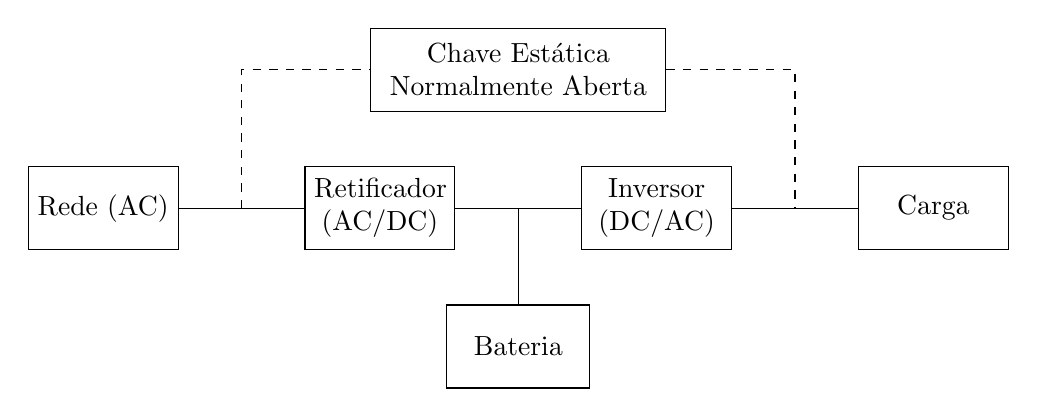
\begin{tikzpicture}[auto, node distance=10em]
        \node [block, minimum height=3em, text width=4.75em, align=center] (ac) {Rede (AC)};
        \node [block, minimum height=3em, text width=4.75em, align=center, right of=ac] (acdc) {Retificador (AC/DC)};
        \node [block, minimum height=3em, text width=4.75em, align=center, right of=acdc] (dcac) {Inversor (DC/AC)};
        \node [block, minimum height=3em, text width=4.75em, align=center, right of=dcac] (load) {Carga};

        \draw[-] (ac)   -- node[coordinate] (med1) {} (acdc);
        \draw[-] (acdc) -- node[coordinate] (med2) {} (dcac);
        \draw[-] (dcac) -- node[coordinate] (med3) {} (load);

        \node [block, minimum height=3em, text width=4.5em, align=center, below of=med2, node distance = 5em] (battery) {Bateria};
        \node [block, minimum height=3em, text width=10em , align=center, above of=med2, node distance = 5em] (switch) {Chave Estática Normalmente Aberta};

        \draw[-] (med2) -- node {} (battery);

        \draw[dashed] (med1) |- node {} (switch);
        \draw[dashed] (switch) -| node {} (med3);
    \end{tikzpicture}
    }%
    \\\sourcecitation{adaptado de \cite{Rashid2011}}
    \label{fig:UPS-online}
\end{figure}

No estágio de entrada, a alimentação provinda da rede elétrica como AC é retificada para DC.
No estágio de saída, a carga é alimentada por um inversor, o qual realiza nova conversão, desta vez de DC para AC.
Uma bateria entre os conversores armazena a reserva de energia, a qual é utilizada em caso de falha da rede.
Pode haver ainda uma chave para conexão direta entre a rede e a carga, a qual permanece aberta em condições normais de operação.

Em particular, o foco deste trabalho está no estágio de saída.
Os demais componentes estão fora do escopo do trabalho e, portanto, não serão detalhados.

A Figura \ref{fig:UPS-electrical} mostra o modelo do circuito elétrico do estágio de saída de uma UPS \textit{online} monofásica, com inversor em meia ponte.
%Considera-se que a tensão $V_{DC}$, fornecida pela bateria e estabilizada pelos capacitores $C_1$ e $C_2$ é constante.
A bateria fornece uma tensão DC aproximadamente constante $V_{DC}$, a qual é estabilizada pelos capacitores $C_1$ e $C_2$.
O inversor é composto pelos transistores bipolares de porta isolada --- \textit{Insulated Gate Bipolar Transistor} (IGBT) --- $S_1$ e $S_2$, os quais são alternadamente acionados por modulação por largura de pulso --- \textit{Pulse Width Modulation} (PWM).
%O PWM senoidal é obtido através da comparação entre um sinal de atuação $v_u$ com uma onda triangular $v_{tri}$.
O PWM é obtido através da comparação entre um sinal de atuação $u$ com uma onda triangular $v_{tri}$.
Como esse acionamento gera uma forma de onda descontínua, é aplicado um filtro indutivo-capacitivo (LC), composto por um indutor, de indutância $L_f$ e resistência interna $R_{L_f}$, e um capacitor, de capacitância $C_f$.
A carga costuma ser representada por sua admitância $Y_o$, a qual pode ser variável e não linear.
%Distúrbios de corrente são representados pela fonte $i_d$.
O principal sinal de interesse é a tensão sobre a carga $v_o$.
A corrente no indutor $i_{L_f}$ também é monitorada.

\begin{figure}[h]
    \centering
    \caption{Circuito elétrico do estágio de saída da UPS.}

    \resizebox{\textwidth}{!}{
    \begin{circuitikz}
        \draw (0,0) node[op amp, /tikz/circuitikz/bipoles/length=0.85cm, yscale=-1](comparator){}; % Comparator
        %\draw (comparator.center) node[schmitt symbol]{};
        \draw (comparator.-) -- ++(0,-0.25) to [vsourcetri, l_=$v_{tri}(t)$] ++(0,-1.5) node[sground]{}; % Triangular source + Signal Ground
        %\draw (comparator.+) node[ocirc, label=left:$v_u(t)$](){}; % v_u(t)
        \draw (comparator.+) node[ocirc, label=left:$u(t)$](){}; % u(t)
        \draw (comparator.out) to [short, *-] ++(0,-1.5) -- ++(0.25,0) node[not port, anchor=in, /tikz/circuitikz/bipoles/length=.85cm](not){}; % NOT Gate
        \draw (not.out) node[nigbt, anchor=B, bodydiode, /tikz/circuitikz/bipoles/length=2cm](s2){$S_2$} % S2 IGBT
            ++(0,3) node[nigbt, anchor=B, bodydiode, /tikz/circuitikz/bipoles/length=2cm](s1){$S_1$}; % S1 IGBT, positioned in relation to S2
        \draw (comparator.out) |- (s1.B); % short comparator out to S1 base
        \draw (s2.E) |- ++(-6.25,-0.25) coordinate (C2Bottom); % short S2.E to C2Bottom Coord
        \draw (C2Bottom) to [short, *-] ++(0,0.5) to [capacitor, l=$C_2$] ++(0,1.5) \pgfextra{\pgfgetlastxy{\xlast}{\ylast}} to [short, -*] (\xlast,0) coordinate (Ground); % C2 + Ground Coord
        \draw (Ground) to [short] +(-0.5,0) node[ground, /tikz/circuitikz/bipoles/length=2.5cm]{}; % Ground
        \draw (s1.C) |- ++ (-6.25,0.25) coordinate (C1Top); % S1.C to C1Top Coord
        \draw (C1Top) to [short, *-] ++(0,-0.5) to [capacitor, l_=$C_1$] ++(0,-1.5) -- (Ground); % C1
        \draw (C1Top) -- ++(-2.25,0) to [battery, l=$V_{DC}$] ++(0,-5.53) |- (C2Bottom); % V_{DC}
        \draw (s2.C) \pgfextra{\pgfgetlastxy{\xlast}{\ylast}} to [short, -*] (\xlast,0) coordinate (s1s2); %S1-S2 node
        \draw (s1.E) -- (s1s2);  %S1-S2 node
        \draw (s1s2) -- ++(1.75,0) to [resistor, l_=$R_{L_f}$] ++(1,0) to [short, f^=$i_{L_f}(t)$] ++(0.5,0) to [inductor, l_=$L_f$] ++(1,0) to [short, -*] ++(0.5,0) coordinate (Vout); % R_{L_f} + L_f + Vout Coord
        \draw (Vout) to [capacitor, l_=$C_f$, v^=$v_o(t)$] ++(0,-2.5) node[tlground, /tikz/circuitikz/bipoles/length=2cm]{}; % C_f + ground
        \draw (Vout) to [short, -] ++(3,0) coordinate (Load);  % Load Coord
        \draw (Load) to [generic, l_=$\frac{1}{Y_o(t)}$] ++(0,-2.5) node[tlground, /tikz/circuitikz/bipoles/length=2cm]{}; % Y_o + ground

        %boxes
        \draw  (-6.2,-3) node[draw=gray, fill=gray, thick, opacity=0.1, rectangle, anchor=south west, minimum width=3.45cm, minimum height=6cm, label=Bateria (DC)]{};
        \draw  (-2.5,-3) node[draw=gray, fill=gray, thick, opacity=0.1, rectangle, anchor=south west, minimum width=6.55cm, minimum height=6cm, label=Inversor (DC/AC)]{};
        \draw  (4.3,-3) node[draw=gray, fill=gray, thick, opacity=0.1, rectangle, anchor=south west, minimum width=4.9cm, minimum height=4cm, label=Filtro LC]{};
        \draw  (9.45,-3) node[draw=gray, fill=gray, thick, opacity=0.1, rectangle, anchor=south west, minimum width=1.8cm, minimum height=4cm, label=Carga]{};
    \end{circuitikz}
    }%
    \\\sourcecitation{adaptado de \cite{Lorenzini2019}}
    \label{fig:UPS-electrical}
\end{figure}

\subsection{Avaliação de Desempenho}

O desempenho de uma UPS é avaliado pela sua capacidade de fornecer uma tensão senoidal com amplitude e frequência constantes e baixo conteúdo harmônico, mesmo sob variação da carga e distúrbios na rede.
A norma \textcite{IEC62040-3:2011} determina os critérios técnicos de conformidade.
As informações descritas a seguir baseiam-se nesse documento.
Os testes são realizados com as cargas especificadas, mostradas na Figura \ref{fig:UPS_load}.

\begin{figure}[h]
    \centering
    \caption{Cargas para testes em UPS de potência nominal inferior a $4 \text{ kVA}$.}
    \begin{subfigure}[t]{.25\linewidth}
        \centering
        \caption{Carga linear.}
        %\vspace{0.5cm}
        %\resizebox{\textwidth}{!}{
        \begin{circuitikz}[scale=0.9]
            \draw (0,0) node[ocirc, label=$v_o(t)$](){} to [short, -*] (0,-0.5);
            \draw (0,-0.5) -- (1,-0.5) to [switch] ++(0,-1.5) to [resistor, l=$R_{l2}$] ++(0,-1.5) -- ++(-1,0);
            \draw (0,-0.5) -- (-1,-0.5) to [switch] ++(0,-1.5) to [resistor, l=$R_{l1}$] ++(0,-1.5) -- ++(1,0) coordinate (ground);
            \draw (ground) to [short, *-] +(0,-0.5) to ++(0,0) node[tlground, /tikz/circuitikz/bipoles/length=2cm]{};
        \end{circuitikz}
        %}%
        \label{fig:UPS_load_linear}
    \end{subfigure}
    \hfill
    \begin{subfigure}[t]{.74\linewidth}
        \centering
        \caption{Carga não linear.}
        %\resizebox{\textwidth}{!}{
        \begin{circuitikz}[scale=0.9]
            \draw (0,0) node[ocirc, label=left:$v_o(t)$](){} to [short, -*] ++(0.5,0) -- ++(0,1.7) to [switch] ++(1.5,0) to [resistor, l_=$R_{s1}$] ++(1.5,0) to [short, -*] ++(0.5,0) coordinate(RS1) to [diode] ++(0,1.5) to [short, -*] ++(1,0) to [short, -*] ++(1.5,0) coordinate(capacitor1) -- ++(1.5,0) to [resistor, l=$R_{nl1}$] ++(0,-3) to [short, -*] ++(-1.5,0) to [short, -*] ++(-1.5,0) coordinate(d1) -- ++(-1,0) to [diode] (RS1);
            \draw (capacitor1) to [capacitor, l=$C_{nl1}$] ++(0,-3);
            \draw (d1) to [diode, -*] ++(0,1.5) coordinate (g1) to [diode] ++(0,1.5);
            \draw (g1) -- ++(0.5,0) node[tlground, /tikz/circuitikz/bipoles/length=2cm, rotate=90]{};

            \draw (0.5,0) -- ++(0,-1.7) to [switch] ++(1.5,0) to [resistor, l_=$R_{s2}$] ++(1.5,0) to [short, -*] ++(0.5,0) coordinate(RS2) to [diode] ++(0,1.5) to [short, -*] ++(1,0) to [short, -*] ++(1.5,0) coordinate(capacitor2) -- ++(1.5,0) to [resistor, l=$R_{nl2}$] ++(0,-3) to [short, -*] ++(-1.5,0) to [short, -*] ++(-1.5,0) coordinate(d2) -- ++(-1,0) to [diode] (RS2);
            \draw (capacitor2) to [capacitor, l=$C_{nl2}$] ++(0,-3);
            \draw (d2) to [diode, -*] ++(0,1.5) coordinate (g2) to [diode] ++(0,1.5);
            \draw (g2) -- ++(0.5,0) node[tlground, /tikz/circuitikz/bipoles/length=2cm, rotate=90]{};
        \end{circuitikz}
        %}%
        \label{fig:UPS_load_nonlinear}
    \end{subfigure}
    \\\vspace{0.25cm}\sourcecitation{adaptado de \cite{Lorenzini2015}}
    \label{fig:UPS_load}
\end{figure}

A carga linear, exibida na Figura \ref{fig:UPS_load_linear}, é composta por dois resistores em paralelo.
Os resistores devem ser determinados de modo a corresponder a $20 \%$ e $80 \%$ da potência ativa nominal da UPS.
As chaves permitem variar a carga durante a operação.

% \begin{figure}[h]
%     \centering
%     \caption{Carga linear para testes na UPS.}
%     %\resizebox{\textwidth}{!}{
%     \begin{circuitikz}
%         \draw (0,0) node[ocirc, label=left:$v_o(t)$](){} to [short, -*] (0,-1);
%         \draw (0,-1) -- (1,-1) to [switch] ++(0,-1.5) to [resistor, l_=$R_{l1}$] ++(0,-1.5) -- ++(-1,0);
%         \draw (0,-1) -- (-1,-1) to [switch] ++(0,-1.5) to [resistor, l_=$R_{l2}$] ++(0,-1.5) -- ++(1,0) coordinate (ground);
%         \draw (ground) to [short, *-] +(0,-1) to ++(0,0) node[tlground, /tikz/circuitikz/bipoles/length=2cm]{};
%     \end{circuitikz}
%     %}%
%     \\\sourcecitation{adaptado de \cite{Lorenzini2019}}
%     \label{fig:UPS_load_linear}
% \end{figure}

A Figura \ref{fig:UPS_load_nonlinear} apresenta a carga não linear para UPSs cuja potência nominal é inferior a $4 \text{ kVA}$.
Essa carga é composta por dois circuitos independentes, cada um deles com um resistor de entrada, uma ponte retificadora, e um filtro resistivo-capacitivo (RC) paralelo.
Os circuitos devem ser projetados para corresponder a $25 \%$ e $75 \%$ da potência aparente nominal da UPS, e fator de potência $0,7$ atrasado.
Novamente, as chaves permitem variar a carga durante a operação.
Quando excitada por uma tensão senoidal, essa carga causa perturbações nas harmônicas ímpares da frequência de excitação, principalmente da 3{\textordfeminine} até a 9{\textordfeminine} \cite{Pereira2014, Bertoldi2019}.

% \begin{figure}[h]
%     \centering
%     \caption{Carga não linear para testes em UPS de potência nominal inferior a $4 \text{ kVA}$.}
%     %\resizebox{\textwidth}{!}{
%     \begin{circuitikz}
%         \draw (0,0) node[ocirc, label=left:$v_o(t)$](){} to [short, -*] ++(1,0) -- ++(0,2) to [switch] ++(1.5,0) to [resistor, l_=$R_{s1}$] ++(1.5,0) to [short, -*] ++(0.5,0) coordinate(RS1) to [diode] ++(0,1.5) to [short, -*] ++(1,0) to [short, -*] ++(1.5,0) coordinate(capacitor1) -- ++(1.5,0) to [resistor, l=$R_{nl1}$] ++(0,-3) to [short, -*] ++(-1.5,0) to [short, -*] ++(-1.5,0) coordinate(d1) -- ++(-1,0) to [diode] (RS1);
%         \draw (capacitor1) to [capacitor, l=$C_{nl1}$] ++(0,-3);
%         \draw (d1) to [diode, -*] ++(0,1.5) coordinate (g1) to [diode] ++(0,1.5);
%         \draw (g1) -- ++(0.5,0) node[tlground, /tikz/circuitikz/bipoles/length=2cm, rotate=90]{};

%         \draw (1,0) -- ++(0,-2) to [switch] ++(1.5,0) to [resistor, l_=$R_{s2}$] ++(1.5,0) to [short, -*] ++(0.5,0) coordinate(RS2) to [diode] ++(0,1.5) to [short, -*] ++(1,0) to [short, -*] ++(1.5,0) coordinate(capacitor2) -- ++(1.5,0) to [resistor, l=$R_{nl2}$] ++(0,-3) to [short, -*] ++(-1.5,0) to [short, -*] ++(-1.5,0) coordinate(d2) -- ++(-1,0) to [diode] (RS2);
%         \draw (capacitor2) to [capacitor, l=$C_{nl2}$] ++(0,-3);
%         \draw (d2) to [diode, -*] ++(0,1.5) coordinate (g2) to [diode] ++(0,1.5);
%         \draw (g2) -- ++(0.5,0) node[tlground, /tikz/circuitikz/bipoles/length=2cm, rotate=90]{};
%     \end{circuitikz}
%     %}%
%     \\\sourcecitation{adaptado de \cite{Lorenzini2019}}
%     \label{fig:UPS_load_nonlinear}
% \end{figure}

Em regime permanente, a tensão eficaz de saída deve permanecer na faixa de $\pm 10 \%$ de seu valor nominal.
A frequência desse sinal, por sua vez, pode apresentar uma variação de $\pm 2 \%$ a partir do valor nominal.
A máxima distorção harmônica total --- \textit{Total Harmonic Distortion} (THD) --- da tensão é de $8 \%$, enquanto os valores para as distorções harmônicas individuais --- \textit{Individual Harmonic Distortions} (IHD) --- são enumerados na Tabela \ref{tab:IEC_IHD}.

\begin{table}[h]
    \newcolumntype{C}[1]{>{\centering\arraybackslash}b{#1}}
    \centering
    \caption{Máximas distorções harmônicas individuais admissíveis em UPS de baixa tensão.}
    \resizebox{\textwidth}{!}{
    \begin{tabular}{C{0.135\linewidth}|C{0.175\linewidth}|C{0.135\linewidth}|C{0.105\linewidth}|C{0.135\linewidth}|C{0.175\linewidth}}
        \multicolumn{2}{C{0.34\linewidth}|}{\textbf{Harmônicas ímpares não múltiplas de 3}} & \multicolumn{2}{C{0.26\linewidth}|}{\textbf{Harmônicas ímpares múltiplas de 3}} & \multicolumn{2}{C{0.31\linewidth}}{\textbf{Harmônicas pares}} \\ \hline
        \textbf{Ordem ($i$)} & \textbf{IHD [$\%$]}              & \textbf{Ordem ($i$)} & \textbf{IHD [$\%$]}            & \textbf{Ordem ($i$)} & \textbf{IHD [$\%$]}               \\ \hline
        $5 $                 & $6$                              & $3$                  & $5$                            & $2$                  & $2$                               \\ \hline
        $7 $                 & $5$                              & $9$                  & $1,5$                          & $4$                  & $1$                               \\ \hline
        $11$                 & $3,5$                            & $15$                 & $0,3$                          & $6$                  & $0,5$                             \\ \hline
        $13$                 & $3$                              & $21$                 & $0,2$                          & $8$                  & $0,5$                             \\ \hline
        $17 \leq i \leq 49$  & $2,27 \mycdot \frac{17}{i} - 0,27$ & $21 \leq i \leq 45$  & $0,2$                          & $10 \leq i \leq 50$  & $0,25 \mycdot \frac{10}{i} + 0,25$
    \end{tabular}
    }%
    \\\vspace{0.25cm}\sourcecitation{adaptado de \apud{IEC62040-3:2011}{Lorenzini2015}}
    \label{tab:IEC_IHD}
\end{table}

O desempenho transitório é avaliado sob três situações: alteração no modo de operação; variação da carga linear; e variação da carga não linear.
Neste trabalho, apenas os dois último serão verificados.
A norma define três perfis, cada um associado a um envelope de variação de tensão após a alteração.
A Figura \ref{fig:IEC_DynamicVoltage1} mostra o perfil mais rigoroso, para cargas críticas sensíveis.
O desvio de tensão é determinado pela comparação do sinal obtido após o evento com o que seria observado caso o sistema permanecesse inalterado, e a porcentagem é calculada em relação ao valor de pico.

\begin{figure}[h]
    \centering
    \caption{Tensão de saída admissível em regime transitório para cargas críticas sensíveis.}
    \includegraphics[trim={0 0 0 10}, clip, width=0.8\textwidth]{fig/DynamicVoltage1}
    \label{fig:IEC_DynamicVoltage1}
    \\\sourcecitation{\apud{IEC62040-3:2011}{Lorenzini2015}}
\end{figure}

Nos testes de variação da carga, as alterações devem ocorrer no momento em que a tensão de saída estiver em seu valor de pico.
Inicialmente, a UPS deve atingir o regime permanente com a menor carga --- $20 \%$ para o caso linear e $25 \%$ para o caso não linear.
Um degrau aditivo deve então ocorrer, elevando a carga para $100 \%$.
Após atingir novo regime permanente, o degrau subtrativo é aplicado, retornando a carga a seu valor inicial.


\chapter{Metodologia}\label{sec:metodologia}

Este capítulo apresenta a metodologia empregada no desenvolvimento deste trabalho.
Inicialmente, é descrito o ambiente de simulação da UPS em conjunto do controlador.
Na sequência, é apresentada a estratégia de controle empregada.
Finalmente, a aplicação do método VRFT para obtenção dos controladores é discutida.

Reitera-se que o principal objetivo deste trabalho é desenvolver controladores capazes de rejeitar as perturbações harmônicas sobre a tensão de saída da UPS.
Sob a carga não linear de teste, as harmônicas ímpares de menor ordem são as mais pronunciadas.
Assim, este controlador é projetado para atuar sobre elas, notadamente, as harmônicas de ordem 3, 5, 7 e 9.

\section{Ambiente de Simulação}

Neste trabalho, a UPS é simulada através do \textit{software} PSIM, versão 9.0, uma plataforma desenvolvida especialmente para eletrônica de potência.
O sistema de controle é projetado utilizando o \textit{software} MATLAB, versão R2012b, sendo implementado e simulado por sua extensão Simulink.
O PSIM oferece o módulo SimCoupler, que permite sua integração com o Simulink.
Assim, é possível realizar a cossimulação da UPS e do sistema de controle atuando em conjunto.

% A referência de tensão a ser seguida é uma réplica da alimentação nominal fornecida pela rede elétrica: um sinal senoidal com valor eficaz de $127 \text{ V}$ e frequência de $60 \text{ Hz}$. Este valor eficaz se traduz em uma amplitude de $179,61 \text{ V}$.

% A Tabela \ref{tab:UPS_param} apresenta os parâmetros utilizados. Os valores são obtidos a partir de uma UPS monofásica comercial de $3,5 \text{ kVA}$ de potência aparente nominal e fator de potência $0,7$, presente no Laboratório de Sistemas de Controle, Automação e Robótica (LASCAR) da Universidade Federal do Rio Grande do Sul (UFRGS).

%\subsection{Parâmetros Elétricos da UPS}
\subsection{PSIM}

A simulação baseia-se em uma UPS monofásica comercial de $3,5 \text{ kVA}$ de potência aparente nominal e fator de potência $0,7$, presente no Laboratório de Sistemas de Controle, Automação e Robótica (LASCAR) da Universidade Federal do Rio Grande do Sul (UFRGS).
Este equipamento já foi utilizado em diversos trabalhos desenvolvidos nesta universidade, como os de \textcite{Pereira2014, Schildt2014, Corleta2015, Lorenzini2015, Lorenzini2019, Corleta2016, Keiel2017, Keiel2019, Bertoldi2019, Bruna2020}, entre outros.

A Tabela \ref{tab:UPS_param} mostra os valores dos componentes elétricos do estágio de saída dessa UPS, bem como das cargas linear e não linear utilizadas nos testes, conforme a norma \textcite{IEC62040-3:2011}.
Os símbolos fazem referências às figuras \ref{fig:UPS-electrical} e \ref{fig:UPS_load}.

\begin{table}[h]
    \centering
    \caption{Componentes elétricos do estágio de saída da UPS e das cargas.}
    \begin{tabular}{c|c|c}
        \textbf{Descrição}                                      & \textbf{Símbolo} & \textbf{Valor}          \\\hline
        Tensão elétrica no barramento DC                        & $V_{DC}$         & $520  \text{ V}$        \\\hline
        Capacitâncias do barramento DC                          & $C_1$, $C_2$     & $6600 \text{ \mu F}$    \\\hline
        Indutância do filtro de saída                           & $L_f$            & $1    \text{ mH}$       \\\hline
        Resistência interna do indutor do filtro de saída       & $R_{L_f}$        & $15   \text{ m\Omega}$  \\\hline
        Capacitância do filtro de saída                         & $C_f$            & $300  \text{ \mu F}$    \\\hline
        Resistência para 20\% da carga linear                   & $R_{l1}$         & $33   \text{ \Omega}$   \\\hline
        Resistência para 80\% da carga linear                   & $R_{l2}$         & $8,2  \text{ \Omega}$   \\\hline
        Resistência de entrada para 25\% da carga não linear    & $R_{s1}$         & $390  \text{ m\Omega}$  \\\hline
        Resistência de entrada para 75\% da carga não linear    & $R_{s2}$         & $390  \text{ m\Omega}$  \\\hline
        Capacitância do filtro RC para 25\% da carga não linear & $C_{nl1}$        & $3300 \text{ \mu F}$    \\\hline
        Capacitância do filtro RC para 75\% da carga não linear & $C_{nl2}$        & $9900 \text{ \mu F}$    \\\hline
        Resistência do filtro RC para 25\% da carga não linear  & $R_{nl1}$        & $38,3 \text{ m\Omega}$  \\\hline
        Resistência do filtro RC para 75\% da carga não linear  & $R_{nl2}$        & $16   \text{ m\Omega}$
    \end{tabular}
    \\\vspace{0.25cm}\sourcecitation{adaptado de \cite{Lorenzini2019}}
    \label{tab:UPS_param}
\end{table}

Para a simulação, os circuitos da UPS e das cargas são reproduzidos no PSIM.
O sinal $v_{tri}$, utilizada para comparação no PWM do acionamento, é uma onda triangular com $260 \text{ V}$ de amplitude e $21,6 \text{ kHz}$ de frequência.
O passo da simulação corresponde a um centésimo do período desse sinal, isto é, $\frac{1}{ 100 \mycdot \left( 21,6 \text{ kHz} \right) } \approx 463 \text { ns}$.

\subsection{Simulink}

No Simulink são implementadas interfaces para a realização de ensaios com a UPS, tanto em malha aberta como em malha fechada.
O sistema elaborado possui apenas estados discretos, portanto utiliza-se o \textit{solver} discreto de passo fixo --- \textit{fixed-step discrete solver}.
O passo de simulação é $\frac{1}{ 21,6 \text{ kHz} } \approx 46,3 \text { \textmu s}$.

Quando em malha aberta, o sinal de atuação sobre a UPS deve ser fornecido.
Em malha fechada, o sinal de referência é uma senoide com valor eficaz de $127 \text{ V\textsubscript{rms}}$ --- portanto, amplitude de $\sqrt{2} \mycdot 127 \text{ V} \approx  179,6 \text{ V}$ ---, frequência de $60 \text{ Hz}$ e fase nula.
Em ambos os casos, há também sinais que permitem alterar as cargas a qualquer momento.

Quando em malha fechada, os sinais realimentados --- a tensão de saída e a corrente no indutor --- passam por um bloco de memória, o qual atrasa-os em uma amostra.
Isso é importante para evitar laços algébricos na simulação, além de replicar o que ocorre na prática.
Outrossim, o sinal de atuação passa por um bloco de saturação, reproduzindo os limites do sistema real, entre $\pm 260 \text{ V}$.
Há ainda uma série de blocos para determinar os índices de qualidade da tensão de saída, isto é, valor eficaz, THD e IHDs.

\subsection{Cossimulação}

Os sistemas desenvolvidos no PSIM e Simulink são simulados conjuntamente, num processo de cossimulação.
Durante a execução, é possível acompanhar os sinais graficamente, tanto pelo PSIM como pelo Simulink.

Ressalta-se que a simulação no PSIM possui um passo cem vezes menor.
A sincronização é gerenciada pelo bloco SimCoupler: sinais transmitidos do Simulink para o PSIM são mantidos constantes até serem atualizados; sinais do PSIM para o Simulink são reamostrados na taxa mais lenta.
Isso significa que eventuais dinâmicas da UPS com frequência superior a $21,6 \text{ kHz}$ não são percebidas pelo Simulink.
As dinâmicas de interesse, porém, são de frequências significativamente menores.

\section{Estratégia de Controle}

A Figura \ref{fig:UPS-control} mostra a topologia de controle aplicada sobre a UPS.
Observe que há um controlador externo, $\myCzrho{\myvo}$, atuante sobre a diferença da tensão medida na saída e uma tensão de referência, e um controlador interno, $\myCzrho{\myilf}$, atuante sobre a corrente no indutor.
Neste trabalho, a dinâmica da UPS é considerada desconhecida.

\begin{figure}[h]
    \centering
    \caption{Diagrama de blocos do sistema de controle do estágio de saída da UPS.}
    \resizebox{\textwidth}{!}{%
    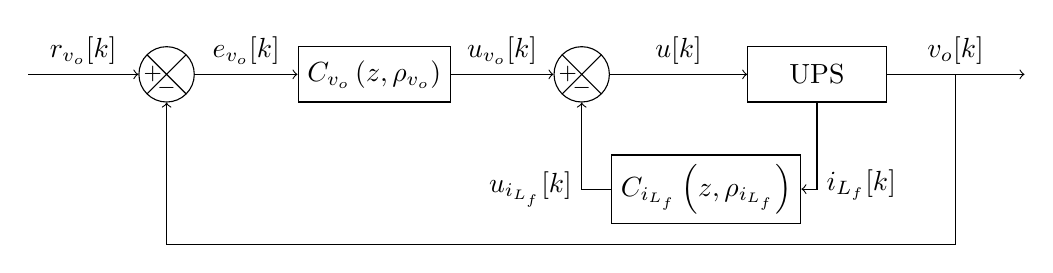
\begin{tikzpicture}[auto, node distance=7.5em]
        \node [input, name=input] {};
        \node [draw, circle, add={$-$}{$+$}{}{}, right of=input, node distance=5em] (sum1) {};
        \node [block, right of=sum1] (cvo) {$\myCzrho{\myvo}$};
        \node [draw, circle, add={$-$}{$+$}{}{}, right of=cvo] (sum2) {};
        \node [block, right of=sum2, node distance=8.5em] (gups) {UPS};
        \node [output, right of=gups, node distance=7.5em] (output) {};

        \draw [->] (input) -- node {$r_\myvo[k]$} (sum1);
        \draw [->] (sum1) -- node {$e_\myvo[k]$} (cvo);
        \draw [->] (cvo) -- node {$u_\myvo[k]$} (sum2);
        \draw [->] (sum2) -- node[name=u] {$u[k]$} (gups);
        \draw [->] (gups) -- node [name=y] {$\myvo[k]$} (output);

        \node [coordinate, below of=u, node distance=5em] (ubelow) {};
        \node [block, right of=ubelow, node distance=1em] (ci) {$\myCzrho{\myilf}$};

        \draw [->] (gups) |- node [pos=0.475] {$\myilf[k]$} (ci);
        \draw [->] (ci) -| node {$u_\myilf[k]$} (sum2);

        \node [coordinate, right of=gups, node distance=5em] (fo) {};
        \node [coordinate, below of=ci, node distance=2em] (fe) {};
        \draw [-] (fo) |- (fe);
        \draw [->] (fe) -| (sum1);
    \end{tikzpicture}
    }%
    \\\sourcecitation{do autor}
    \label{fig:UPS-control}
\end{figure}

%O sistema representado pela Figura \ref{fig:UPS-control} é equivalente àquele da Figura \ref{fig:cascadeloop1}.
O sistema representado pela Figura \ref{fig:UPS-control} é semelhante àquele da Figura \ref{fig:cascadeloop1}, com um controlador no laço de realimentação interno e outro sobre o erro de referência.
A tensão de saída $\myvo[k]$ corresponde ao sinal externo $y_e[k]$, enquanto a corrente no indutor $\myilf[k]$ condiz com o sinal interno $y_i[k]$.
Analogamente, o controlador de tensão $\myCzrho{\myvo}$ equivale ao controlador externo $\myCzrho{e}$, e o controlador de corrente $\myCzrho{\myilf}$ ao controlador interno $\myCzrho{i}$.
Assim, o projeto dos controladores por VRFT a partir de dados de um único ensaio, apresentada na Seção \ref{sec:VRFT_cascata}, pode ser aplicado para este sistema.
%As equivalências entre os controladores são transportadas para as definições do vetor de parâmetros $\rho$ e do vetor de regressão $\varphi(z)$.

%O controlador $\myCzrho{\myvo}$ é da classe PMR, a fim de proporcionar tanto seguimento de referência senoidal como atenuação de suas harmônicas.
A fim de proporcionar tanto seguimento de referência senoidal como atenuação de suas harmônicas, o controlador $\myCzrho{\myvo}$ é da classe PMR.
Este controlador é aplicado primeiramente considerando apenas a frequência fundamental, seguido pela inclusão de harmônicas ímpares até atingir a 9{\textordfeminine} ordem.
%Sob a carga não linear de teste, as harmônicas ímpares de menor ordem são as mais pronunciadas.
%Assim, este controlador será projetado para atuar sobre elas, notadamente, as harmônicas de ordem 3, 5, 7 e 9.
Considerando todas as possíveis frequências, a parametrização deste controlador é
% \begin{equation}
% \begin{gathered}
%     \myCzrho{\myvo} = \rho_\myvo \mycdot \myoC[\myvo]{z}
%     \,,
%     \\
%     \rho_\myvo =
%     \begin{bmatrix}
%         k_{PR} \\
%         k_{R_{1_{1}}} \\
%         k_{R_{1_{0}}} \\
%         k_{R_{3_{1}}} \\
%         k_{R_{3_{0}}} \\
%         \vdots \\
%         k_{R_{n_{1}}} \\
%         k_{R_{n_{0}}} \\
%     \end{bmatrix}^T
%     ,\;
%     \myoC[\myvo]{z} =
%     \begin{bmatrix}
%         1 \\
%         \frac{ z }{ z^2 - 2 \mycdot \cos \left( \Omega_1 \right) \mycdot z + 1 } \\
%         \frac{ 1 }{ z^2 - 2 \mycdot \cos \left( \Omega_1 \right) \mycdot z + 1 } \\
%         \frac{ z }{ z^2 - 2 \mycdot \cos \left( 3 \mycdot \Omega_1 \right) \mycdot z + 1 } \\
%         \frac{ 1 }{ z^2 - 2 \mycdot \cos \left( 3 \mycdot \Omega_1 \right) \mycdot z + 1 } \\
%         \vdots \\
%         \frac{ z }{ z^2 - 2 \mycdot \cos \left( n \mycdot \Omega_1 \right) \mycdot z + 1 } \\
%         \frac{ 1 }{ z^2 - 2 \mycdot \cos \left( n \mycdot \Omega_1 \right) \mycdot z + 1 } \\
%     \end{bmatrix}
%     \,,
% \end{gathered}
% \end{equation}
\begin{equation}
\begin{gathered}
    \myCzrho{\myvo} = \rho_\myvo \mycdot \myoC[\myvo]{z}
    \,,
    \\
    {\rho_\myvo}^T =
    \begin{bmatrix}
        k_{PR} \\
        k_{R_{1_{1}}} \\
        k_{R_{1_{0}}} \\
        k_{R_{3_{1}}} \\
        k_{R_{3_{0}}} \\
        k_{R_{5_{1}}} \\
        k_{R_{5_{0}}} \\
        k_{R_{7_{1}}} \\
        k_{R_{7_{0}}} \\
        k_{R_{9_{1}}} \\
        k_{R_{9_{0}}} \\
    \end{bmatrix}
    \,,\;
    \myoC[\myvo]{z} =
    \begin{bmatrix}
        1 \\
        \frac{ z }{ z^2 - 2 \mycdot \cos \left( \Omega_1 \right) \mycdot z + 1 } \\
        \frac{ 1 }{ z^2 - 2 \mycdot \cos \left( \Omega_1 \right) \mycdot z + 1 } \\
        \frac{ z }{ z^2 - 2 \mycdot \cos \left( \Omega_3 \right) \mycdot z + 1 } \\
        \frac{ 1 }{ z^2 - 2 \mycdot \cos \left( \Omega_3 \right) \mycdot z + 1 } \\
        \frac{ z }{ z^2 - 2 \mycdot \cos \left( \Omega_5 \right) \mycdot z + 1 } \\
        \frac{ 1 }{ z^2 - 2 \mycdot \cos \left( \Omega_5 \right) \mycdot z + 1 } \\
        \frac{ z }{ z^2 - 2 \mycdot \cos \left( \Omega_7 \right) \mycdot z + 1 } \\
        \frac{ 1 }{ z^2 - 2 \mycdot \cos \left( \Omega_7 \right) \mycdot z + 1 } \\
        \frac{ z }{ z^2 - 2 \mycdot \cos \left( \Omega_9 \right) \mycdot z + 1 } \\
        \frac{ 1 }{ z^2 - 2 \mycdot \cos \left( \Omega_9 \right) \mycdot z + 1 } \\
    \end{bmatrix}
    \,,
\end{gathered}
\end{equation}
em que $\Omega_i$ é a frequência discretizada da harmônica de ordem $i$.
Considerando uma frequência fundamental $f_1$ de $60 \text{ Hz}$ e um período de amostragem $T_s$ equivalente ao passo de simulação do Simulink, os valores das harmônicas de interesse são enunciados na Tabela \ref{tab:freq}, em consonância com a Equação \eqref{eq:ress_Omega}.
Novamente, destaca-se que o número de parâmetros a sintonizar é $2 \mycdot n + 1$, em que $n$ é o número de frequências consideradas.
%Os elementos referentes às harmônicas desconsideradas podem ser removidos dos vetores.

\begin{table}[h]
    \newcolumntype{C}[1]{>{\centering\arraybackslash}m{#1}}
    \centering
    \caption{Frequências de interesse.}
    \begin{tabular}{C{0.36\linewidth}|c|c|c|c|c}
        \textbf{Ordem} $\left( i \right)$                                                                & \textbf{1} & \textbf{3} & \textbf{5} & \textbf{7} & \textbf{9} \\\hline
        \textbf{Frequência} $\left( f_i \right)$ $\left[\text{Hz}\right]$                                & 60         & 180        &  300       & 420        &  540       \\\hline
        \textbf{Frequência Angular} $\left( \omega_i \right)$ $\left[\frac{\text{rad}}{\text{s}}\right]$ & 376,99     & 1130,97    & 1884,96    & 2638,94    & 3392,92    \\\hline
        \textbf{Frequência Discretizada} $\quad\left( \Omega_i \right)$ $\left[\text{rad}\right]$             & 0,01745    & 0,05236    & 0,08727    & 0,1222     & 0,1571     \\
    \end{tabular}
    \\\vspace{0.25cm}\sourcecitation{do autor}
    \label{tab:freq}
\end{table}

O controlador $\myCzrho{\myilf}$, por sua vez, é puramente proporcional.
Sua parametrização tem o seguinte formato:
\begin{equation}
\begin{gathered}
    \myCzrho{\myilf} = \rho_\myilf \mycdot \myoC[\myilf]{z}
    \,,
    \\
    %\rho_\myilf = \begin{bmatrix} K_P \end{bmatrix}
    \rho_\myilf = k_P
    \,,\;
    %\myoC[\myilf]{z} = \begin{bmatrix} 1 \end{bmatrix}
    \myoC[\myilf]{z} = 1
    \,.
\end{gathered}
\end{equation}

\section{Sintonia do Controlador por VRFT}

Além da definição da classe dos controladores, a aplicação do método VRFT envolve a realização de um ensaio para a coleta de dados do sistema, a determinação de um modelo de referência que especifica o comportamento desejado em malha fechada, e a especificação dos filtros.
Após essas etapas, a sintonia do controlador é realizada pela minimização do custo de referência virtual.

\subsection{Coleta de Dados}

A aplicação do método VRFT requer um ensaio sobre o sistema a ser controlado, o qual pode ser realizado em malha aberta ou fechada.
No caso da UPS, devem ser coletados os sinais de atuação, da tensão de saída e da corrente no indutor do filtro LC.

Neste ensaio, o sinal de atuação deve ser escolhido adequadamente.
Para obter bons resultados no projeto do controlador, é importante que o sistema seja excitado com um amplo espectro frequencial \cite{Bazanella2011}.

Em seus trabalhos \textcite{Corleta2015, Corleta2016, Bruna2020} realizam o ensaio para coleta de dados em malha aberta e com carga linear, com duração de um segundo.
O sinal aplicado sobre a UPS é uma soma de seis senoides com $10 \text{ V}$ ou $30 \text{ V}$ de amplitude e as seguintes frequências: $10 \text{ Hz}$, $60 \text{ Hz}$, $100 \text{ Hz}$, $150 \text{ Hz}$, $200 \text{ Hz}$ e $300 \text{ Hz}$.

Neste trabalho, são experimentadas diferentes configurações para a coleta de dados, variando inclusive o sinal aplicado.
Os ensaios são realizados com cargas linear e não linear máximas, e com a malha de controle aberta e fechada.

Para a malha aberta, os seguintes sinais são aplicados:
a soma de senoides supracitada;
a mesma soma acrescida de mais senoides, incluindo as harmônicas ímpares de $60 \text{ Hz}$ de ordem 3 a 9;
sequência binária pseudorrandômica --- Pseudorandom Binary Sequence (PRBS) --- com $30 \text{ V}$ de amplitude e banda de $30$ amostras, equivalente a aproximadamente $1,38 \text{ ms}$;
PRBS com $30 \text{ V}$ de amplitude e banda de $100$ amostras, aproximadamente $4,63 \text{ ms}$; e
PRBS com $30 \text{ V}$ de amplitude e banda de $200$ amostras, aproximadamente $9,26 \text{ ms}$.
O sinal PRBS é particularmente interessante por seu rico espectro frequencial.

Para a coleta de dados em malha fechada utilizou-se controladores obtidos a partir de um ensaio anterior em malha aberta.
Neste caso, define-se o sinal de referência, e o sinal de atuação é determinado pelos controladores.
Experimentou-se aplicar, somados à referência senoidal de frequência fundamental, os sinais PRBS supracitados.

Os melhores resultados --- em termos de iterações para a convergência dos parâmetros e desempenho em malha fechada --- são obtidos com dados coletados do ensaio em malha aberta com carga linear máxima e aplicação do PRBS com banda de $100$ amostras.
Os sinais coletados nesse ensaio são exibidos na Figura \ref{fig:prbs100}, limitados aos primeiros $500 \text{ ms}$ para melhor visualização.
As sintonias realizadas no decorrer deste trabalho utilizam esses dados.

%Embora o comportamento crítico ocorra com a carga não linear, \textcite{?} já mostrou que métodos baseados em dados coletados com a carga linear podem oferecer controladores com bom desempenho também para a carga não linear.

\begin{figure}[h]
    \centering
    \caption{Ensaio em malha aberta com 100\% da carga linear e aplicação de PRBS com $30 \text{ V}$ de amplitude e banda de $100$ amostras.}
    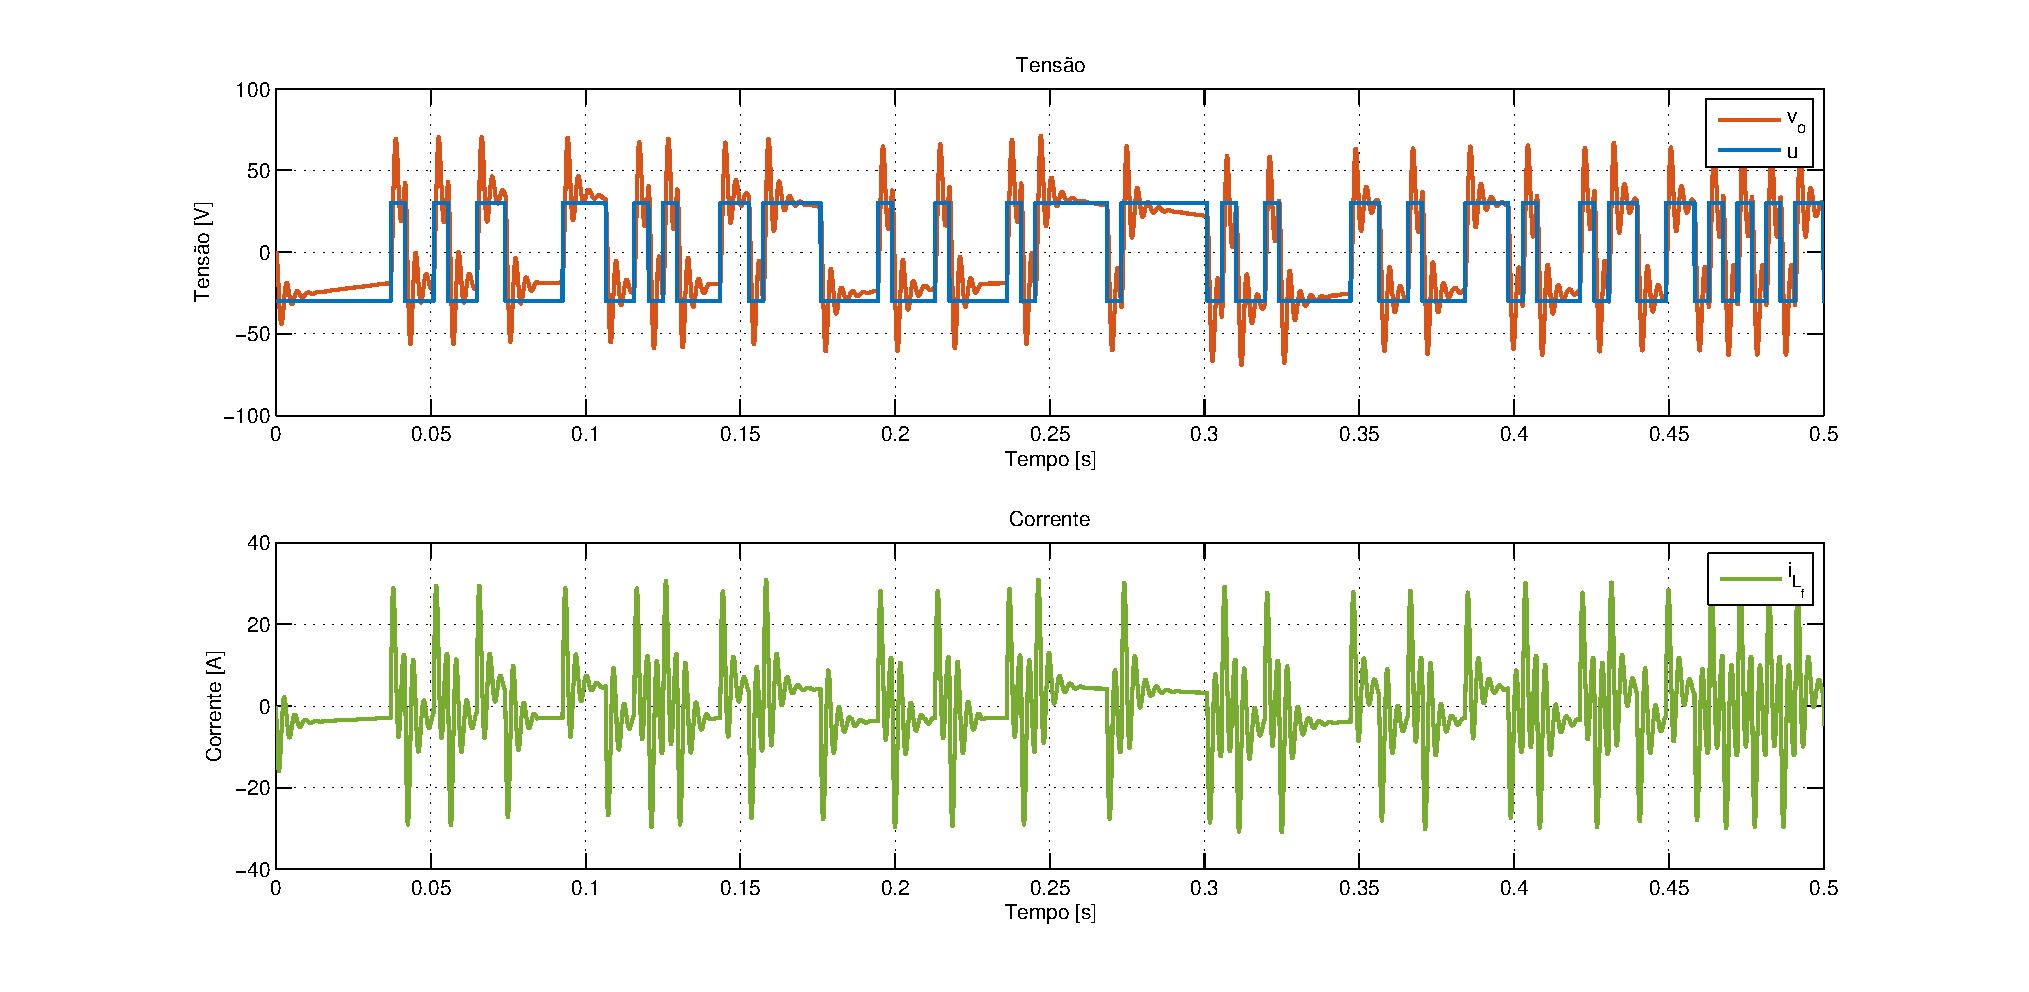
\includegraphics[trim={80 20 80 18}, clip, width=\linewidth]{fig/prbs100.eps}
    \\\sourcecitation{do autor}
    \label{fig:prbs100}
\end{figure}

\subsection{Modelo de Referência}

O modelo de referência é uma função de transferência que especifica o comportamento desejado para o sistema em malha fechada.
A escolha adequada desta função é essencial para o sucesso do método VRFT.
\textcite{Bazanella2011} enunciam diretrizes para essa escolha, algumas das quais são citadas a seguir.
Embora o completo conhecimento do processo a ser controlado seja dispensável, algumas informações são úteis para a composição do modelo de referência.

O comportamento dinâmico do modelo de referência deve ser próximo ao que é possível de atingir com a classe de controlador especificada.
Caso contrário, a sintonia obtida pode resultar em uma resposta completamente diferente.
Um comportamento excessivamente distante seria, por exemplo, um tempo de acomodação da resposta muito menor que o praticável.

Para que o controlador seja causal, o grau relativo do modelo desejado não pode ser menor que o grau relativo do processo.
Em trabalhos que modelam o estágio de saída da UPS, como o de \textcite{Pereira2014}, verifica-se que seu grau relativo é $2$.

\newpage
No entanto, a presença de um bloco de memória nos laços de realimentação, efetivamente atrasando o sinal medido em uma amostra, aparece na função de transferência em malha fechada como um zero adicional, posicionado na origem do plano $z$.
Além de ser interessante replicar esse zero no modelo de referência, ele permite que o grau relativo dessa função seja menor que o grau relativo do processo em uma unidade.
Assim, o grau relativo $1$ torna-se suficiente.

No caso do seguimento de referências senoidais, é imprescindível que o modelo de referência apresente, para a frequência em questão, ganho unitário e fase nula.
Caso contrário, o sinal de saída seria amplificado ou atenuado e deslocado em fase com relação ao sinal de referência.
Essa condição é matematicamente expressa por
\begin{equation}
\begin{aligned}
    \left| \left[ T_d(z) \right]_{z = e^{\pm j \mycdot \Omega_1 }} \right| = 1
    \,,\;
    &&
    \phase{\left[ T_d(z) \right]_{z = e^{\pm j \mycdot \Omega_1 }}} = 0
    \,.
\end{aligned}
\label{eq:cond_sen}
\end{equation}

\textcite{Corleta2015, Corleta2016, Bruna2020} utilizam um modelo de referência com um zero na origem, dois zeros reais em uma mesma posição e quatro polos também reais em uma mesma posição.
Os polos são escolhidos para fornecer um tempo de resposta suficientemente rápido, e os zeros são então calculados, a partir de uma abordagem geométrica, a fim de satisfazer a Equação \eqref{eq:cond_sen}.
Observe que o grau relativo desta função de transferência é $1$.

Inicialmente, este trabalho aplicou esta mesma abordagem para obter, com sucesso, um controlador considerando apenas a frequência fundamental.
Ao estender este controlador para a terceira harmônica, porém, verifica-se que a sintonia por VRFT tende a posicionar seus zeros sobre os polos dessa harmônica, efetivamente cancelando-os.
Isso ocorre justamente porque o modelo de referência empregado não especifica qualquer comportamento para essa frequência.

Na verdade, o modelo de referência especifica apenas a dinâmica do seguimento de referência.
Não é possível definir, diretamente, um comportamento desejado para a rejeição de perturbações.

A primeira abordagem para contornar este problema envolve incluir, na minimização do custo de referência virtual, restrições sobre os valores dos parâmetros do controlador.
Sendo os polos das harmônicas situados sobre o círculo unitário, uma limitação sobre o módulo dos zeros garantiria o não cancelamento, além de fornecer uma maneira de interferir em suas posições e, assim, também no comportamento dinâmico.
Observe, porém, que a minimização ocorre em função de um vetor de parâmetros, os quais, através de um polinômio, definem os zeros.
À medida que mais harmônicas são adicionadas, este polinômio passa a ter grau elevado, e a solução torna-se impraticável.
%Outras maneiras de estabelecer restrições foram cogitadas, mas nenhuma deles foi bem sucedida.

A segunda e derradeira abordagem é incluir, no modelo de referência, as condições para seguimento também de senoides com as frequências harmônicas, isto é, ganho unitário e fase nula.
Assim, os respectivos polos no controlador não podem ser cancelados, e a rejeição de perturbações com essas frequências é garantida indiretamente.

A função de transferência do modelo de referência é então construída para cumprir tais condições.
A fim de satisfazer o ganho unitário e fase nula em cada frequência de interesse, seu numerador deve apresentar um polinômio cujo número de parâmetros livres seja o dobro do número de frequências.
Além disso, um zero na origem é incluído para modelar o atraso de uma amostra na medição dos sinais.
Assim como em \textcite{Corleta2015, Bruna2020}, os polos são colocados todos em uma mesma posição, e a quantidade é determinada para que o grau relativo seja unitário.
A função de transferência resultante tem o seguinte formato:
\begin{equation} \label{eq:mr}
    T_d(z) = \dfrac{ z \mycdot \sum_{i = 0}^{n} k_i \mycdot z^i  }{ \left( z - p \right)^{n + 2} }
    \,,\;
    n = \{1, 3, 5, 7, 9\}
    \,.
\end{equation}
O valor dos polos $p$ está relacionado com o tempo de resposta do sistema.
Diferentes valores de $p$ são avaliados, conforme será descrito posteriormente.
Os coeficientes do polinômio do numerador, $k_i$ são determinados pela solução de um sistema de equações lineares:
cada frequência de interesse --- positiva e negativa --- é aplicada em $T_d(z)$, a qual é igualada a unidade, fornecendo uma equação.

Cabe citar ainda que, com este modelo de referência, o controlador ideal certamente não pertence à classe definida pelo controlador PMR na malha de tensão e P na de corrente.
Isto, no entanto, não caracteriza um problema para a aplicação do VRFT.

\subsection{Filtros}

O filtro ponderador $L(z)$ aproxima o custo de referência virtual $J_{vr}(\rho)$ ao custo do modelo de referência $J_{mr}(\rho)$.
Na topologia em cascata aplicada, este filtro depende da sensibilidade do laço de realimentação interna $S_i(z, \rho_i)$, o qual por sua vez é função do próprio controlador interno $\myCzrho{\myilf}$, a ser determinado, e do processo interno $\myG[i]{z}$, o qual é desconhecido.
Assim, este filtro deve ser estimado.

Neste trabalho aplica-se a metodologia desenvolvida por \textcite{Chrystian2020}, em que $S_i(z, \rho_i)$ é inicialmente arbitrado como um ganho unitário e é reestimado iterativamente.
Para essa estimativa, aplica-se a modelagem autorregressiva com entrada externa --- \textit{Autoregressive with Extra Input} (ARX) --- para obter uma função de transferência com dois polos e dois zeros.
Essa quantidade de polos e zeros baseia-se em trabalhos que realizam a modelagem da UPS, como o de \textcite{Pereira2014}.

O critério de convergência é arbitrado como a maior diferença relativa entre os parâmetros do vetor $\rho$ calculados na iteração atual e na anterior.
A tolerância relativa empregada é de $10^{-9}$.
Com esse valor, a convergência geralmente ocorre em até uma dezena de iterações.

\chapter{Resultados}\label{sec:resultados}

Esta seção discute os resultados obtidos.
O projeto inicialmente considera apenas a frequência fundamental para a obtenção de um controlador de tensão da classe PR, junto do controlador de corrente.
Gradativamente são incorporadas, em um controlador de tensão PMR, as harmônicas ímpares até a 9{\textordfeminine} ordem.
Para cada caso, diferentes posições de polos no modelo de referência são avaliadas.

Os resultados a seguir utilizam como exemplo o projeto considerando a frequência fundamental e a 3{\textordfeminine}, 5{\textordfeminine} e 7{\textordfeminine} harmônicas.
%O controlador obtido a partido deste projeto apresentou os melhores resultados.
Os demais casos são tratadas de forma similar, estando integralmente expostos nos apêndices \ref{app:varia_polo} e \ref{app:respostas}.

\section{Posicionamento dos Polos do Modelo de Referência}

O modelo de referência proposto, enunciado pela Equação \eqref{eq:mr}, permite escolher a posição de seu conjunto de polos.
Essa função de transferência estipula o comportamento desejado para o sistema em malha-fechada.
Naturalmente, para que o sistema seja estável, os polos devem estar no interior no círculo unitário.
Além disso, a posição está associada, diretamente, com o tempo de resposta e amortecimento e, indiretamente, com o esforço de controle exigido:
quanto mais próximos do círculo unitário, mais lenta é a resposta do sistema;
quanto maior o ângulo de fase, menor é o amortecimento;
respostas mais rápidas ou menos amortecidas tendem a exigir um maior esforço de controle.

Neste trabalho, opta-se por posicionar os polos sobre o eixo real positivo.
Além disso, como o período de amostragem é significativamente menor que a dinâmica do sistema, estes polos podem ser posicionados próximos ao círculo unitário e ainda assim fornecer uma resposta suficientemente rápida, como será mostrado.
Ambas as decisões procuram evitar a saturação do esforço de controle.
Destaca-se, ainda, que a precisão numérica dos valores da função de transferência --- sejam polos, zeros ou coeficientes --- exerce grande influência sobre os resultados, em especial quando a ordem é elevada.

A seleção dos polos parte de um procedimento analítico.
Primeiramente é traçado, para diferentes posições, o mapa de polos e zeros do modelo de referência.
Cabe citar que o conjunto de posições parte de uma estimativa inicial, sendo refinado pela repetição deste processo.
Posições que resultam em sistemas com fase não mínima --- isto é, com zeros fora do círculo unitário --- são descartadas.
A Figura \ref{fig:pz_M_7} mostra esse mapa para o projeto exemplo.
Note que, em todos os casos, há um zero fixo na origem.

\begin{figure}[h]
    \centering
    \caption{Efeito da variação dos polos do modelo de referência sobre seu mapa de polos e zeros considerando a frequência fundamental e a 3{\textordfeminine}, 5{\textordfeminine} e 7{\textordfeminine} harmônicas.}
    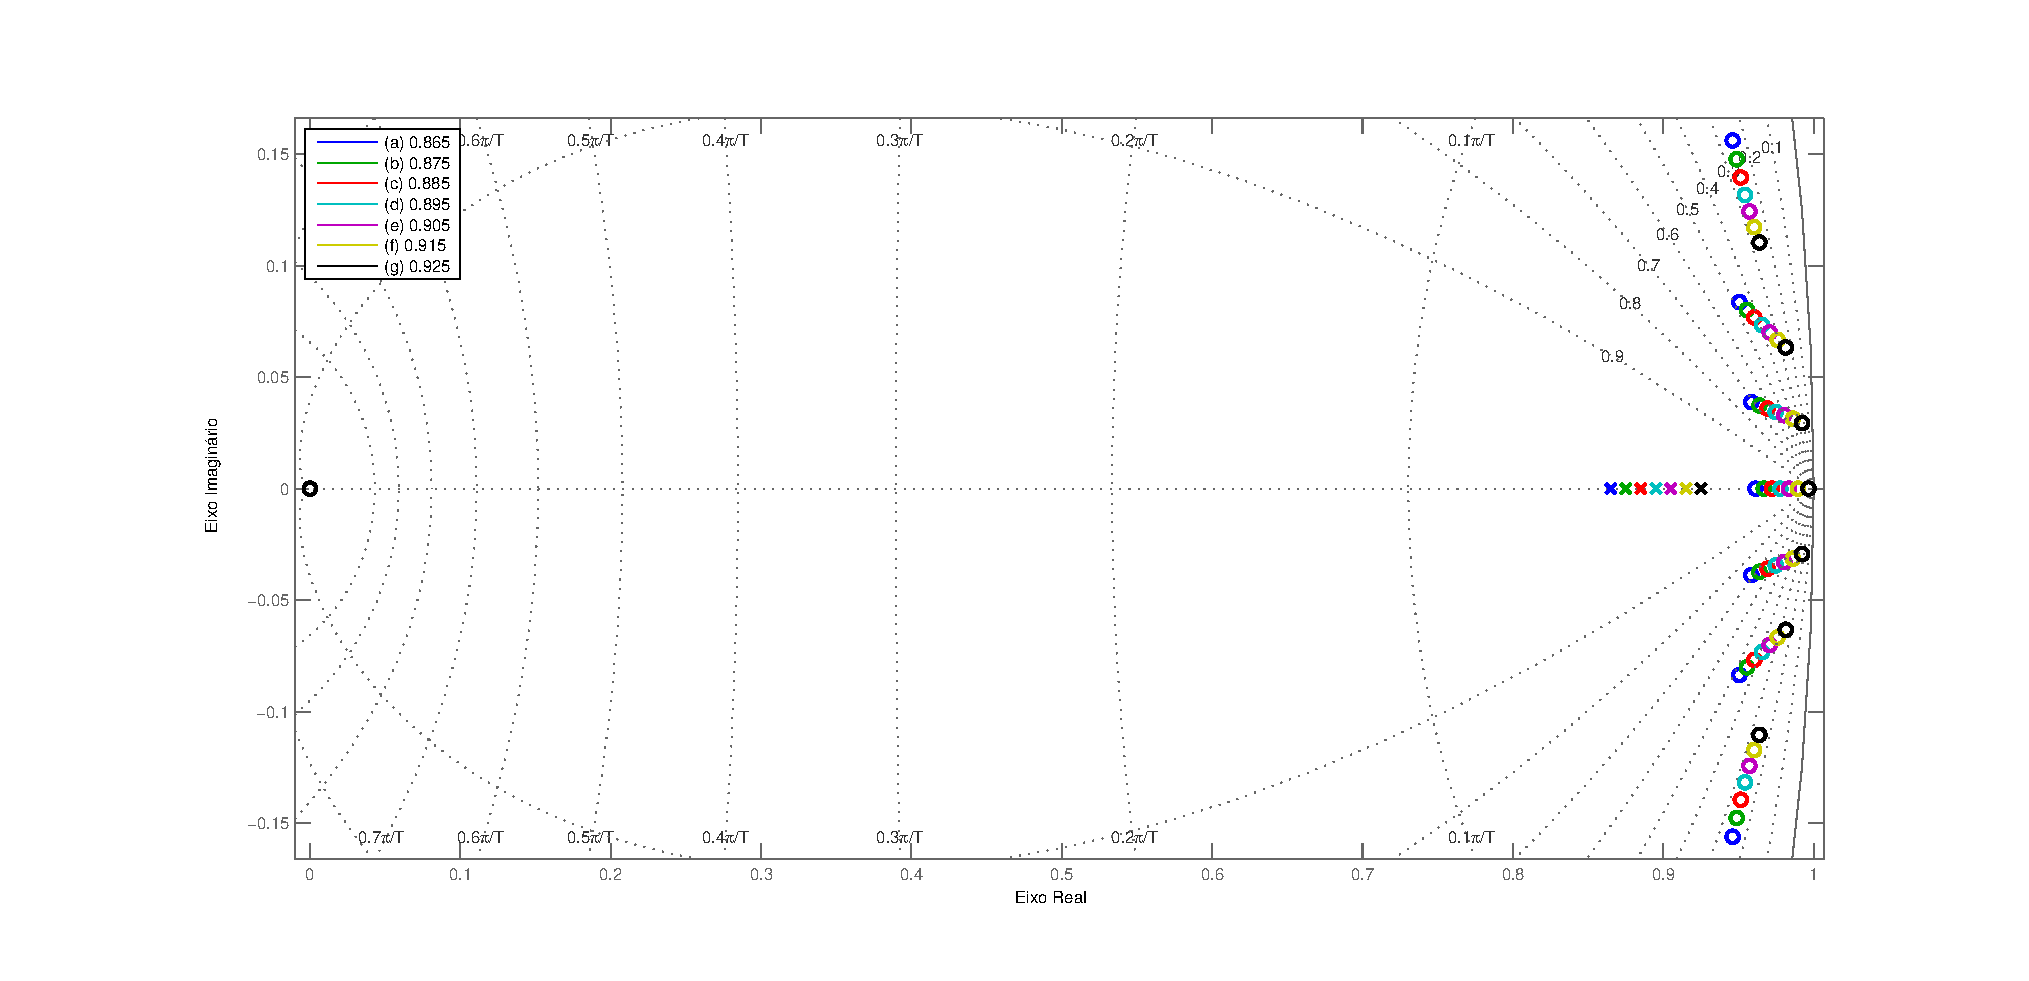
\includegraphics[trim={80 25 80 43}, clip, width=0.78\linewidth]{fig/pz_M_7.eps}
    \\\sourcecitation{do autor}
    \label{fig:pz_M_7}
\end{figure}

%Em seguida, para o conjunto de posições que resulta em um sistema de fase mínima, o diagrama de Bode é traçado.
Em seguida, o diagrama de Bode é traçado.
%Pelo diagrama de Bode, mostrado na Figura \ref{fig:bode_M_7} para o projeto exemplo, é possível verificar eventuais amplificações que podem ocorrer em certas frequências, bem como confirmar a fase mínima.
Pelo diagrama, mostrado na Figura \ref{fig:bode_M_7} para o projeto exemplo, é possível confirmar a fase mínima.
Este gráfico permite ainda visualizar as condições de módulo unitário --- no caso, $0 \text{ dB}$ --- e fase nula impostas sobre as frequências de interesse.

\begin{figure}[h]
    \centering
    \caption{Efeito da variação dos polos do modelo de referência sobre seu diagrama de Bode considerando a frequência fundamental e a 3{\textordfeminine}, 5{\textordfeminine} e 7{\textordfeminine} harmônicas.}
    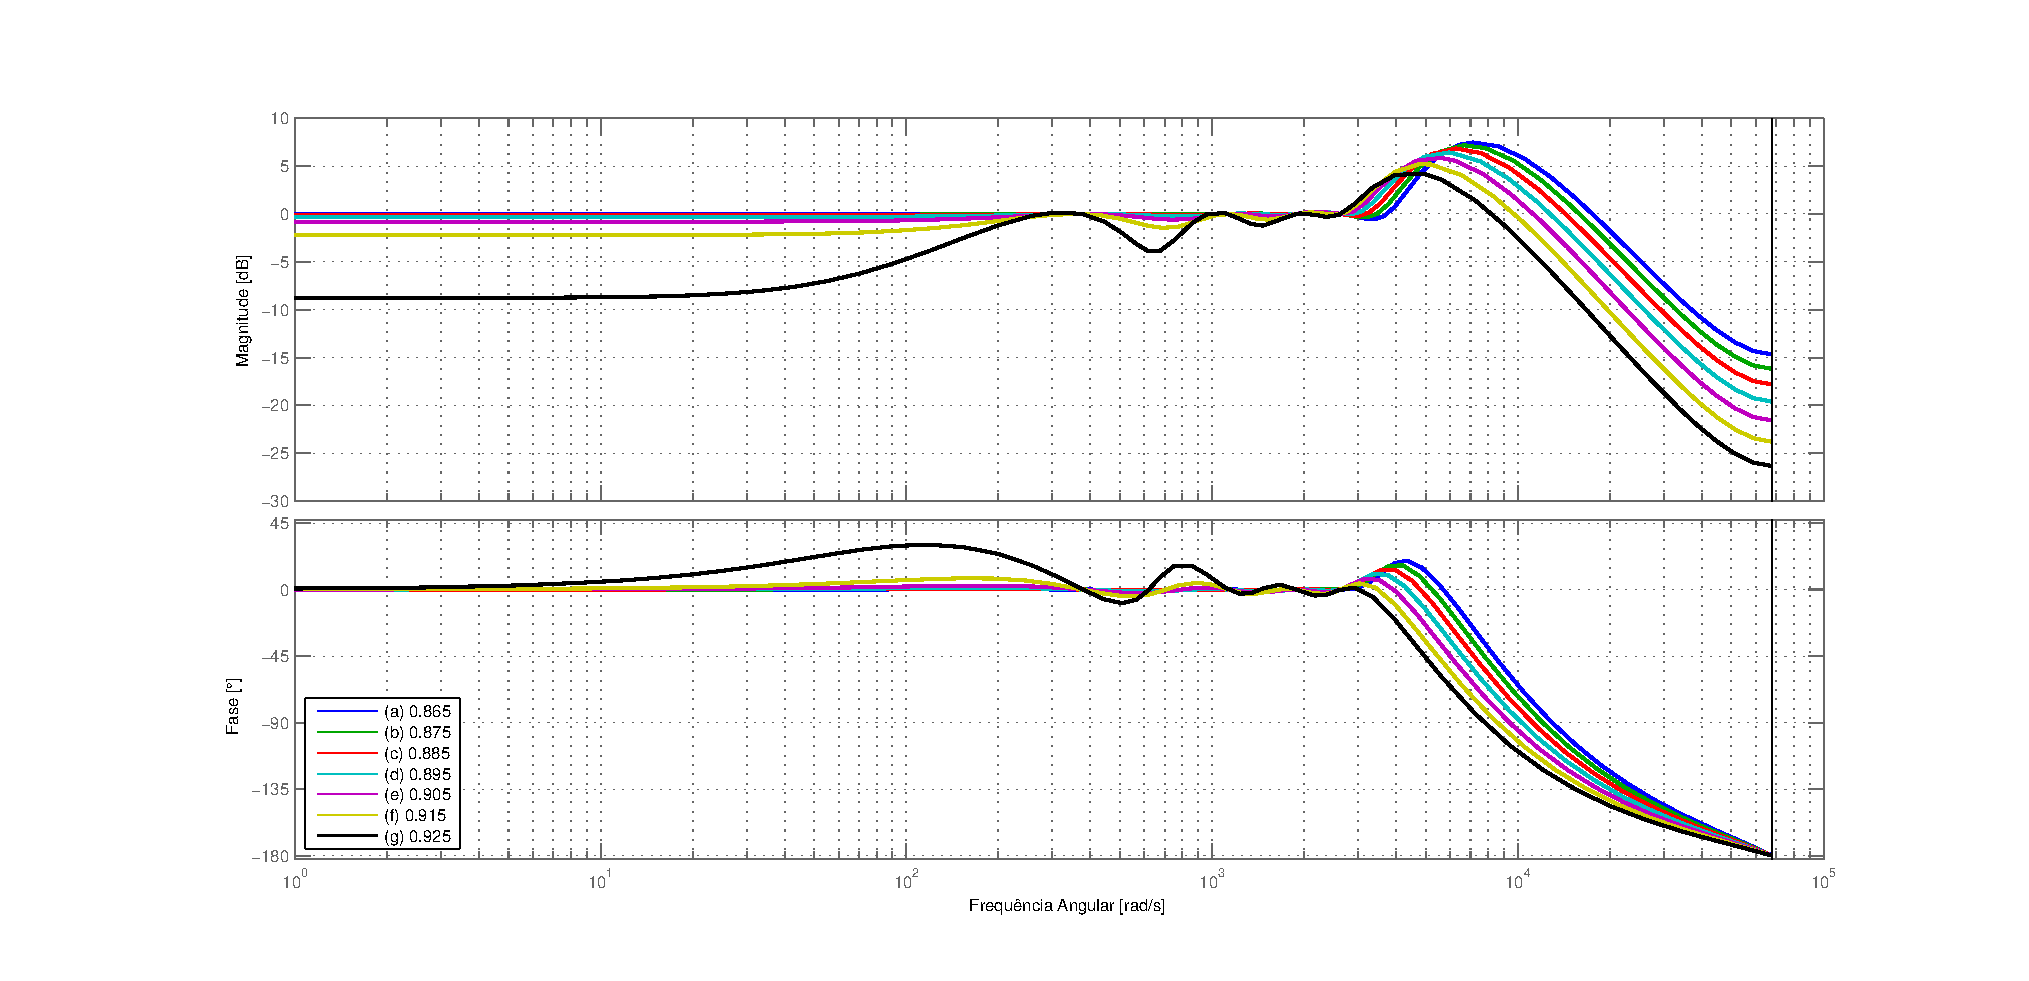
\includegraphics[trim={80 24.5 80 43}, clip, width=0.78\linewidth]{fig/bode_M_7.eps}
    \\\sourcecitation{do autor}
    \label{fig:bode_M_7}
\end{figure}

\newpage

Também é realizada a análise sobre a resposta à entrada senoidal.
O resultado para o projeto exemplo é exibido na Figura \ref{fig:sinsim_M_7}.
Através deste gráfico é possível visualizar o tempo de resposta ao seguimento da referência.
Na posterior seleção do controlador, procura-se escolher um que provenha de um modelo cujo tempo de acomodação ocorra próximo a metade do primeiro ciclo da senoide.
Esse critério provém de resultados observacionais, fornecendo uma boa relação entre tempo de resposta e máximo esforço de controle.

\begin{figure}[h]
    \centering
    \caption{Efeito da variação dos polos do modelo de referência sobre sua resposta a senoide considerando a frequência fundamental e a 3{\textordfeminine}, 5{\textordfeminine} e 7{\textordfeminine} harmônicas.}
    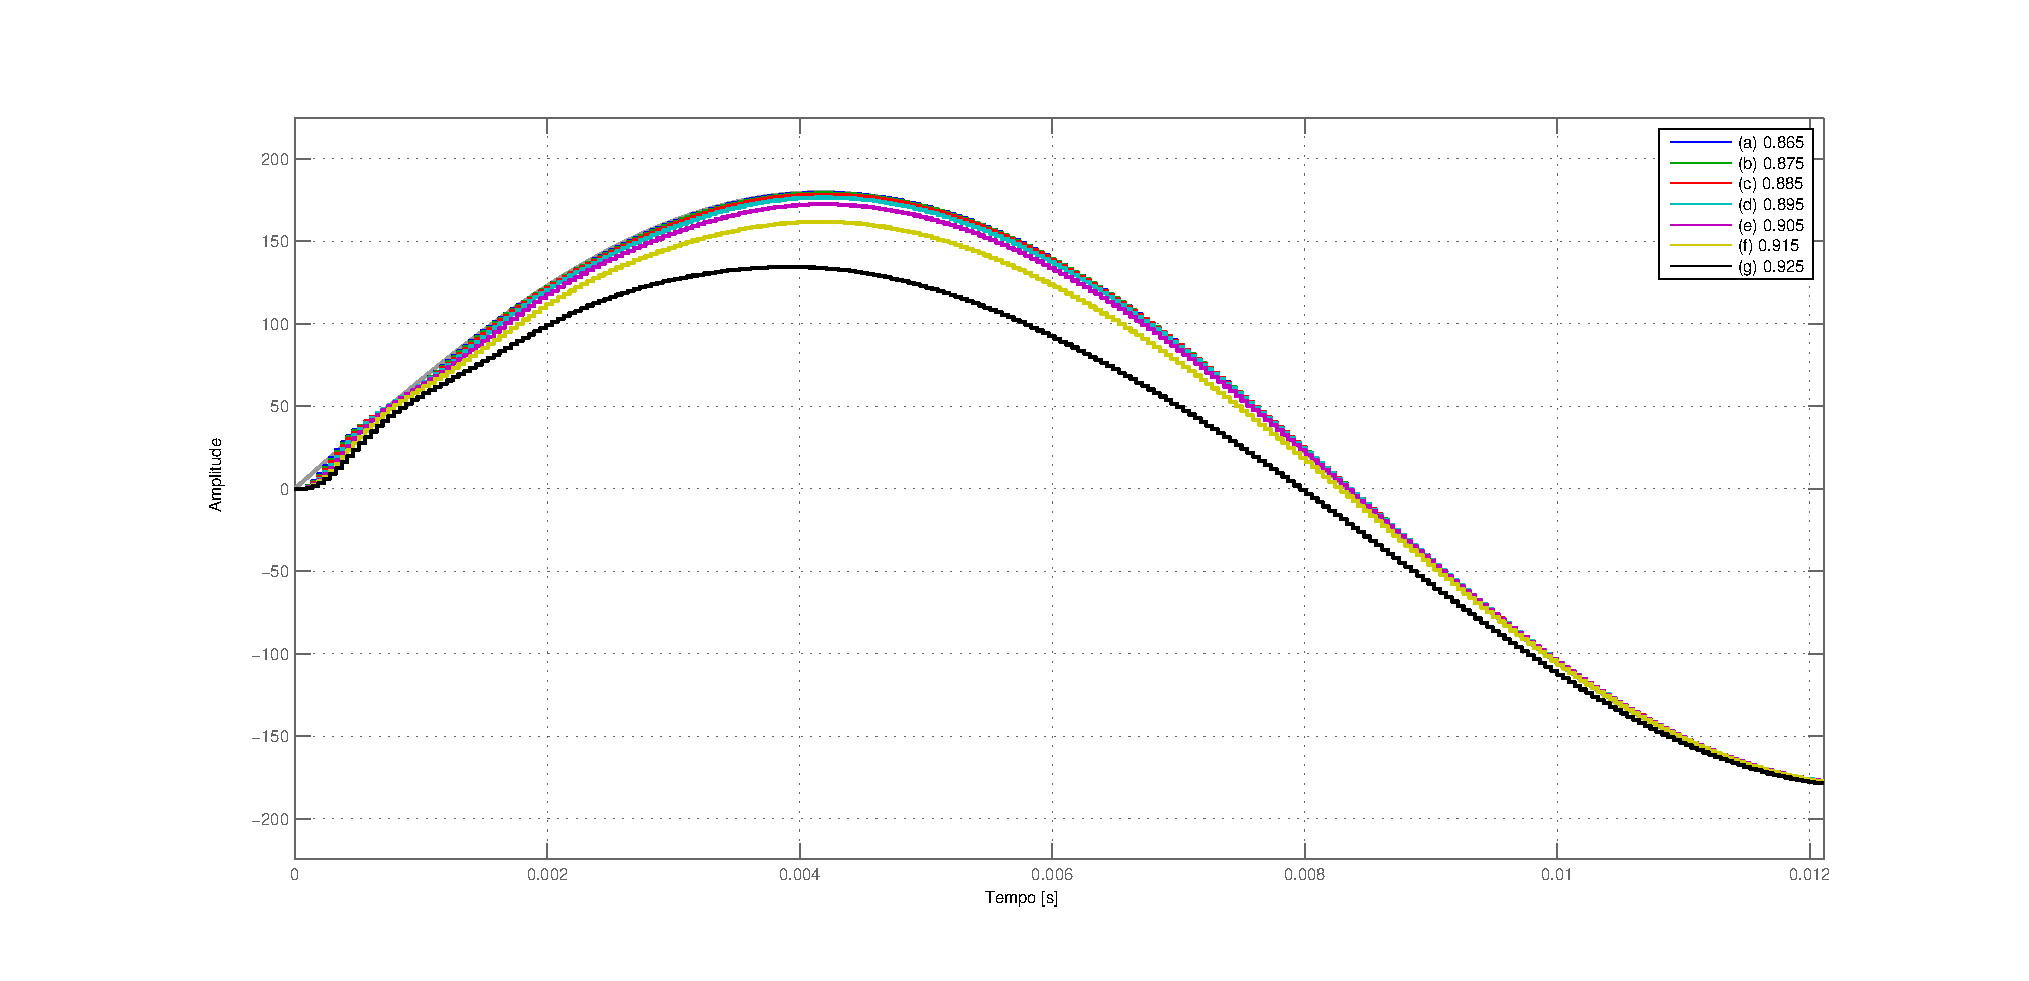
\includegraphics[trim={80 25 80 43}, clip, width=0.78\linewidth]{fig/sinsim_M_7.eps}
    \\\sourcecitation{do autor}
    \label{fig:sinsim_M_7}
\end{figure}

Finalmente, são obtidos os respectivos parâmetros dos controladores, e o mapa de polos e zeros do controlador de tensão é construído.
Controladores com zeros no exterior do círculo unitário não são interessantes, sendo descartados.
Este mapa, correspondente ao projeto exemplo, é apresentado pela Figura \ref{fig:pz_C1_7}.
Ali observa-se um comportamento característico de cada zero do controlador de acordo com as posição dos polos do modelo de referência.
Reitera-se que todos os controladores apresentam os polos nas mesmas posições, as quais são previamente especificadas.

\begin{figure}[h]
    \centering
    \caption{Efeito da variação dos polos do modelo de referência sobre o mapa de polos e zeros do controlador de tensão considerando a frequência fundamental e a 3{\textordfeminine}, 5{\textordfeminine} e 7{\textordfeminine} harmônicas.}
    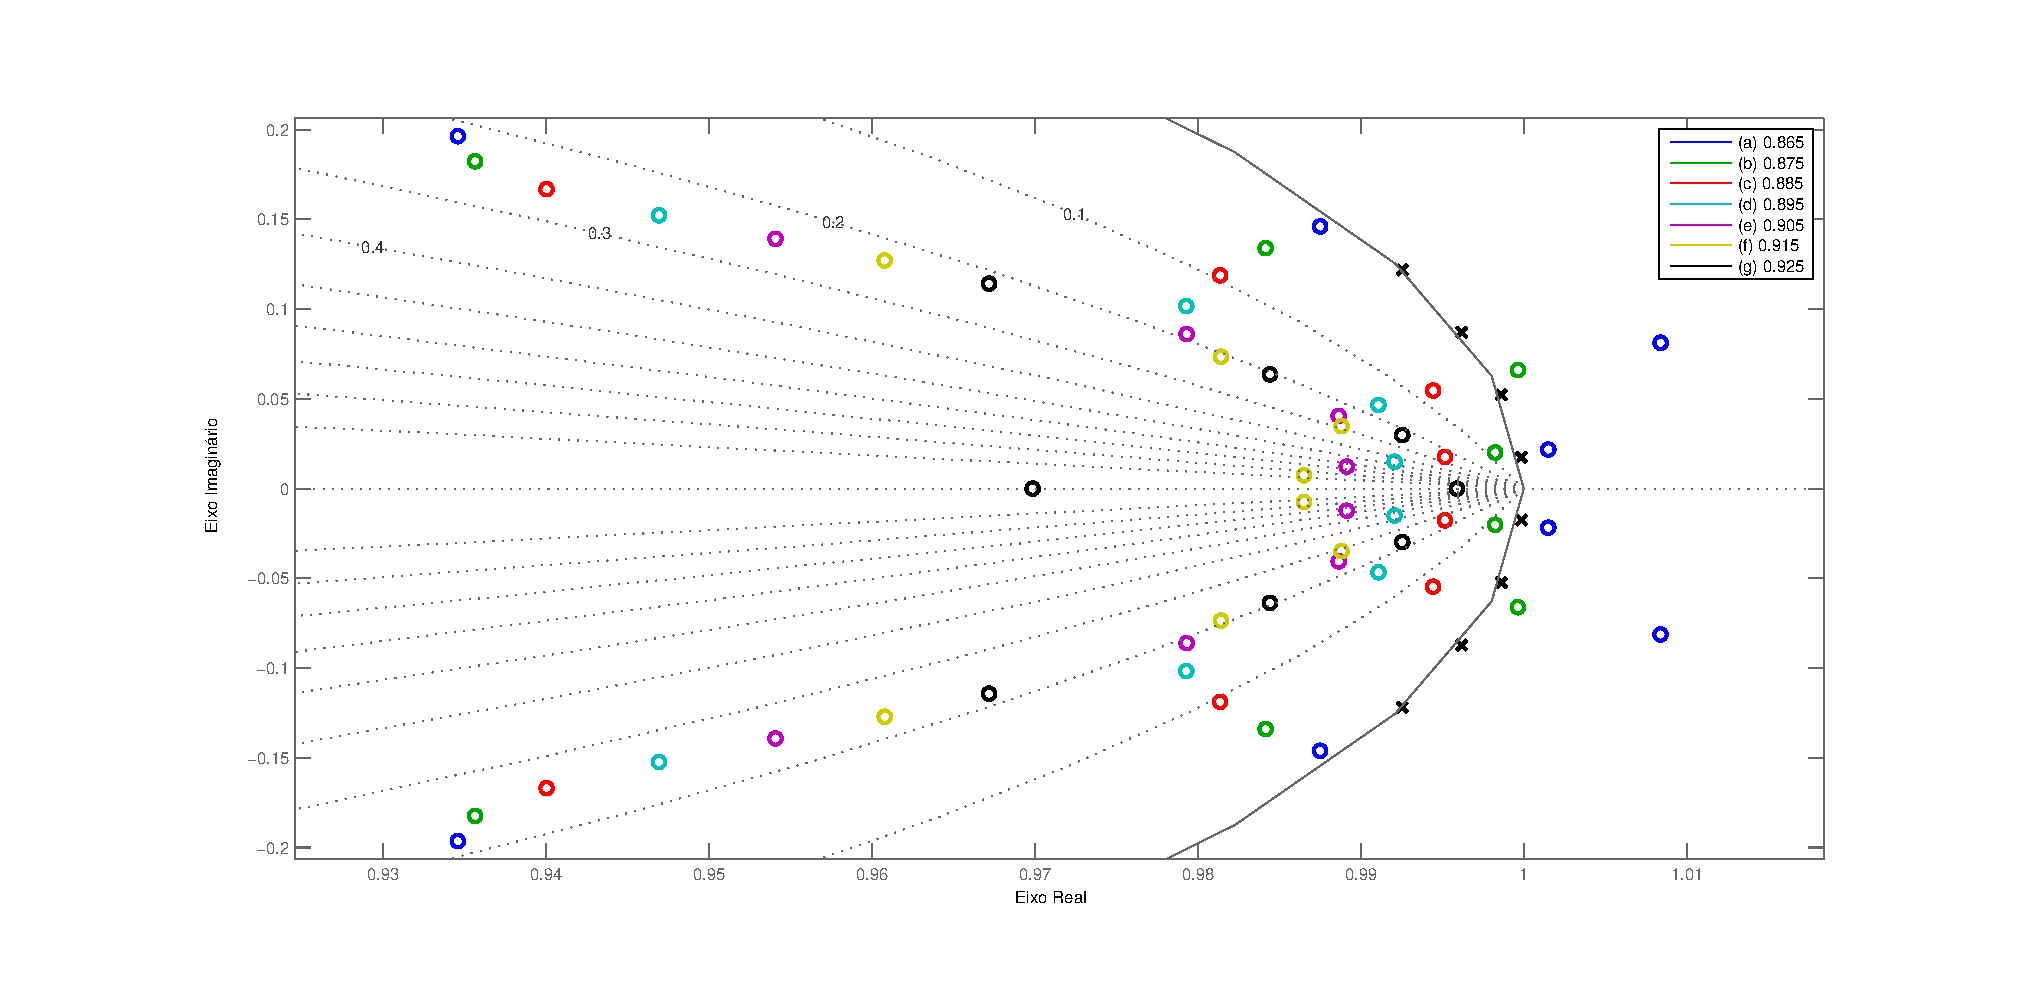
\includegraphics[trim={80 25 80 43}, clip, width=0.78\linewidth]{fig/pz_C1_7.eps}
    \\\sourcecitation{do autor}
    \label{fig:pz_C1_7}
\end{figure}

O controlador é então selecionado dentre aqueles obtidos neste processo.
Após sua aplicação no sistema em malha fechada, o desempenho é analisado.
Caso não seja satisfatório, uma nova posição é testada, ou o procedimento é repetido para uma nova faixa de posições de polos do modelo de referência.

Através desse procedimento, é selecionado no projeto exemplo o modelo de referência com polos em $0,915$, rotulado como \texttt{(f)}.
Sua função de transferência é
\begin{equation}
    \resizebox{.97\textwidth}{!}{$%
    T_d(z) = \dfrac{  0,189  z \left(z-0,9895\right) \left(z^2 - 1,972 \mycdot z + 0,9734\right) \left(z^2 - 1,952 \mycdot z + 0,957\right) \left(z^2 - 1,921 \mycdot z + 0,9361\right) }
                   { \left( z - 0,915 \right)^9 }
    \,.
    $}%
\end{equation}

\section{Controladores}

Os controladores selecionados são especificados na Tabela \ref{tab:rhos}, através de seus parâmetros.
Além de verificar a posição dos zeros, tanto do modelo como do controlador de tensão, no interior do círculo unitário, a seleção considera um tempo de acomodação adequado na resposta à senoide, próximo à metade do primeiro ciclo.
%Para o projeto exemplo, em que a ordem da maior harmônica é 7, é escolhido o controlador provindo do modelo de referência com polos em $0,915$, rotulado como \texttt{(f)}.

\begin{table}[h]
    \newcolumntype{C}[1]{>{\centering\arraybackslash}m{#1}}
    \centering
    \caption{Parâmetros dos controladores obtidos.}
    \resizebox{.97\textwidth}{!}{%
    \begin{tabular}{C{0.35\linewidth}|c|c|c|c|c}
                                                 & \multicolumn{5}{c}{\textbf{Ordem da Maior Harmônica}}            \\
                                                 & \textbf{1}  & \textbf{3} & \textbf{5} & \textbf{7} & \textbf{9}  \\\hline
        Posição dos polos de $T_d(z)$            & $0,955$     & $0,94$     & $0,932$    & $0,915$    & $0,91$      \\\hline
        Iterações para convergência              & $4$         & $4$        & $5$        & $5$        & $47$        \\\hline
        Ajuste da estimativa de $S_i(z, \rho_i)$ & $92,95\%$   & $91,25\%$  & $90,28\%$  & $90,0\%$   & $90,35\%$   \\\hline
        $k_{PR}$                                 & $ 0,84455 $ & $ 4,6444 $ & $11,43   $ & $26,152  $ & $37,23    $ \\\hline
        $k_{R_{1_{1}}}$                          & $ 0,079013$ & $ 0,16945$ & $ 0,14149$ & $ 0,2273 $ & $ 0,084488$ \\%\hline
        $k_{R_{1_{0}}}$                          & $-0,078551$ & $-0,16978$ & $-0,14296$ & $-0,23029$ & $-0,086172$ \\\hline
        $k_{R_{3_{1}}}$                          & -           & $ 0,22365$ & $ 0,33714$ & $ 0,38952$ & $-0,10678 $ \\%\hline
        $k_{R_{3_{0}}}$                          & -           & $-0,21851$ & $-0,35367$ & $-0,43255$ & $ 0,086904$ \\\hline
        $k_{R_{5_{1}}}$                          & -           & -          & $ 0,66347$ & $ 1,8485 $ & $-0,13383 $ \\%\hline
        $k_{R_{5_{0}}}$                          & -           & -          & $-0,63604$ & $-1,936  $ & $-0,027243$ \\\hline
        $k_{R_{7_{1}}}$                          & -           & -          & -          & $ 1,1798 $ & $ 3,9995  $ \\%\hline
        $k_{R_{7_{0}}}$                          & -           & -          & -          & $-0,88456$ & $-4,6255  $ \\\hline
        $k_{R_{9_{1}}}$                          & -           & -          & -          & -          & $ 1,6778  $ \\%\hline
        $k_{R_{9_{0}}}$                          & -           & -          & -          & -          & $-0,65819 $ \\\hline
        $k_P$                                    & $ 3,9445  $ & $ 6,0561 $ & $ 7,9946 $ & $ 8,753  $ & $ 7,8107  $ \\
    \end{tabular}
    }%
    \\\vspace{0.25cm}\sourcecitation{do autor}
    \label{tab:rhos}
\end{table}

\newpage
A Tabela \ref{tab:rhos} inclui ainda o número de iterações para a convergência dos parâmetros e o ajuste final obtido para a estimativa da sensibilidade interna $S_i(z, \rho_i)$, conforme fornecido pela função ARX do MATLAB.
Observe que, mesmo utilizando um ganho unitário como estimativa inicial, a convergência é rápida, com exceção do caso que considera a 9{\textordfeminine} harmônica.
Ademais, a estimativa final apresenta um ajuste superior a $90\%$ em todos os casos.

% Destaca-se aqui que, no caso em que a 9{\textordfeminine} harmônica é considerada, não foram obtidos controladores capazes de manter o sistema em malha fechada estável, mesmo após ampla experimentação com diferentes posições dos polos do modelo de referência, e até mesmo com modelos alternativos.
% Neste caso específico, os sistemas seguem a referência senoidal apenas em seus primeiros ciclos, logo tendendo a instabilidade.

\section{Desempenho em Malha Fechada}

% Por apresentar um comportamento em malha fechada instável, não é avaliado o desempenho do controlador cuja ordem da maior harmônica é 9.
% Os demais controladores selecionados proporcionam, em malha fechada, o seguimento da referência senoidal, tanto sob carga linear como não linear.

Para avaliar o desempenho o seguinte teste, com duração total de um segundo, é aplicado sobre a UPS simulada em malha fechada, com carga linear e não linear:
o sistema parte do repouso com carga mínima;
após $0,3375 \text{ s}$, no pico do sinal de referência, ocorre o degrau aditivo de carga, para o valor máximo;
no instante de tempo $0,6708 \text{ s}$, também no pico do sinal de referência, ocorre o degrau subtrativo de carga, retornando para o valor mínimo.
O tempo decorrido entre cada evento é suficiente para que a resposta atinja o regime permanente.
Este ensaio é apresentado para o projeto exemplo na Figura \ref{fig:closed_7_full}.

\begin{figure}[h]
    \centering
    \caption{Ensaio utilizando o controlador para a frequência fundamental e a 3{\textordfeminine}, 5{\textordfeminine} e 7{\textordfeminine} harmônicas.}
    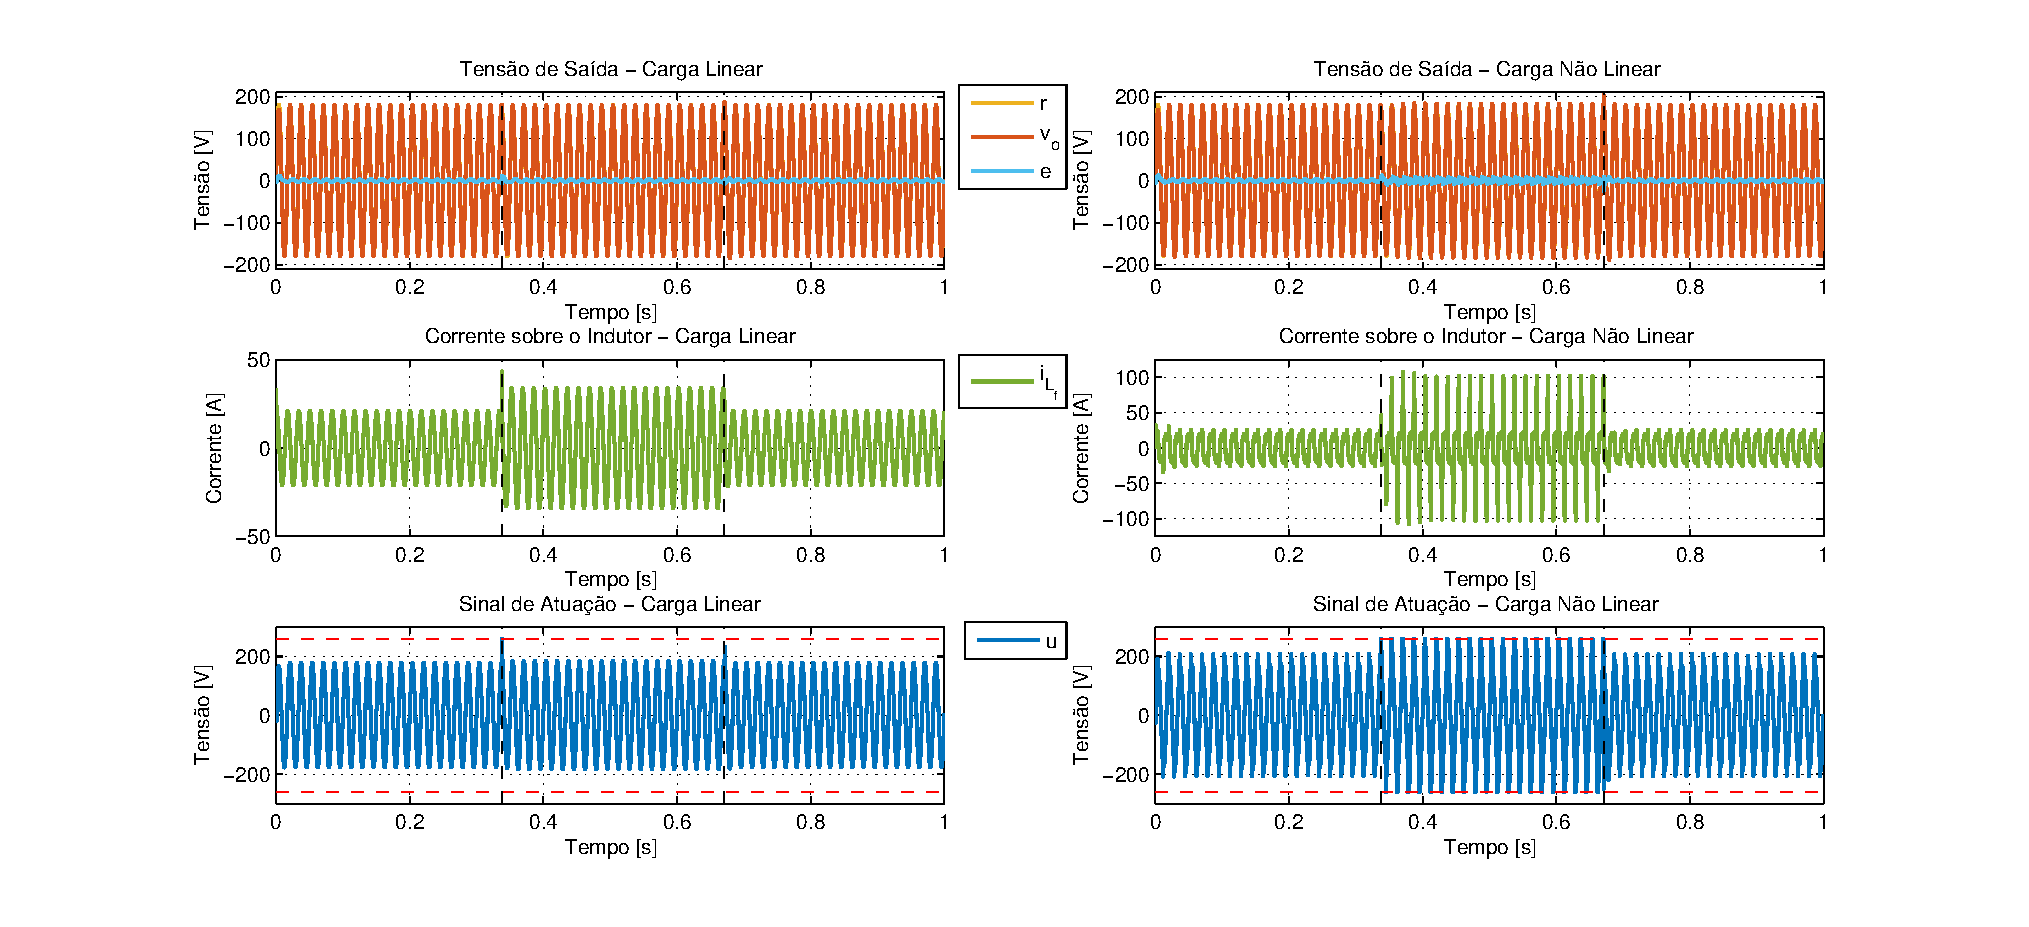
\includegraphics[trim={80 20 80 20}, clip, width=\linewidth]{fig/closed_7_full.eps}
    \\\sourcecitation{do autor}
    \label{fig:closed_7_full}
\end{figure}

%Para todos os casos, as distorções harmônicas com carga linear são muito menores que com a carga não linear.
Os resultados para a carga linear são, em todos os casos, melhores, em termos de fornecerem menores índices de distorção harmônica.
Assim, para poupar espaço, apresentam-se a seguir apenas os resultados obtidos na situação mais exigente, sob carga não linear.

A Figura \ref{fig:closed_7} apresenta o mesmo ensaio da Figura \ref{fig:closed_7_full}, agora porém detalhando os três eventos ocorridos sob carga não linear somente.
Observe que, nesta nova figura, os gráficos compartilham os mesmos eixos nos grupos verticais e horizontais, e os instantes dos degraus de carga são marcados com linhas tracejadas escuras.
A curva de tensão de saída permite verificar que o tempo de resposta projetado --- metade do primeiro ciclo da senoide --- é de fato atingido.
O mesmo ocorre nas respostas aos degraus de carga.
Nota-se, ainda, que sob carga máxima há momentos em que o sinal de atuação atinge brevemente os limites de saturação, sem que isso prejudique significativamente o desempenho.

\begin{figure}[!h]
    \centering
    \caption{Resposta em regime transiente com carga não linear utilizando o controlador para a frequência fundamental e a 3{\textordfeminine}, 5{\textordfeminine} e 7{\textordfeminine} harmônicas.}
    \includegraphics[trim={80 20 1 20}, clip, width=\linewidth]{fig/closed_7.eps}
    \\\sourcecitation{do autor}
    \label{fig:closed_7}
\end{figure}

\newpage
O desempenho quanto ao valor eficaz e componentes harmônicas é mostrado pela Figura \ref{fig:harm_7}, que retrata os mesmos instantes da Figura \ref{fig:closed_7}.
Novamente os gráficos compartilham os eixos nos grupos verticais e horizontais e os momentos dos degraus de carga são marcados com linhas tracejadas.
Verifica-se que, após cada evento, a tensão eficaz atinge rapidamente o valor nominal de $127 \text{ V\textsubscript{rms}}$.
As maiores distorções harmônicas, tanto em termos totais como individuais, ocorrem logo após os eventos, sendo brevemente atenuadas.
A exceção é a IHD de 9{\textordfeminine} ordem, que, sob 100\% da carga, cresce até um valor máximo.
Ora, visto que este controlador fora projetando considerando a frequência fundamental e a 3{\textordfeminine}, 5{\textordfeminine} e 7{\textordfeminine} harmônicas, este comportamento é esperado.
%Ainda assim, a 9{\textordfeminine} harmônica permanece dentro dos limites aceitáveis.

\begin{figure}[h]
    \centering
    \caption{Desempenho em regime transiente com carga não linear utilizando o controlador para a frequência fundamental e a 3{\textordfeminine}, 5{\textordfeminine} e 7{\textordfeminine} harmônicas.}
    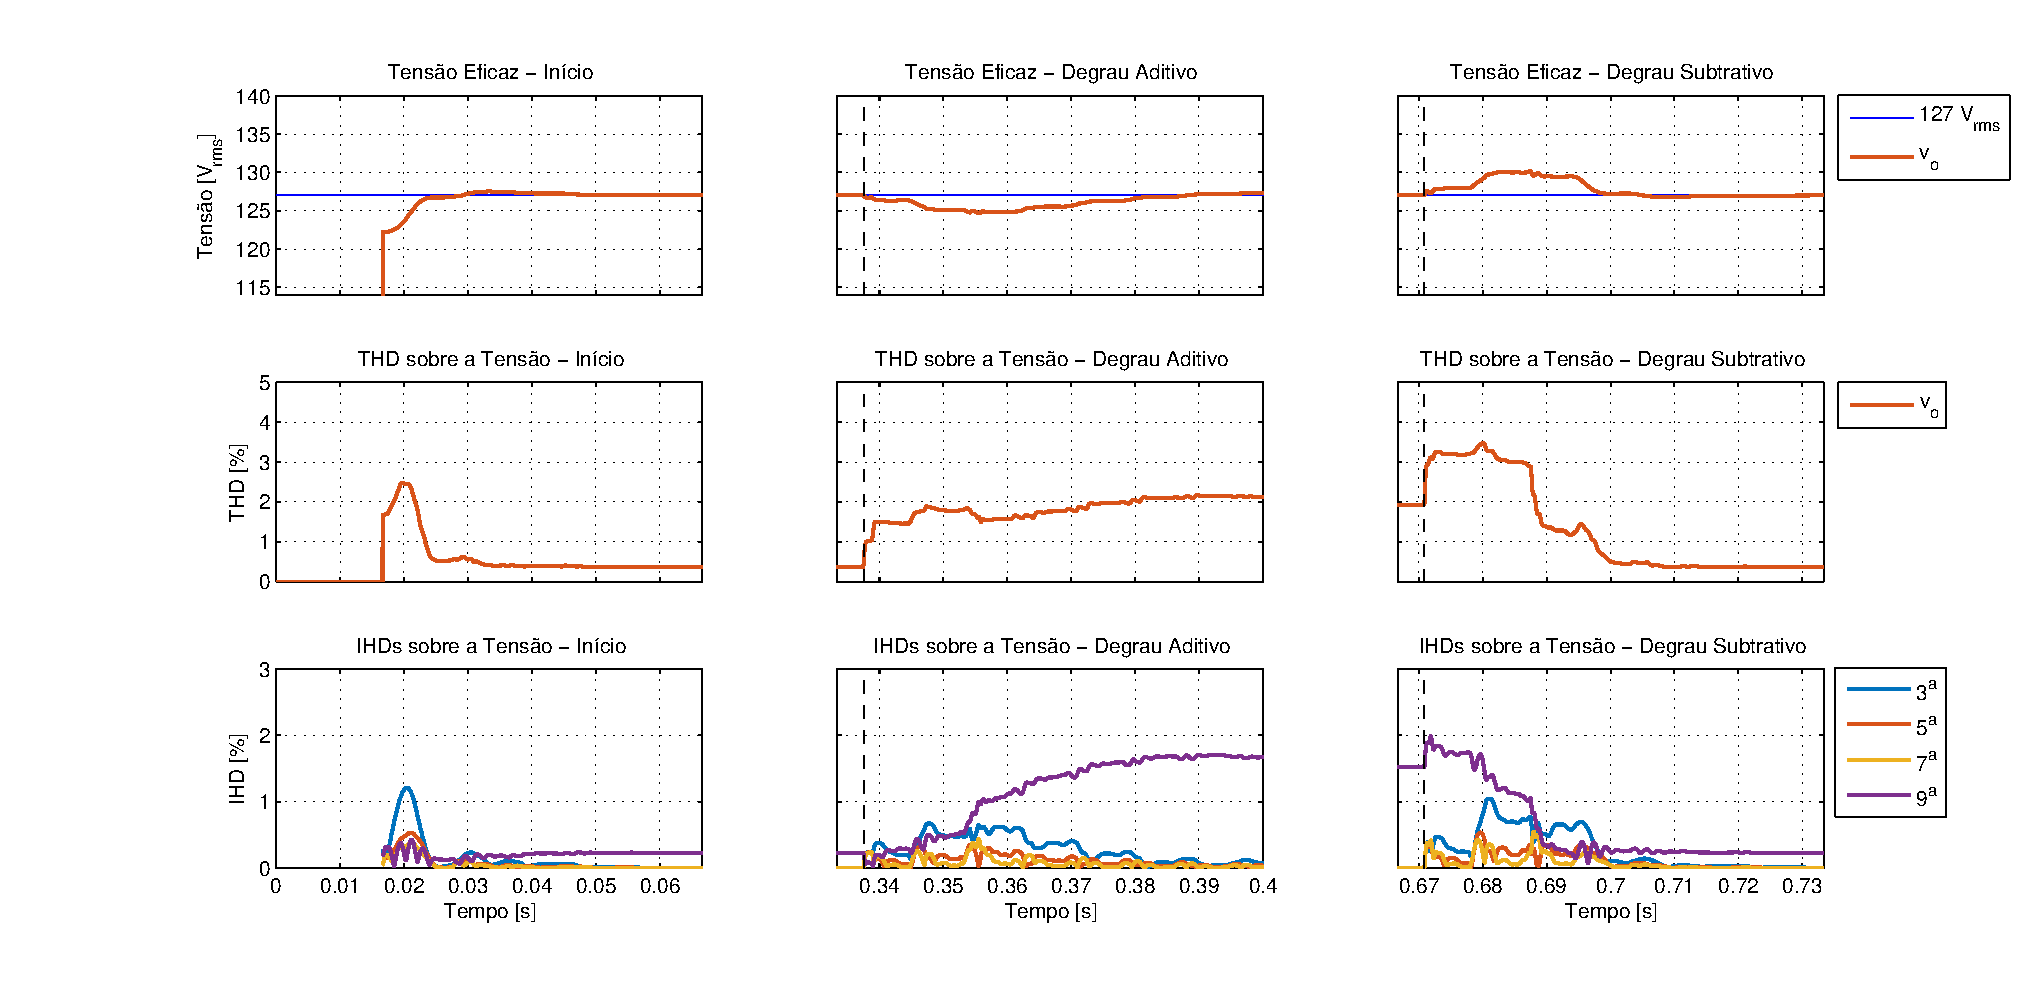
\includegraphics[trim={80 20 1 20}, clip, width=\linewidth]{fig/harm_7.eps}
    \\\sourcecitation{do autor}
    \label{fig:harm_7}
\end{figure}

\newpage
A avaliação do desempenho em regime transiente é realizada pela comparação com o perfil da Figura \ref{fig:IEC_DynamicVoltage1}.
O desvio relativo de tensão após aplicação dos degraus de carga não linear é exibido na Figura \ref{fig:iec_7}, em que os limites admissíveis estão reproduzidos.
A conformidade é atingida tanto para o degrau aditivo como para o subtrativo.

\begin{figure}[h]
    \centering
    \caption{Desvio relativo de tensão após degrau de carga não linear utilizando o controlador para a frequência fundamental e a 3{\textordfeminine}, 5{\textordfeminine} e 7{\textordfeminine} harmônicas.}
    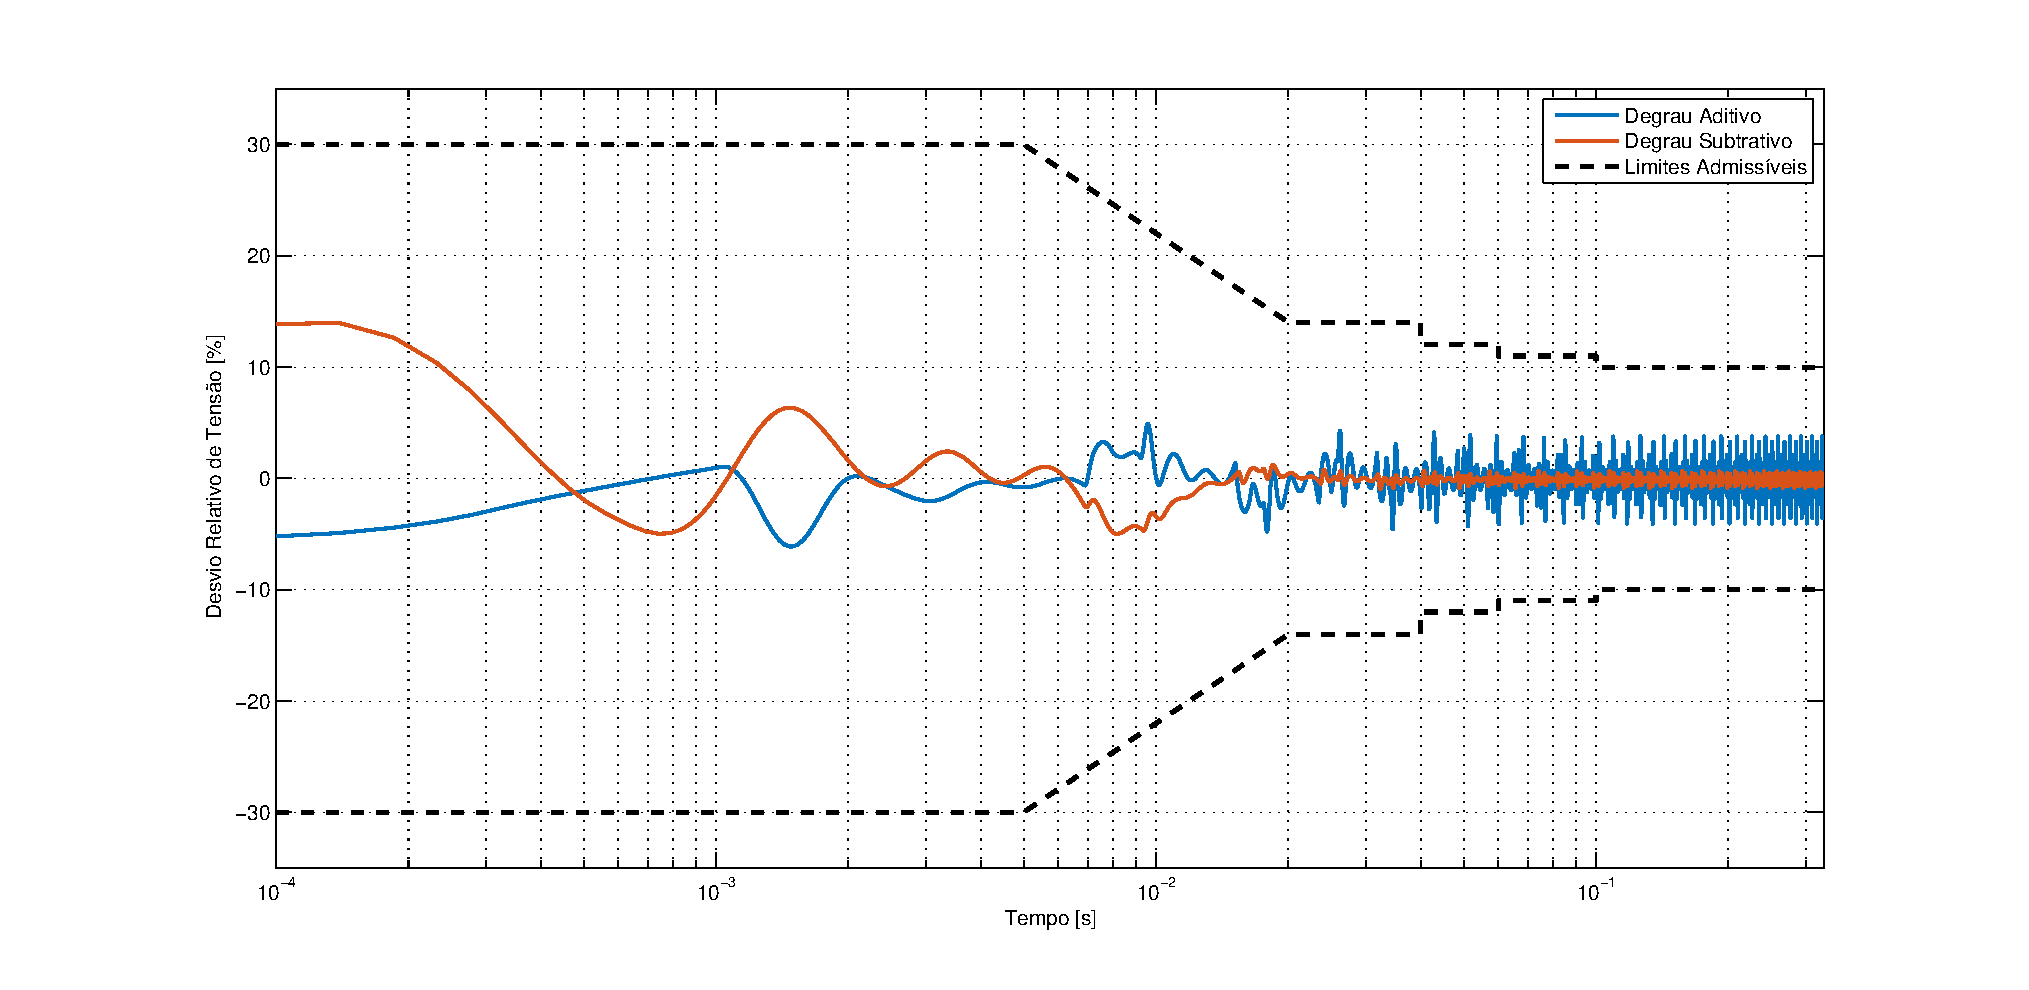
\includegraphics[trim={80 20 80 20}, clip, width=0.7\linewidth]{fig/IEC_7.eps}
    \\\sourcecitation{do autor}
    \label{fig:iec_7}
\end{figure}

Finalmente, a tensão eficaz e as distorções harmônicas em regime permanente são avaliadas em relação aos valores de referência.
Essa comparação é sintetizada através da Tabela \ref{tab:harm}, que inclui os resultados de todos os controladores projetados, exceto aquele que considera a 9{\textordfeminine} harmônica, para a carga não linear máxima, situação de maior exigência.

\begin{table}[h]
    \centering
    \caption{Avaliação do desempenho em regime permanente com 100\% da carga não linear.}
    %\resizebox{.9\textwidth}{!}{%
    \begin{tabular}{c|c|c|c|c|c}
                                                      & \multirow{2}{0.18\linewidth}{\centering\textbf{Valores Admissíveis}} & \multicolumn{4}{c}{\textbf{Ordem da Maior Harmônica}} \\
                                                      &                                                                      & \textbf{1} & \textbf{3} & \textbf{5} & \textbf{7}     \\\hline
        Tensão Eficaz [$\text{V\textsubscript{rms}}$] & $127 \pm 10\%$                                                       & $129,8$    & $127,5$    & $127,1$    & $127,0$        \\\hline
        THD [$\%$]                                    & $<8$                                                                 & $20,95$    & $8,75$     & $3,57$     & $1,93$         \\\hline
        IHD\textsubscript{3} [$\%$]                   & $<5$                                                                 & $20,43$    & $<0,001$   & $< 0,001$  & $< 0,001$      \\\hline
        IHD\textsubscript{5} [$\%$]                   & $<6$                                                                 & $4,24$5    & $7,94$     & $< 0,001$  & $< 0,001$      \\\hline
        IHD\textsubscript{7} [$\%$]                   & $<5$                                                                 & $1,57$     & $2,72$     & $2,93$     & $< 0,001$      \\\hline
        IHD\textsubscript{9} [$\%$]                   & $<1,5$                                                               & $0,98$     & $2,27$     & $1,13$     & $1,53$         \\
    \end{tabular}
    %}%
    \\\vspace{0.25cm}\sourcecitation{do autor}
    \label{tab:harm}
\end{table}

Em todos os casos, a tensão eficaz em regime permanente está dentro dos limites aceitáveis.
Observa-se que a inclusão de harmônicas como polos ressonantes no controlador efetivamente reduz a respectiva IHD para valores desprezíveis, menores que $0,001\%$.
Afirma-se, portanto, que cada um desses controladores cumpriu seu objetivo para as harmônicas consideradas no projeto.

No primeiro controlador, considerando apenas a frequência fundamental, verificam-se elevadas THD e IHD\textsubscript{3}, próximas a $20\%$ e comparáveis aos valores obtidos por \textcite{Corleta2016} sem o uso da realimentação de corrente.
A Tabela \ref{tab:rhos} revela que, de fato, o ganho de corrente $k_P$ obtido nesta sintonia é menor que nas demais.
Assim, nesse caso específico, o projeto por VRFT não forneceu resultados tão bons quanto esperados.

No controlador de ordem 3 verifica-se que a 3{\textordfeminine} harmônica é rejeitada com sucesso.
Essa rejeição, porém, veio ao custo de uma maior influência das demais harmônicas.
Ainda que a THD tenha sido reduzida, seu limite é novamente ultrapassado.
A IHD\textsubscript{5} também aparece acima do valor máximo.

Por sua vez, o controlador de ordem 5 apresenta atenuação da 3{\textordfeminine} e 5{\textordfeminine} harmônicas, sem tanta influência sobre as demais.
A THD é novamente reduzida e, dessa vez, todos os indicadores estão dentro dos limites de conformidade.

Finalmente, o controlador de ordem 7 proporciona rejeição da 3{\textordfeminine}, 5{\textordfeminine} e 7{\textordfeminine} harmônicas.
Embora a THD tenha sido reduzida ainda mais, a IHD\textsubscript{9} aparece levemente acima do máximo valor admissível.

Como visto, a rejeição de uma determinada harmônica tende a aumentar as distorções sobre as outras.
Este efeito, denominado colchão d'água, é explicado pela fórmula da integral de Bode, conforme demonstra \textcite{Bertoldi2019}.
Essencialmente, a atenuação de perturbações em uma determinada frequência ocasiona a amplificação dos distúrbios em outros locais do espectro frequencial.

O projeto considerando a 9{\textordfeminine} harmônica foi excluído da análise de desempenho em regime permanente porque não foi obtido nenhum controlador que mantenha o sistema estável sob o teste realizado.
Diversos controladores foram testados, obtidos a partir de diferentes posições de polos no modelo de referência.
Muitos deles são capazes de manter o seguimento da referência com carga linear e não linear, e alguns até mesmo após o degrau aditivo de carga.
Todos, porém, resultam em instabilidade após o degrau subtrativo de carga não linear, ou em outros momentos do ensaio.
%Sob carga máxima, esses controladores geram um sinal de controle saturante.
Em geral, a brusca variação da corrente no indutor no momento do degrau subtrativo faz com que o sinal de atuação alterne entre os limites da saturação e não se recupere.
Esse comportamento pode ser visualizado no Apêndice \ref{app:respostas}, Figura \ref{fig:closed_9_app}.
Cabe ainda destacar duas peculiaridades observadas na sintonia deste controlador, as quais podem ser vistas na Tabela \ref{tab:rhos}:
o número de iterações para convergência dos parâmetros é consideravelmente maior;
o parâmetro $k_{R_{5_1}}$ aparece com um valor negativo, sendo que em todos os outros casos os parâmetros $k_{R_{i_1}}$, para qualquer $i$, são sintonizados com valores positivos.

%\section{Comentários}

\chapter{Conclusões}\label{sec:conclusao}

Este trabalhou apresentou a aplicabilidade do método VRFT para sistemas em cascata através do projeto de dois controladores, sendo um PMR e outro P, a partir de um único conjunto de dados.
Ainda, comprovou-se que essa topologia e classes de controladores são capazes de atenuar significativamente as distorções harmônicas sob carga não linear.

Para tanto, propôs-se um modelo de referência capaz de prover o seguimento de referências oscilando na frequência fundamental e suas harmônicas ímpares.
Este modelo mostrou-se efetivo para controladores de menor ordem harmônica, mas não proporcionou uma boa sintonia quando a 9{\textordfeminine} harmônica passa a ser considerada.
Modelos alternativos, com diferentes posições de polos espalhadas pelo círculo unitário, potencialmente poderiam oferecer um melhor resultado.

Um inconveniente verificado é que, da maneira como foi formulado, o método VRFT permite definir um modelo de referência apenas para o sistema em malha fechada, isto é, da referência para a saída.
De fato, em sua concepção original, esta abordagem não considera a rejeição de perturbações.
Assim, para inibir as distorções harmônicas, este trabalho estabelece um modelo de referência capaz de também seguir senoides nessas frequências, obtendo a rejeição como um efeito secundário.
%Em \textcite{Lecchini2001}, os autores originais do VRFT propõem uma adaptação do método que permite a definição não só do modelo de referência para o sistema em malha fechada, mas também para a sensibilidade de perturbações na saída do processo.

Existe uma adaptação do VRFT, proposta pelos autores originais do método, \textcite{Lecchini2001}, que permite a definição não só do modelo de referência para o sistema em malha fechada, mas também para a sensibilidade de perturbações na saída do processo.
A topologia ali apresentada separa o controlador principal em dois:
o primeiro, manipulando diretamente o sinal de referência, é responsável apenas pelo seu seguimento;
o segundo, operando sobre o sinal de saída medido, atua tanto no seguimento da referência como também na rejeição de perturbações.
Sugere-se, assim, avaliar a viabilidade de adaptar esta topologia e a metodologia associada em conjunto com aquela apresentada por \textcite{Chrystian2020}, para a sintonia de três controladores simultâneos para a UPS:
o primeiro controlador apenas para o seguimento da tensão senoidal;
o segundo para seguimento da tensão e rejeição das harmônicas; e
o terceiro para melhora do desempenho dinâmico por realimentação de corrente no laço interno.

Outros dois efeitos indesejados foram verificados neste trabalho: a eventual saturação do sinal de atuação e o fenômeno do colchão d'água.
\textcite{Keiel2017, Keiel2019, Bertoldi2019} mostram que ambos os efeitos podem ser mitigados pela aplicação de amortecimento no controlador PMR.
Com isso, seu ganho nas frequências de interesse passa a ser finito.
Efetivamente, o controlador deixa de ser ressonante, podendo ser denominado \textit{quasi}-ressonante.
A utilização deste controlador resultaria numa rejeição parcial das distorções nas frequências selecionadas.
Ainda assim, com um coeficiente de amortecimento adequado, seria possível atender os limites de distorção estabelecidos pela norma \textcite{IEC62040-3:2011} sem comprometer tanto as outras frequências.
Além disso, o ganho finito está diretamente associado a redução do esforço de controle.

Devido às restrições sanitárias e, consequentemente, à suspensão de atividades presenciais na UFRGS no momento do desenvolvimento deste trabalho, não foi possível empregar a metodologia sobre a UPS real disponível no LASCAR.
A validação prática é deixada como outra sugestão de trabalho futuro.
Neste caso, a presença de ruído, principalmente na instrumentação, tende a afetar negativamente os resultados.
Para reduzir seu efeito no projeto, sugere-se a utilização de variáveis instrumentais através da coleta de dados de dois ensaios sob um mesmo sinal de excitação \cite{Campi2000}.

\appendix

\chapter{Projeto dos Controladores}\label{app:varia_polo}

Este apêndice contém os detalhes dos projetos de cada um dos controladores desenvolvidos, partindo pela consideração apenas da frequência fundamental até incorporar as harmônicas ímpares até a 9{\textordfeminine} ordem.
Para cada caso, e para diferentes valores de polos no modelo de referência, são exibidos o mapa de polos e zeros, diagrama de bode, e resposta a referência senoidal da função de transferência desejada, além do mapa de polos e zeros do respectivo controlador de tensão obtido.
%Para escolher o modelo de referência definitivo para os testes com a UPS, avalia-se a estabilidade dos zeros

\begin{figure}[!ht]
    \centering
    \caption{Efeito da variação dos polos do modelo de referência considerando apenas a frequência fundamental.}
    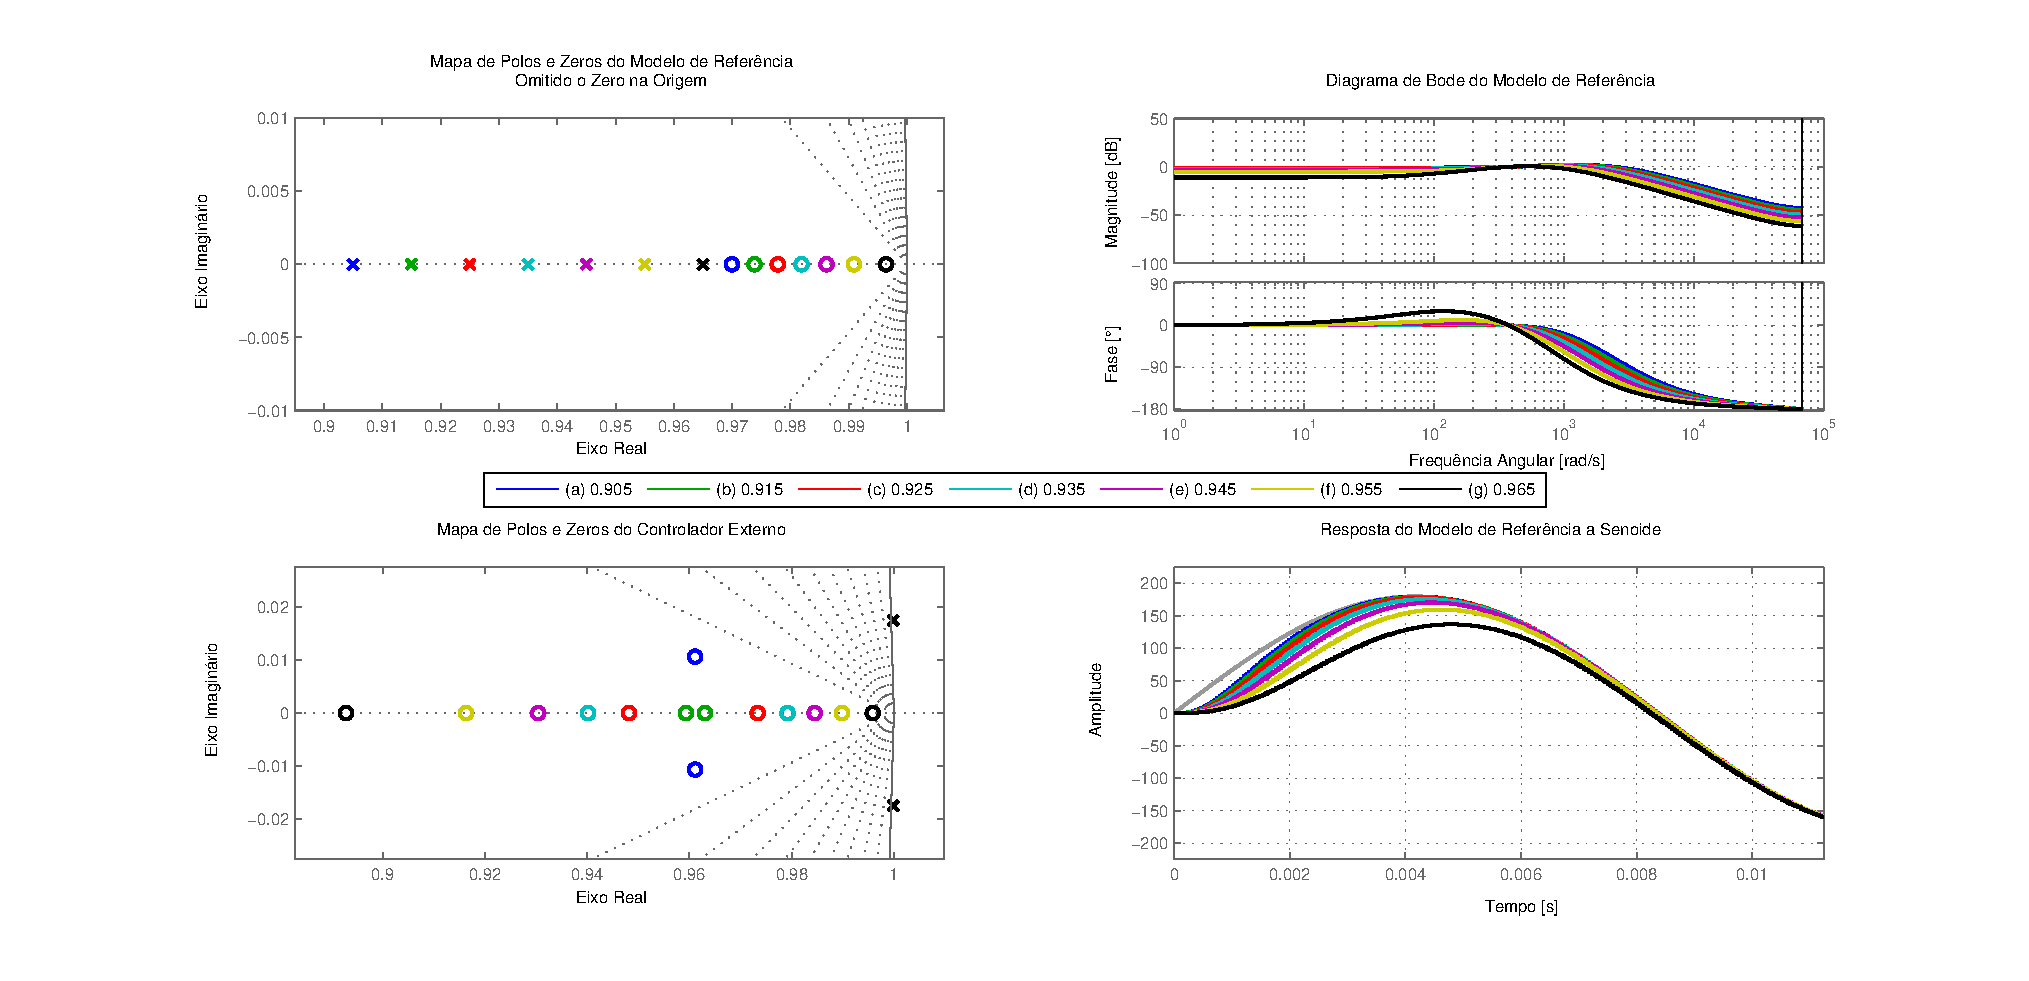
\includegraphics[trim={80 20 80 10}, clip, width=\linewidth]{fig/f_1.eps}
    \\\sourcecitation{do autor}
    % \label{fig:my_system1}
\end{figure}

\begin{figure}[!ht]
    \centering
    \caption{Efeito da variação dos polos do modelo de referência considerando a frequência fundamental e a 3{\textordfeminine} harmônica.}
    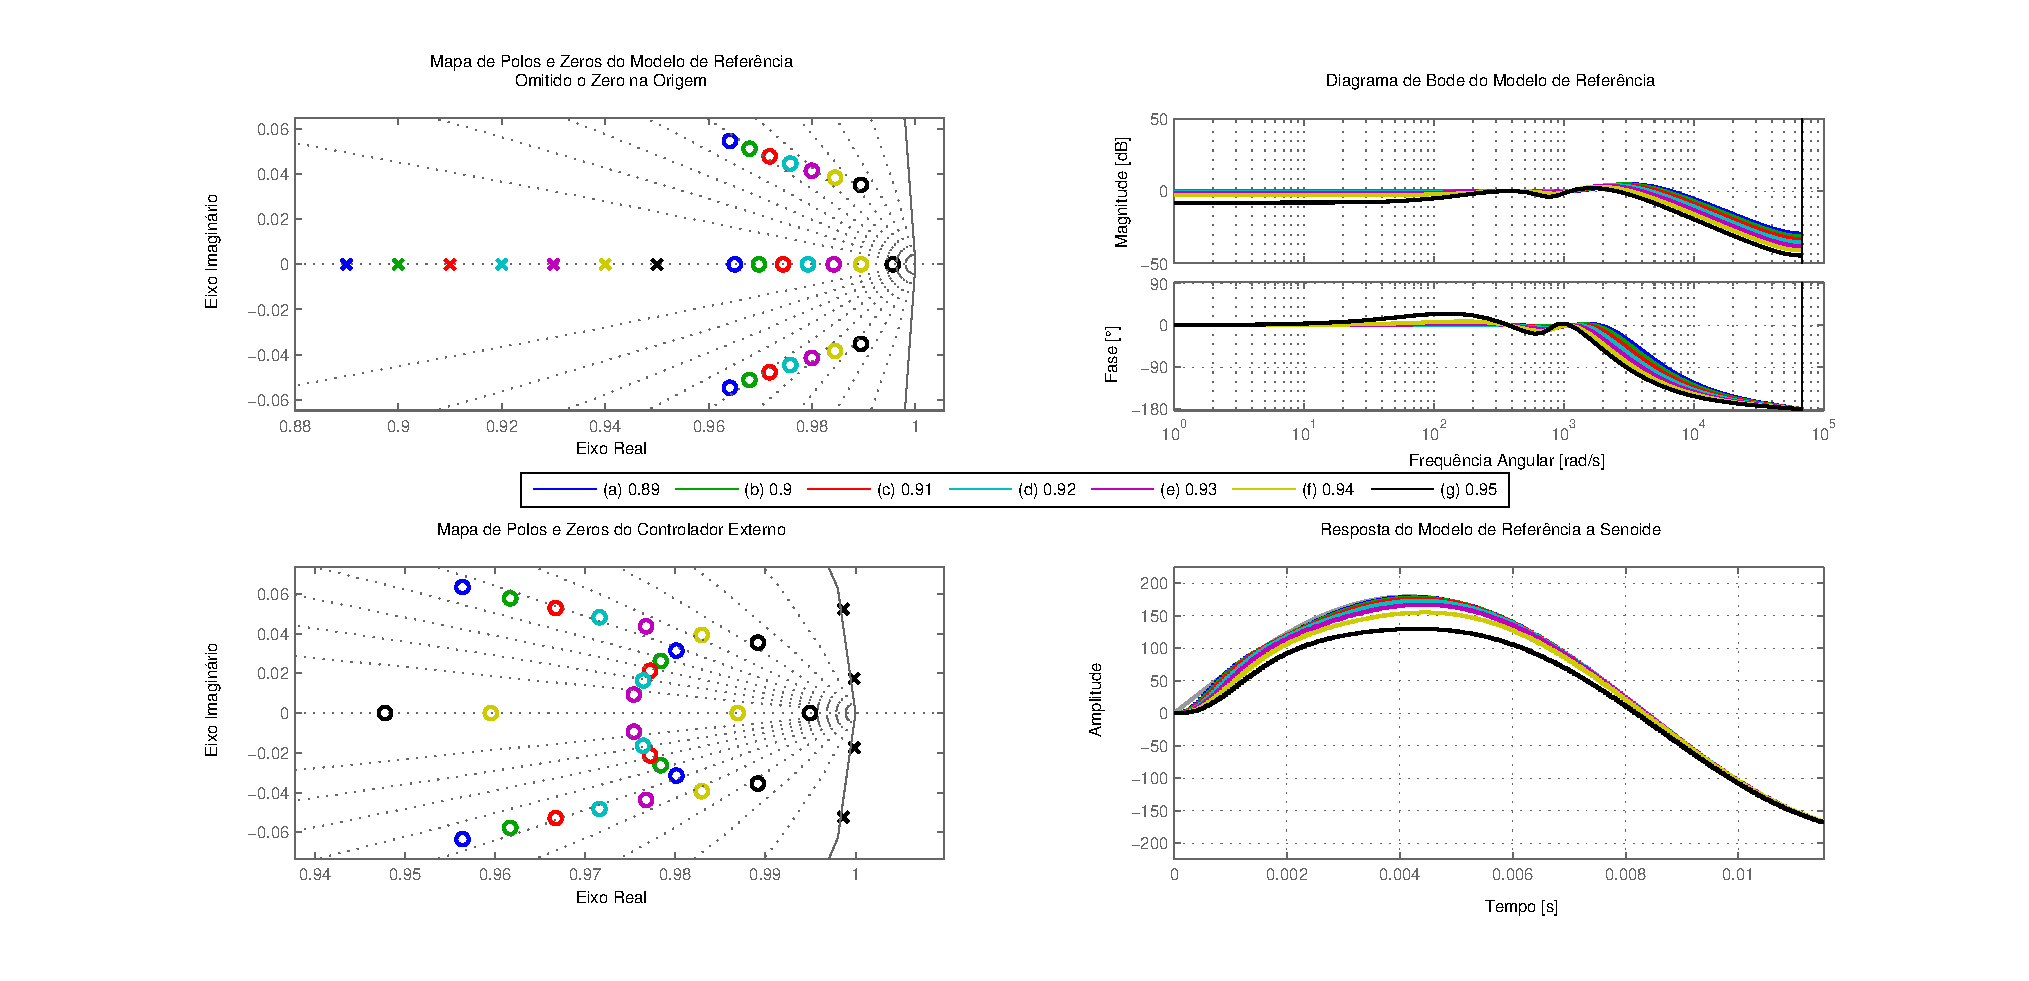
\includegraphics[trim={80 20 80 10}, clip, width=\linewidth]{fig/f_3.eps}
    \\\sourcecitation{do autor}
    % \label{fig:my_system3}
\end{figure}

\begin{figure}[!ht]
    \centering
    \caption{Efeito da variação dos polos do modelo de referência considerando a frequência fundamental e a 3{\textordfeminine} e 5{\textordfeminine} harmônicas.}
    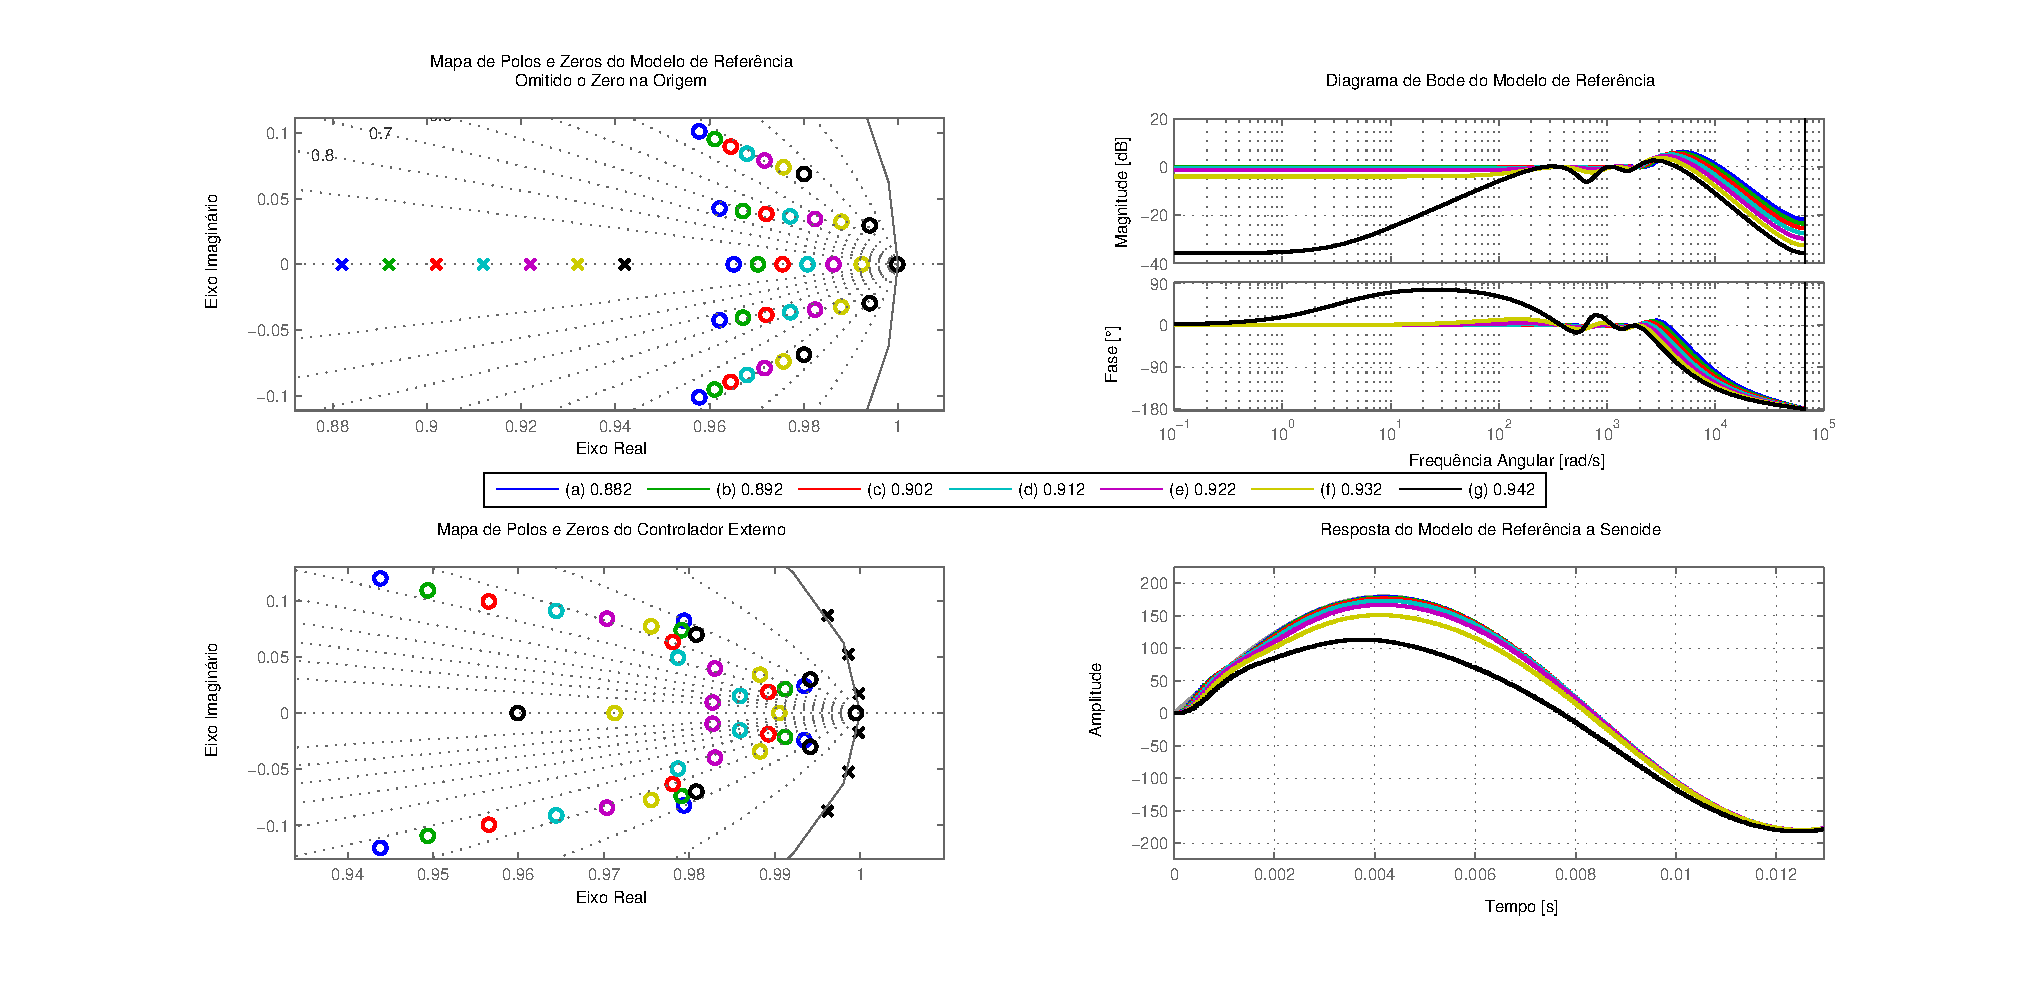
\includegraphics[trim={80 20 80 10}, clip, width=\linewidth]{fig/f_5.eps}
    \\\sourcecitation{do autor}
    % \label{fig:my_system5}
\end{figure}

\begin{figure}[!ht]
    \centering
    \caption{Efeito da variação dos polos do modelo de referência considerando a frequência fundamental e a 3{\textordfeminine}, 5{\textordfeminine} e 7{\textordfeminine} harmônicas.}
    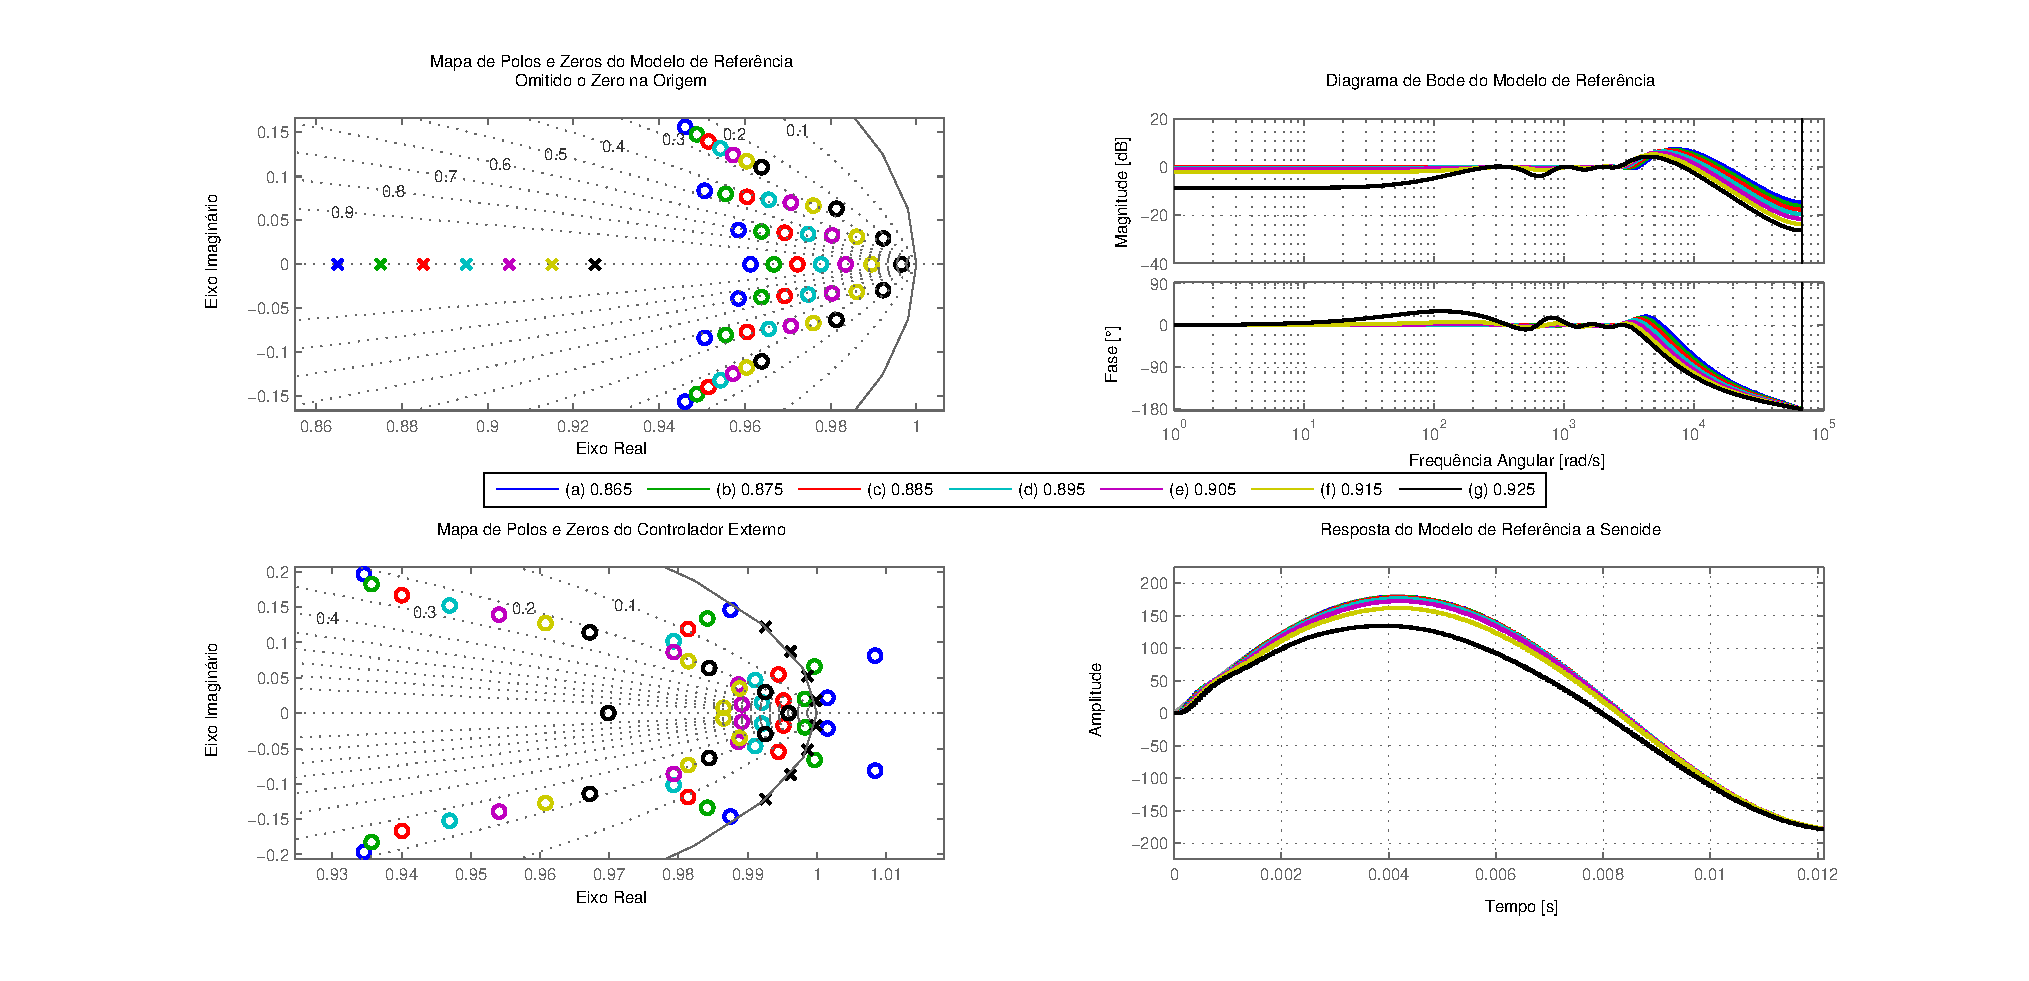
\includegraphics[trim={80 20 80 10}, clip, width=\linewidth]{fig/f_7.eps}
    \\\sourcecitation{do autor}
    % \label{fig:my_system7}
\end{figure}

\begin{figure}[!ht]
    \centering
    \caption{Efeito da variação dos polos do modelo de referência considerando a frequência fundamental e a 3{\textordfeminine}, 5{\textordfeminine}, 7{\textordfeminine} e 9{\textordfeminine} harmônicas.}
    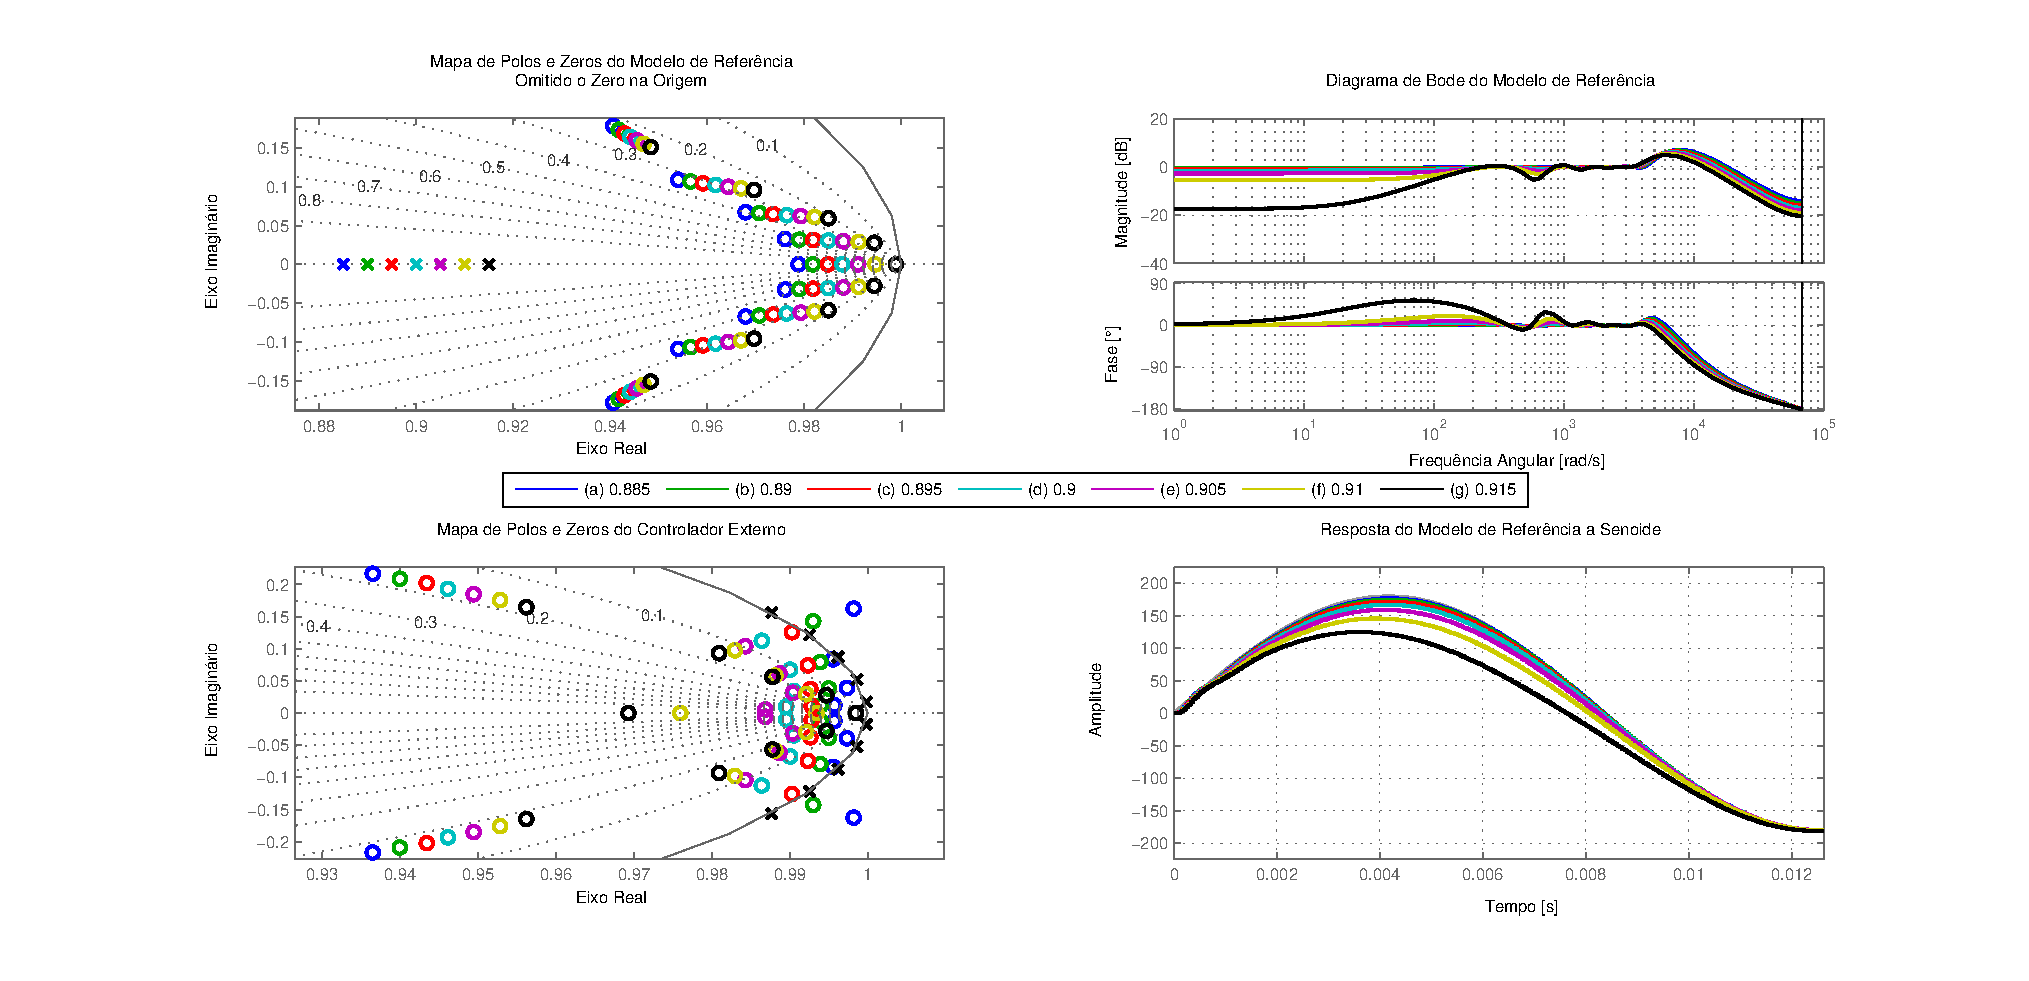
\includegraphics[trim={80 20 80 10}, clip, width=\linewidth]{fig/f_9.eps}
    \\\sourcecitation{do autor}
    % \label{fig:my_system9}
\end{figure}

\chapter{Respostas em Malha Fechada com Carga Não linear}\label{app:respostas}

Este apêndice reúne, para cada um dos controladores obtidos, os três eventos do ensaio em malha fechada sob carga não linear.
Em todos os casos, o controlador é aquele denotado pelo rótulo \texttt{(f)} no Apêndice \ref{app:varia_polo}.
Em cada figura, os gráficos compartilham os eixos nos agrupamentos verticais e horizontais.
Os instantes dos degraus de carga são identificados por linhas tracejadas escuras.

É importante destacar que, no último caso, considerando todas as harmônicas ímpares entre 3 e 9, o controlador não é capaz de manter o sistema estável após o degrau subtrativo de carga.
Ainda assim, julga-se interessante mostrar o resultado obtido.

\begin{figure}[h]
    \centering
    \caption{Resposta e desempenho em regime transiente com carga não linear utilizando o controlador para a frequência fundamental.}
    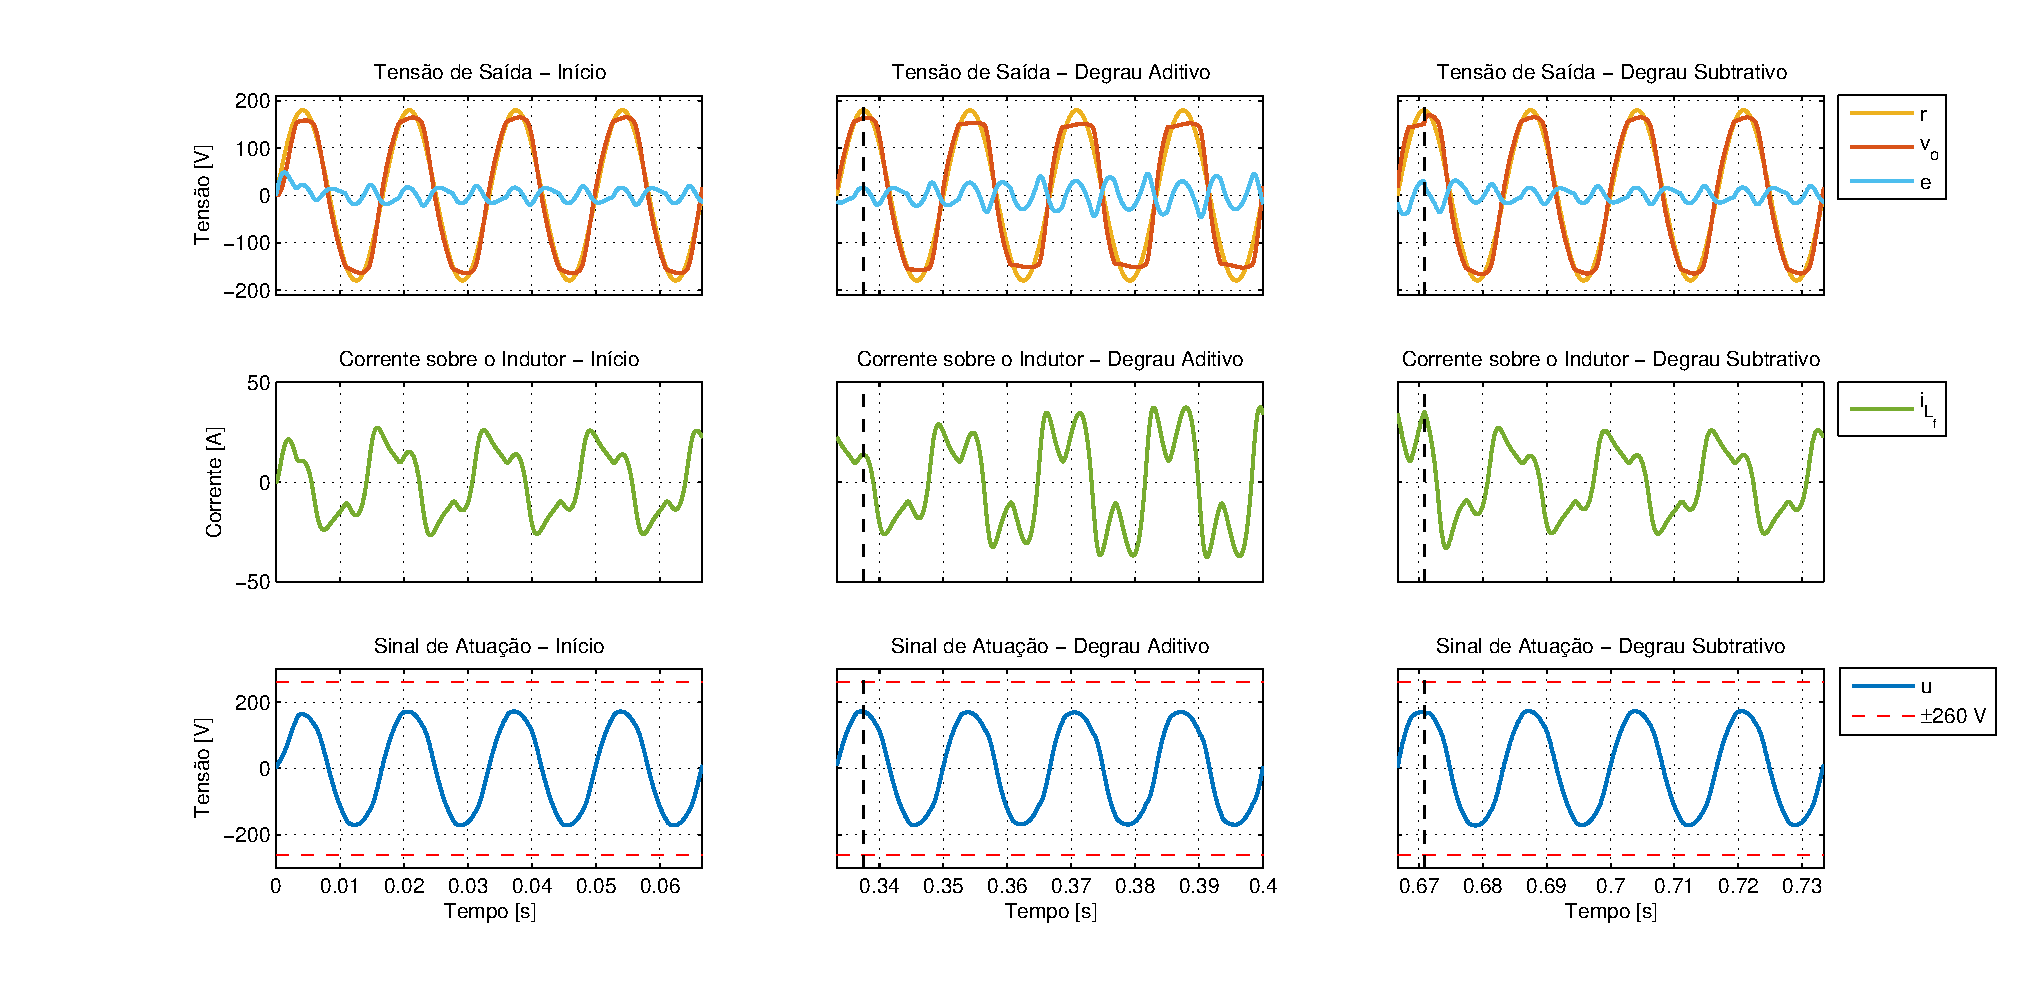
\includegraphics[trim={80 50 1 20}, clip, width=\linewidth]{fig/closed_1.eps}
    \\\vspace{0.475cm}
    \includegraphics[trim={80 20 1 20}, clip, width=\linewidth]{fig/harm_1.eps}
    \sourcecitation{do autor}
    % \label{fig:closed_1}
\end{figure}


\begin{figure}[h]
    \centering
    \caption{Resposta e desempenho em regime transiente com carga não linear utilizando o controlador para a frequência fundamental e a 3{\textordfeminine} harmônica.}
    \includegraphics[trim={80 50 1 20}, clip, width=\linewidth]{fig/closed_3.eps}
    \\\vspace{0.475cm}
    \includegraphics[trim={80 20 1 20}, clip, width=\linewidth]{fig/harm_3.eps}
    \sourcecitation{do autor}
    % \label{fig:closed_3}
\end{figure}

\begin{figure}[h]
    \centering
    \caption{Resposta e desempenho em regime transiente com carga não linear utilizando o controlador para a frequência fundamental e a 3{\textordfeminine} e 5{\textordfeminine} harmônicas.}
    \includegraphics[trim={80 50 1 20}, clip, width=\linewidth]{fig/closed_5.eps}
    \\\vspace{0.475cm}
    \includegraphics[trim={80 20 1 20}, clip, width=\linewidth]{fig/harm_5.eps}
    \sourcecitation{do autor}
    % \label{fig:closed_5}
\end{figure}

\begin{figure}[h]
    \centering
    \caption{Resposta e desempenho em regime transiente com carga não linear utilizando o controlador para a frequência fundamental e a 3{\textordfeminine} e 5{\textordfeminine} e 7{\textordfeminine} harmônicas.}
    \includegraphics[trim={80 50 1 20}, clip, width=\linewidth]{fig/closed_7.eps}
    \\\vspace{0.475cm}
    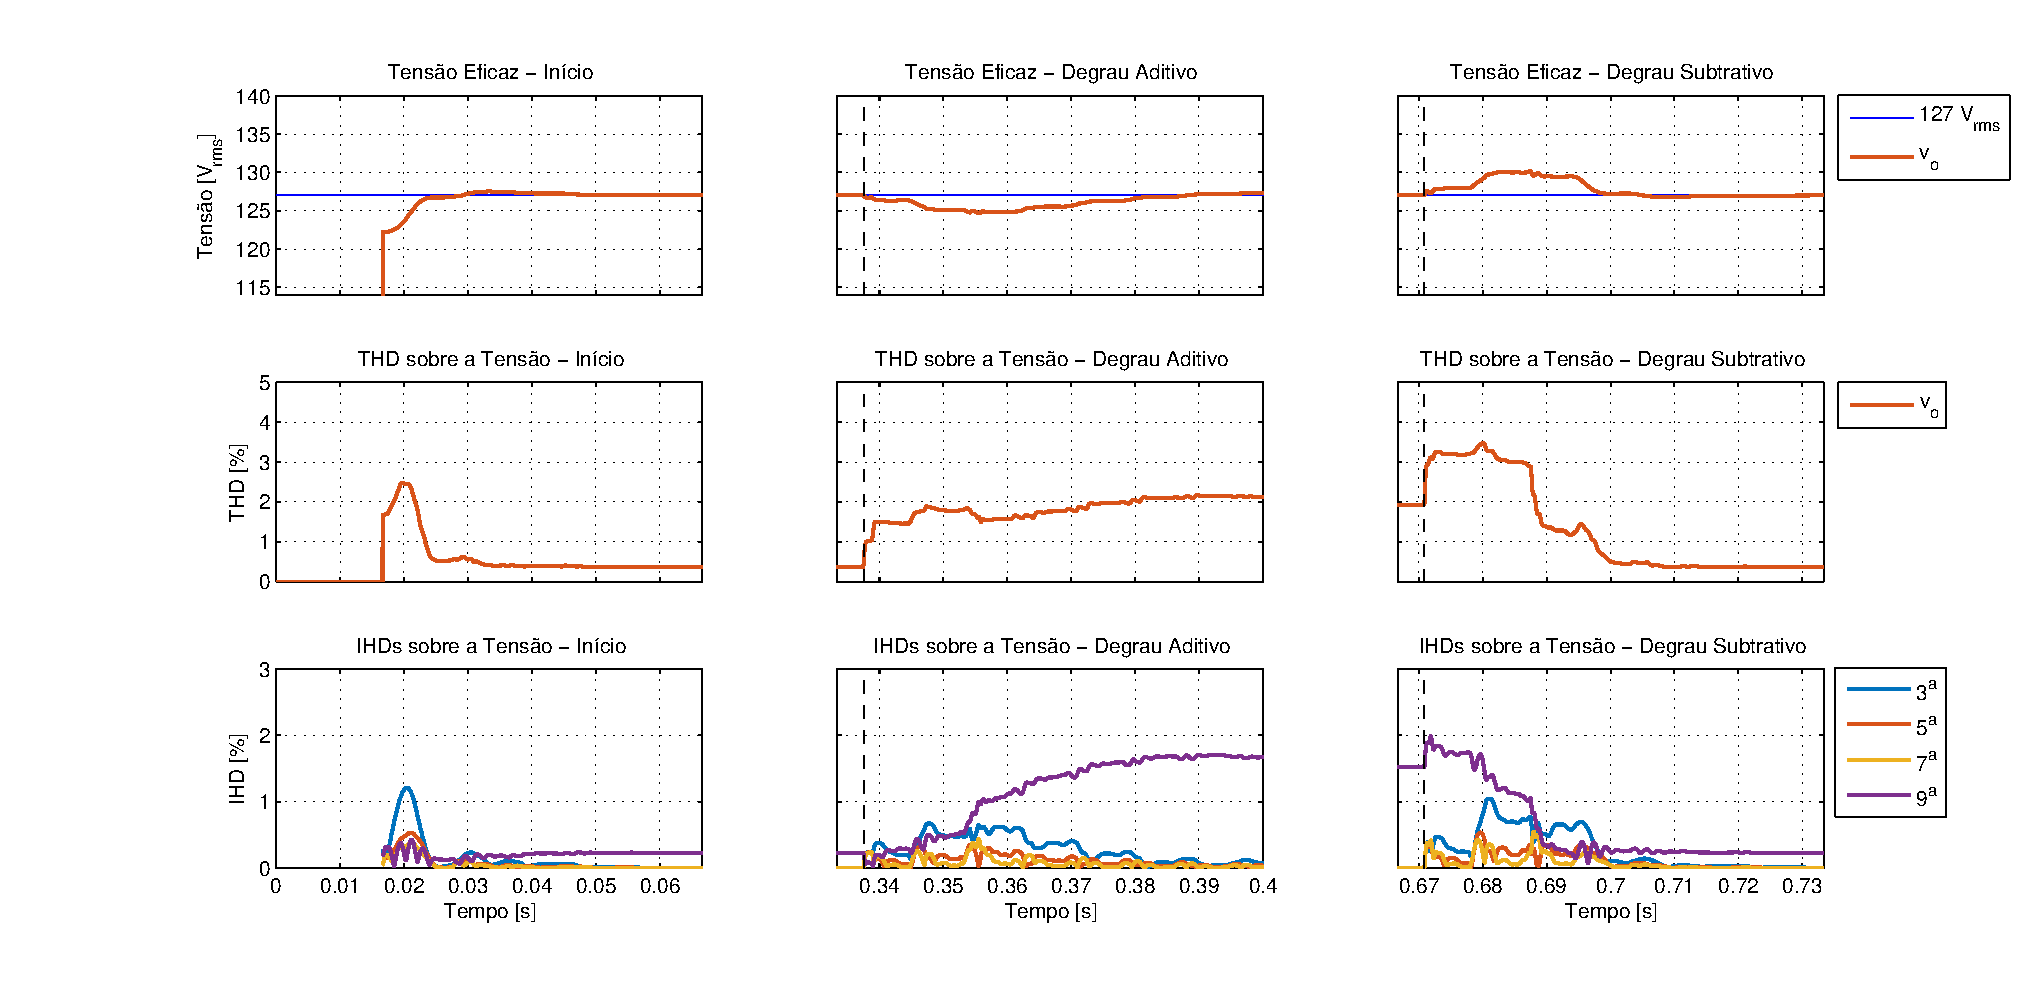
\includegraphics[trim={80 20 1 20}, clip, width=\linewidth]{fig/harm_7.eps}
    \sourcecitation{do autor}
    % \label{fig:closed_7_app}
\end{figure}

\begin{figure}[h]
    \centering
    \caption{Resposta e desempenho em regime transiente com carga não linear utilizando o controlador para a frequência fundamental e a 3{\textordfeminine} e 5{\textordfeminine}, 7{\textordfeminine} e 9{\textordfeminine} harmônicas.}
    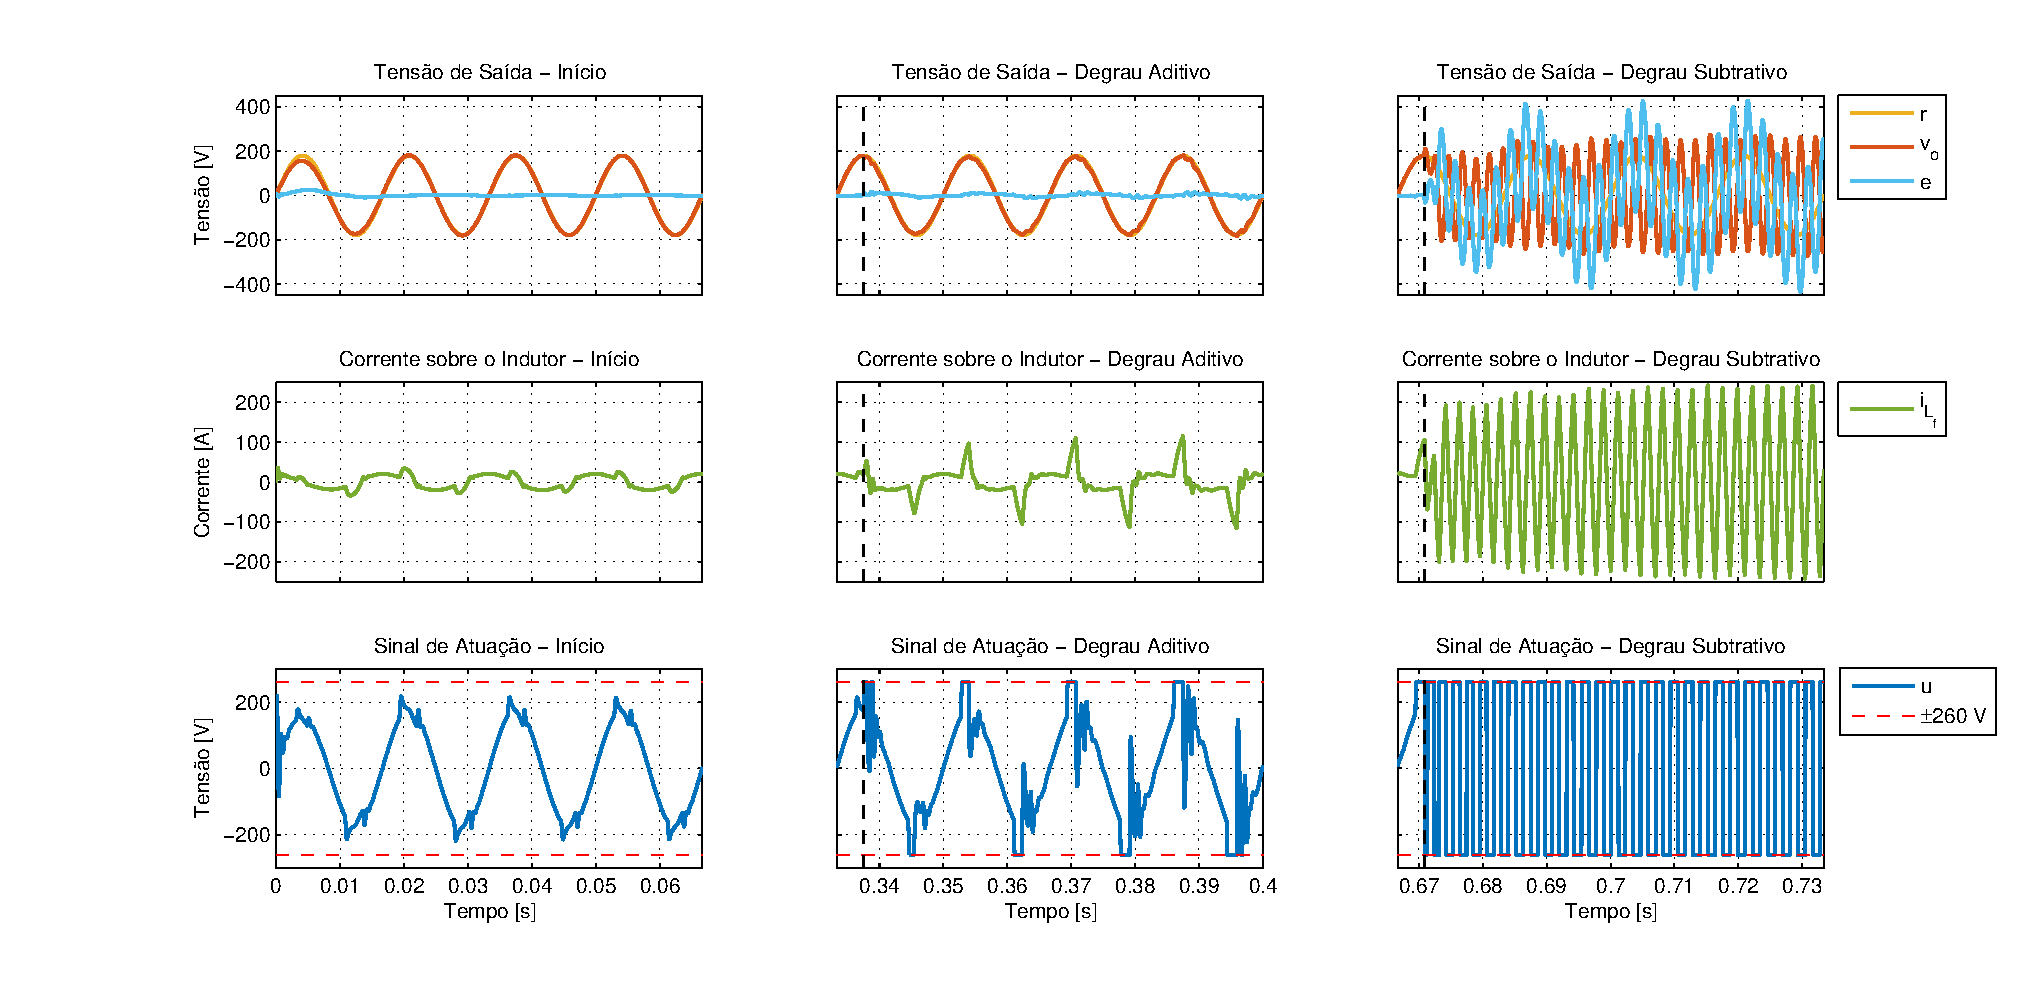
\includegraphics[trim={80 50 1 20}, clip, width=\linewidth]{fig/closed_9.eps}
    \\\vspace{0.475cm}
    \includegraphics[trim={80 20 1 20}, clip, width=\linewidth]{fig/harm_9.eps}
    \sourcecitation{do autor}
    \label{fig:closed_9_app}
\end{figure}

\annex

\printbibliography

\end{document}

